%!TEX root = istgame-doc.tex
%\begin{document}

\setcounter{section}{-1}

\section{Changes and remarks}

\subsection{Changes in version 2.1}
\label{ssec:changes2.1}

Version 2.1 of the \pkg{istgame} package introduces a starred version of the \env{istgame} environment, some new macros, and some examples added to the documentation.

\paragraph {The starred version of \env{istgame} environment:} The \emph{new} starred version of the \env{istgame} environment is essentially the same as the \env{tikzpicture} environment.
\begin{itemize}
\item The standard version of \env{istgame} environment checks the existence of \Tikz\ scaling and the arrow option |->|, and uses the collected information to automatically get the best results. (See Section~\ref{ssec:envistgame} on page~\pageref{ssec:envistgame} for more details.)
\item |\begin{istgame}*| may be slightly faster than |\begin{istgame}| as it does not collect this information.
\item However, using |\begin{istgame}*| may require some manual work to get desired results, especially for asymmetric \Tikz\ scaling (i.e. when |xscale| is not the same as |yscale|).
\item With |\begin{istgame}*|:
  \begin{itemize}
  \item |\xtxscale|, |\xtyscale|, and |\xtscale| have no effect.
  \item |\xtcureslopedlabelsNS| and |\xtcureslopedlabelsEW| do nothing.
  \item The oval type information sets |\xtInfosetO|, |\xtCIfnosetO|, and |\cntmAInfosetO| may be distorted.
  \item |\setistgamefontsize| and |\setistgameshorten| have no effect.
  \item The initial \Tikz\ arrow style (but not |>=stealth|) is used.
  \end{itemize}
%\end{istgame}
%\end{tikzpicture}
%\end{istgame}
%\end{istgame}
%\end{istgame}
\end{itemize}

It is recommended to use the standard \env{istgame} environment, 
when you use the oval type information sets and sloped labels with \Tikz\ scaling.
\emph{In all other cases}, |\begin{istgame}*| and |\begin{istgame}| will give you the \emph{same results} in drawing tree structures (except for the default arrow style).

\xbigskip1
Here are some examples to show that the \env{istgame} environment can automatically achieve the best results.

\begin{doccode}{.3}
% asymmetric scaling: distorted oval information sets
\begin{istgame}*[xscale=1.5,yscale=.9] % starred
\setistgrowdirection'{south east}
\istroot(0)          \istb  \istb* \endist
\istroot(1)(0-1){2}  \istb* \istb* \endist
\xtInfosetO[fill=red!20,ellipse](0)(0-2){1}
\xtInfosetO(1)(1)
\xtInfosetO[fill=blue!40,opacity=.5]
           (1-1)(1-2){3}(1.5em)
\end{istgame}
\end{doccode}

\begin{doccode}{.3}
% Oval information sets do not depend on scaling
\begin{istgame}[xscale=1.5,yscale=.9]
\setistgrowdirection'{south east}
\istroot(0)          \istb  \istb* \endist
\istroot(1)(0-1){2}  \istb* \istb* \endist
\xtInfosetO[fill=red!20,ellipse](0)(0-2){1}
\xtInfosetO(1)(1)
\xtInfosetO[fill=blue!40,opacity=.5]
           (1-1)(1-2){3}(1.5em)
\end{istgame}
\end{doccode}


The \Tikz's |tree| library does not seem to deal with the sloped labels correctly in the case of asymmetric scaling. (See page~\pageref{page:slopedlabels-warning} for more details.)

\begin{doccode}{.3}
% tikz tree's sloped labels problem:
\begin{istgame}*[xscale=2,font=\footnotesize] % starred
\xtcureslopedlabelsNS % does nothing
\istroot(0)
  \istb[dashed,thick]{Left}[above,sloped]
  \istb[->]{Center}[above,sloped]
  \istb[draw=blue,thick]{Right}[above,sloped]
  \endist
\end{istgame}
\end{doccode}

The macro |\xtcureslopedlabelsNS| solves this problem only when you use the standard version of \env{istgame}.

\begin{doccode}{.3}
% tikz tree's sloped labels problem: solved
\begin{istgame}[xscale=2,font=\footnotesize]
\xtcureslopedlabelsNS
\istroot(0)
  \istb[dashed,thick]{Left}[above,sloped]
  \istb[->]{Center}[above,sloped]
  \istb[draw=blue,thick]{Right}[above,sloped]
  \endist
\end{istgame}
\end{doccode}

\paragraph{New macros to set the default node sizes:}
In order to change the size of basic nodes, new macros \icmd{\setistsolidnodesize}, \icmd{\setisthollownodesize}, \icmd{\setistellipsenodesize}, and \icmd{\setistrectanglenodesize} are introduced. You can use these macros outside of the \env{istgame} environment (or in the preamble) to change the default node size globally.

In the following example you can see the effect of |\setistsolidnodesize{.5\pgflinewidth}|. The default size of a |solid| node is |2.4pt|.

\begin{doccode}[text above listing]
% \setistsolidnodesize
\begin{istgame}
\istroot(0)(0,0) \istb* \istb* \istb* \endist
\istroot(c)(0-3) \istb* \istb* \endist
\setistsolidnodesize{.5\pgflinewidth} % solid node size changed
\istroot(0)(6,0) \istb* \istb* \istb* \endist
\istroot(c)(0-3) \istb* \istb* \endist
\end{istgame}
\end{doccode}


\paragraph{Some more:}
The update to version 2.1 includes a few bug fixes and minor changes.
(See the version history on page~\pageref{version-history}.)

The \Tikz\ libraries |arrows.meta| and |bending| are added to the the list of preloaded |tikz| libraries. You can see some examples of arrow tips from |arrows.meta| in Section~\ref{ssec:setxtarrowtips} on page~\pageref{ssec:setxtarrowtips}.

\subsection{Changes in version 2.0}

Some macros have been \textsc{changed} and \textsc{removed} in version 2.0.
Those who have used these changed and removed macros may want to \textsc{find} and \textsc{replace} the followings:

%\begin{center}
%\begin{tabu}  {X[l1.5]X[l1.5]}  \toprule %to .5\linewidth
%\makecell[l]{\textbf{ver. 1.0}} & \makecell[l]{\textbf{ver. 2.0 or later}} \\\midrule
%|\istb.| & |\istbt| \\\tabucline- 
%|\xtInfoset'| & |\xtInfoset| \\\tabucline- 
%|\xtInfosetO'| & |\xtInfosetO| \\\tabucline- 
%|\setistgrowkey| & |\setxtgrowkey| \\\tabucline- 
%\end{tabu} 
%\end{center}

\begin{center}
\begin{tabular}  {lll}  \toprule 
\makecell[l]{\textbf{ver. 1.0}} & \makecell[l]{\textbf{ver. 2.0 or later}} \\\midrule
|\istb.| & |\istbt| \\\cline{1-2} 
|\xtInfoset'| & |\xtInfoset| \\\cline{1-2} 
|\xtInfosetO'| & |\xtInfosetO| \\\cline{1-2} 
|\setistgrowkey| & |\setxtgrowkey| \\\cline{1-2} 
\end{tabular} 
\end{center}

\paragraph{Changed and removed macros}

\begin{itemize}\tightlist
  \item The macro name |\istb.|(terminal version) has been changed 
        to |\istbt| (terminal version).   
  \begin{itemize}
  \item This is the opportunity cost of having a new macro |\istB| (dual action label version).
  \end{itemize}
\item The two (unsatisfactory) macros |\xtInfoset'| and |\xtInfosetO'| have been removed.
  \begin{itemize}
  \item The macro |\xtInfosetO| is completely redesigned, 
        so that we do not need the macro |\xtInfosetO'| any more.
  \item No reasons could be found to keep (even for the backward compatibility) 
        the swap versions |\xtInfoset'| and |\xtInfosetO'|, 
        except for the inconvenience to do `find and replace.'
  \end{itemize}
\item|\setistgrowkey| is renamed to |\setxtgrowkey| for consistency in macro naming.
\end{itemize}


\paragraph{Redesigned macros and the environment}

\begin{itemize}\firmlist
\item |\xtInfosetO| is completely redefined to improve its function:
  \begin{itemize}
  \item Now a \emph{sloped} information set is possible.
  \item It connects two nodes like |\xtInfosetO(coor1)(coor2)|, 
        but if the two coordinates are identical it represents a \emph{singleton information set} 
        by a \emph{circle} by default.
  \item This change does not seem to cause much harm, but be aware that 
        the swap version |\xtInfosetO'| has been removed and replaced by |\xtInfosetO|.
  \item Be aware also that the way to change the \emph{height} (|1em| by new default) 
        of an information set has been \emph{changed}, 
        though you might not see much difference if you have only used the default information sets.
  \item With \emph{new macros} |\xtCInfoset| and |\xtCInfosetO|, a curved (even skewed curved) information set is now possible.
  \end{itemize}
\item \env{istgame} environment: (internal change)
  \begin{itemize}
  \item Now the each value of the option of |xscale| and |yscale|, if exists, 
        is extracted and saved at |\xtxscale| and |\xtyscale|, respectively.
        The value of |scale| is also saved at |\xtscale| 
        only when it is used without |xscale| nor |yscale|. 
        These values are internally used to get the best outputs of trees in many ways.
  \item If the \Tikz\ arrow option |->| exists in the option list of an \env{istgame} environment, 
        you can globally control the arrow-end-shorten value (by default, |shorten >=0pt|) 
        by using a new macro |\setistgameshorten|. 
        This is to get a better result of branches with arrows.
  \end{itemize}
\item Some changes that you might not notice have been made, including:
  \begin{itemize}
  \item The core macros |\istroot|, |\istb|, and |\endist| have literally been redefined 
        for some purposes, but this makes no difference to users.
  \item The options |thin| and |solid| have been added to the definitions of basic node styles.
  \item Some default values have been slightly changed.
  \end{itemize}
\end{itemize}


\subsection{What's new in version 2.0}

\paragraph{Some new functions}

\begin{itemize}\tightlist
\item \emph{input mode changer} (math or text) for important labels: owners, action labels, and payoffs
  \begin{itemize}\tightlist
  \item |\setistmathTF| as an input mode changer for the important labels
  \item |\setistmathTF*| having additional functions as a \emph{text font style changer}
  \end{itemize}
\item \emph{curved} (even \emph{skewed}) \emph{information sets}
  \begin{itemize}\tightlist
  \item |\xtCInfoset| for curved information sets
  \item |\xtCInfosetO| for curved bubble type information sets
  \end{itemize}
\item enhanced \emph{continuum of branches} (making |\istcntm| and |\istcntmarc| obsolete)
  \begin{itemize}\tightlist
  \item |\istrootcntm| for a continuum triangle
  \item |\istrootcntmA| for a continuum arc (with |\istbA|)
  \item |\cntmAInfoset| and |\cntmAInfosetO| for information sets for a continuum of branches
  \end{itemize}
\item \emph{arrows} and \emph{middle arrows} on branches
  \begin{itemize}\tightlist
  \item controllable arrow option |->-| with |\setxtarrowtips| and middle arrow tip styles
  \item |\xtShowMidArrows| and |\xtShowArrows|
  \end{itemize}
\item and some more
  \begin{itemize}
  \item |\istB| for dual action labels
  \item |\xtTimeLineH|, |\xtTimeLineV|, |\xtCommentTo|, |\xtCommentFrom|, etc.
  \end{itemize}
\end{itemize}

\paragraph{List of new macros}
\begin{itemize}\tightlist
\item |\istbt(*)|: terminal version of |\istb(*)| 
      (replacement of the removed macro |\istb.(*)|)
\item |\istB(*)|: dual action label version of |\istb(*)|
\item |\istBt(*)|: terminal version of |\istB(*)|
\item |\istbA(*)|: alternative version of |\istb(*)| (intended to work with a continuum arc)
\item |\istbAt(*)|: terminal version of |\istbA(*)|
%
\listdivider

\item |\setistmathTF|: input mode changer (math or text) for owners, action labels, and payoffs
%  \begin{itemize}\tightlist
%  \item |\istownermathtrue|, |\istactionlabelmathtrue|, |\istpayoffmathtrue|: math mode
%  \item |\istownermathfalse|, |\istactionlabelmathfalse|, |\istpayoffmathfalse|: text mode
%  \end{itemize}
\item |\setistmathTF*|: input mode and font style changer for owners, action labels, and payoffs
%  \begin{itemize}\tightlist
%  \item |\istownertextfont|, |\istactionlabeltextfont|, |\istpayofftextfont|
%  \end{itemize}
%
\listdivider

\item |\xtCInfoset|: (curved version) curved information set
\item |\xtCInfosetO|: (curved oval version) curved oval type information set
\item |\xtCInfosetOTurnX|: turns |X| circles of |\xtCInfosetO| (to use it just in case)
%
\listdivider

\item |\xtInfoset*|: prints owners according to the input mode as set by |\setistmathTF(*)|
\item |\xtInfosetO*|: prints owners according to the input mode as set by |\setistmathTF(*)|
\item |\xtCInfoset*|: prints owners according to the input mode as set by |\setistmathTF(*)|
\item |\xtCInfosetO*|: prints owners according to the input mode as set by |\setistmathTF(*)| 
\item |\xtOwner*|: prints owners according to the input mode as set by |\setistmathTF(*)|
\item |\xtActionLabel*|: prints action labels according to the input mode set by |\setistmathTF(*)|
\item |\xtPayoff*|: prints payoffs according to the input mode as set by |\setistmathTF(*)|
\item |\xtInfosetOwner*|: prints owners according to the input mode set by |\setistmathTF(*)|
%
\listdivider

\item |\setxtinfosetstyle|: changes line the style (line style, fill, etc.) for all information sets
\item |\setxtinfosetlayer|: changes the layer of information sets
\item |\setxtsubgamelayer|: changes the layer of |\xtSubgameBox| and |\xtSubgameOval|
\item |\setistgameshorten|: value of the key |shorten >| in \env{istgame} environment option list
%
\listdivider

\item |\cntmdistance|: analogous to |\xtdistance|, for a continuum of branches
\item |\cntmdistance*|: incorporates |\cntmdistance| with |\xtdistance|
%\item |\cntmactsibdist|: sibling distance for action branches from |\istrootcntm| and its variants
\item |\istrootcntm|: |\istroot| |+| |cntm|, printing a continuum of branches
\item |\istrootcntm'|: swap version of |\istrootcntm|
\item |\istrootocntm|: (oval version) |\istrooto| |+| |cntm|, printing a continuum triangle
\item |\istrootocntm'|: swap version of |\istrootocntm|
\item |\cntmpreset|: controls a continuum of branches (line style, color, size, fill color)
\item |\cntmpreset*|: controls a simple triangle continuum of branches with no background color
\item |\cntmistb|: similar to |\istb| for the outermost branches of a continuum triangle
\item |\cntmistb*|: draws |solid node|s at the ends of the continuum outermost branches
\item |\istrootcntmA|: |\istroot| |+| |cntmA|, printing a continuum arc
\item |\istrootcntmA'|: swap version of |\istrootcntmA|
\item |\istrootocntmA|: (oval version) |\istrooto| |+| |cntmA|, printing a continuum arc
\item |\istrootocntmA'|: swap version of |\istrootocntmA|
\item |\cntmApreset|: controls the features of a continuum arc
\item |\cntmAlayerpreset|: sets the layer of a continuum wedge (with fill color)
\item |\cntmAistb|: similar to |\istb| for the outermost branches of a continuum arc
\item |\cntmAistb*|: draws |solid node|s at the ends of the continuum arc outermost branches
\item |\cntmAInfoset|: prints an information set for a continuum arc
\item |\cntmAInfosetO|: oval version of |\cntmAInfoset|
\item |\xtShowEndPoints*|: shows additionally the outermost endpoints of a continuum of branches
\item |\xtHideEndPoints*|: turns off only the endpoints of a continuum of branches
\item |\cntmAexpostShowEndPoints|: shows the two endpoints of a continuum arc
%
\listdivider

\item |\setxtarrowtips|: works through |->-| to control the features of middle arrow tips
\item |\xtShowMidArrows|: shows arrows in the middle of branches
\item |\xtHideMidArrows|: hides middle arrows drawn by |\xtShowMidArrows|
\item |\setxtshowmidarrows|: controls the middle arrows on branches in a simple tree 
\item |\xtShowArrows|: shows arrows at the ends of branches with endpoints
\item |\xtHideArrows|: hides arrows drawn by |\xtShowArrows|
\item |\xtHideArrows*|: hides arrows but with endpoints remained
\item |\setxtshowarrows|: controls the features of the arrows shown by |\xtShowArrows|
%
\listdivider

\item |\xtTimeLineH|: a horizontal time-line
\item |\xtTimeLineH'|: a horizontal time-line with a label at the other end
\item |\xtTimeLineV|: a vertical time-line
\item |\xtTimeLineV'|: a vertical time-line with a label at the other end
\item |\xtCommentTo|: to leave a comment |to| a node |from| a \emph{relative} coordinate
\item |\xtCommentFrom|: to leave a comment |from| an \emph{absolute} coordinate |to| a node
%
\listdivider

\item |\xtcureslopedlabelsNS|: cures the \TikZ\ issue of sloped labels with asymmetric scales
\item |\xtcureslopedlabelsEW|: same, for a tree growing eastwards or westwards\par
      The last two macros are for only temporary use and could be removed at any time.
\end{itemize}


\paragraph{List of new arrow styles}

\begin{itemize}\tightlist
\item |->-|: (controllable) middle arrow tip, taking one optional argument
\item |->>-|: double middle arrow tip
\item |->>>-|: triple middle arrow tip
\item |-o-|: circle middle arrow tip
\item |-x-|: cross middle arrow tip
\end{itemize}

\subsection{How to read this document}

%First of all, since this package is just an application of \Tikz\ to draw game trees, not for learning \Tikz, you should have basic knowledge of using \Tikz\ to take a full advantage of this package.

As a \Tikz\ user, if this is your first read of this manual, \emph{all you need to read} is Section~\ref{sec:gettingstarted} entitled ``\emph{Getting started}."
That's only \emph{four} pages long. (You can find a little secret at the first part of Section~\ref{sec:desperateusers} entitled ``\emph{Complete examples for desperate users}.")
Every example in this document is provided with its complete codes you can copy to use.
Now you can go to Section~\ref{sec:gettingstarted} to get started!

If you are not urgent, you can continue to read sections on \emph{core macros} up to Section~\ref{sec:istb}. That's about \emph{twenty} pages total. Still more time? Then read Section~\ref{sec:corelabels} (entitled ``\emph{Important labels: players, action labels, and payoffs}") and Section~\ref{sec:setistmathTF} (entitled ``\emph{Input mode and text font style changer}").
That's about \emph{thirty} pages all total.

Throughout the manual, just disregard the parts with marks including ``\emph{fine-tuning}" or ``\emph{not for most users}," if you are not an experienced user of this package. Just reading first part of each section will suffice most users to draw game trees in almost all cases, hopefully.

If you you are an experienced user of the \pkg{istgame} package, enjoy every detail of the package.

%\clearpage
\subsection{Remarks}

\paragraph{Rules of thumb for the usage of delimiters}

Though the rules are not strictly observed, it might be useful to go over the rules of thumb for the usage of delimiters.

\begin{itemize}\tightlist
\item |{ }|: contents, texts, important dimensions (mandatory or optional)
\item |[ ]|: usual options, positions or directions, node types, fill color
\item |( )|: coordinate related arguments, dimension as the last optional argument, special purposes
\item |< >|: angles (or directions), special purposes (mostly used right before |{ }|)
\item |+ .. +|: only for the local change of level and sibling distances with |\istroot| and its friends
\item |! !|: |midpoint factor| only for curved information sets
\end{itemize}

As for the order of delimiters, the (somewhat loose) rules are as follows:

\begin{itemize}\tightlist
\item Generally, all macros are designed to avoid leaving an empty argument like |[][blue]|, as possible as they can do. (This is \emph{input minimalism} for lazy users including myself!)
\item |< >| is used just before |{ }|, except for |\istb| and its friends.
\item |( )| as the last optional argument is for dimensions, like |(1em)| or |(3pt)|.
\item The order mostly looks like |<>{}[]| or |<>{}[]()|, especially after a mandatory argument.
\end{itemize}

\paragraph{Optional versions of macros}

Some macros have a starred(|*|) version or a swap(|'|) version, for example, |\istb*| or \cmd{\istroot'}.

\begin{itemize}\tightlist
\item |* version|: just another version with different functions (in some cases, it's quite different)
\item |' version|: clockwise arrangement of branches or its related version
\end{itemize}


\paragraph{Global macros}

Some macros have global effects, so you can use them outside of the \env{istgame} environment or even in the preamble of your document, but \emph{with very great caution}.

The following macros, all prefixed by |\setist...|, can be used outside of the \env{istgame} environment, to change the default values of the options:

\begin{itemize}\tightlist
\item \icmd{\setistgamefontsize}|{<text size>}| \hfill (default: |\normalsize|)
\item \icmd{\setistgameshorten}|{<arrow end shorten dim>}| \hfill (default: |0pt|)
  \begin{itemize}
  \item This works only when |->| exists in the option list of the \env{istgame} environment.
  \end{itemize}
\end{itemize}

Though it is not recommended, you can use all the macros prefixed by |\setist...| inside or outside of the \env{istgame} environment to change the default values.

\begin{itemize}\tightlist
\item \icmd{\setistmathTF}, \icmd{\setistmathTF*} \hfill (initially: |011|)
\item \icmd{\setistdefaultnodeinnersep}  \hfill (default: |1pt|)
\item \icmd{\setistdefaultnodeoutersep}  \hfill (default: |0pt|)
\item \icmd{\setistdefaultnodedrawcolor} \hfill (default: |black|)
\item \icmd{\setistdefaultnodefillcolor} \hfill (default: |white|)
\item \icmd{\setist<...>NodeStyle}
\item \icmd{\setistgrowdirection}, \icmd{\setistgrowdirection'} \hfill (default: |south|): 
  \begin{itemize}
  \item You may not want to use (but still can use) this outside of an \env{istgame} environment.
  \end{itemize}
\end{itemize}

%You can also use (from the version 2.1):
%
%\begin{itemize}\tightlist
%\item \icmd{\setistsolidnodesize}      \hfill (default: |2.4pt|)
%\item \icmd{\setisthollownodesize}     \hfill (default: |2.8pt|)
%\item \icmd{\setistellipsenodesize}    \hfill (default: |4.8pt|)
%\item \icmd{\setistrectanglenodesize}  \hfill (default: |4pt|)
%\end{itemize}

So, for example, you can do, in the preamble of your document, like:

\begin{verbatim}
      \usepackage{istgame}
        \setistgamefontsize{\normalsize}
        \setistdefaultnodedrawcolor{black}
        \setistsolidnodesize{2.4pt}         % (new in version 2.1)
        \setistellipsenodesize{2.8pt}       % (new in version 2.1)
        \setistgameshorten{.3pt}
        \setistmathTF011
\end{verbatim}

The node styles such as |ellipse node| and |rectangle node| has |white| as the default background color.
This means that if the paper color of your document is not white, say, |blue!16|, you might not satisfy the results because the nodes have |white| background.
In this case you can resolve the conflict by adding the following two lines at the very first of your document:
\begin{verbatim}
     \papercolor{blue!16}
     \setistdefaultnodefillcolor{blue!16}
\end{verbatim}

%The background color of the TeXShop preview in the dark mode of |macOS| |Mojave| is very similar to |black!16|.


\paragraph{Known problem with the \pkg{tikz-qtree} package}

It seems that 
\pkg{tikz-qtree} changes node anchors.
So, with the \pkg{tikz-qtree} package uploaded, you will get unexpected results
when you draw a game tree by using the native |tree| library in \TikZ.
Since the \pkg{istgame} package is based on the |tree| library, it is also affected by \pkg{tikz-qtree}, resulting in unexpected outputs.

The best way to resolve this problem is that you DO NOT LOAD \pkg{tikz-qtree} when you draw game trees with \TikZ.
If, for some reason, you need to load \pkg{tikz-qtree} when you draw a game tree by using the \pkg{istgame} package, a temporary solution to resolve the conflict is to add the \TikZ\ option |edge from parent path| in the option list of \env{istgame} environment as follows:

\xbigskip1
\begin{docplain}
  % tikz-qtree conflict resolution (only with \usepackage{tikz-qtree})
  [
    edge from parent path={(\tikzparentnode) -- (\tikzchildnode)}
  ]
\end{docplain}
%\begin{docsty}
%\begin{istgame}%
%  [ % tikz-qtree conflict resolution (only with \usepackage{tikz-qtree})
%    edge from parent path={(\tikzparentnode) -- (\tikzchildnode)}
%  ]
%  < istgame codes >
%\end{istgame}
%\end{docsty}


%\tmpclearpage
\subsection{Previous changes (up to version 1.0)}

A considerable number of macro names have been changed in the version 0.8 (Jan.\@ 17, 2017) of this package.\footnote{The \pkg{istgame} package of the version older than ver.\@ 1.0 had been distributed via the KTUG (Korean TeX Users Group) Private Repository.}
The following old macro names in any previously written documents using codes in \pkg{istgame} ver.\@ 0.7 or before, should be replaced by the new names, accordingly. 

Also, |\istroot*|, |\istcntm*|, and |\xtInfoset*| must be replaced by |\istrooto|, |\istcntmarc|, and |\xtInfosetO|, respectively, in the version 1.0 or later.

%\begin{center}
%\begin{tabu} {X[l4]X[l3]X[l2]}  \toprule  % to\linewidth
%\makecell[l]{\textbf{ver.\@ 0.7 or before}}  & \makecell[l]{\textbf{ver.\@ 0.8 or later}} & \makecell[l]{\textbf{ver.\@ 1.0 or later}}\\\midrule
%|\xdistance|     & |\xtdistance|     & \\\tabucline-
%|\xDot|          &|\xtNode|          & \\\tabucline-
%|\xInfoset|      &|\xtInfoset|       & \\\tabucline-
%|\xInfoset*|     &|\xtInfoset*|      & |\xtInfosetO| \\\tabucline-
%|\xInfosetOwner| &|\xtInfosetOwner|  & \\\tabucline-
%|\xActionLabel|  &|\xtActionLabel|   & \\\tabucline-
%|\xPayoff|       &|\xtPayoff|        & \\\tabucline-
%|\ShowTerminalNodes|         &|\xtShowTerminalNodes| & \\\tabucline-
%|\HideTerminalNodes|         &|\xtHideTerminalNodes| & \\\tabucline-
%|\levdist|       &|\xtlevdist|       & \\\tabucline-
%|\sibdist|       &|\xtsibdist|       & \\\tabucline-
%|\setistactionlabelshift|    &   ~       & |\xtALPush| \\\tabucline-
%|\setistactionlabelposition| &   ~       & |\xtALShift| \\\tabucline-
%|\istroot*|      &                       & |\istrooto| \\\tabucline- 
%|\istcntm*|      &                       & |\istcntmarc| \\\tabucline- 
%\end{tabu} 
%\end{center}

\begin{center}
\begin{tabular} {lll}  \toprule  % to\linewidth
\makecell[l]{\textbf{ver.\@ 0.7 or before}}  & \makecell[l]{\textbf{ver.\@ 0.8 or later}} & \makecell[l]{\textbf{ver.\@ 1.0 or later}}\\\midrule
|\xdistance|     & |\xtdistance|     & \\\cline{1-3}
|\xDot|          &|\xtNode|          & \\\cline{1-3}
|\xInfoset|      &|\xtInfoset|       & \\\cline{1-3}
|\xInfoset*|     &|\xtInfoset*|      & |\xtInfosetO| \\\cline{1-3}
|\xInfosetOwner| &|\xtInfosetOwner|  & \\\cline{1-3}
|\xActionLabel|  &|\xtActionLabel|   & \\\cline{1-3}
|\xPayoff|       &|\xtPayoff|        & \\\cline{1-3}
|\ShowTerminalNodes|         &|\xtShowTerminalNodes| & \\\cline{1-3}
|\HideTerminalNodes|         &|\xtHideTerminalNodes| & \\\cline{1-3}
|\levdist|       &|\xtlevdist|       & \\\cline{1-3}
|\sibdist|       &|\xtsibdist|       & \\\cline{1-3}
|\setistactionlabelshift|    &   ~       & |\xtALPush| \\\cline{1-3}
|\setistactionlabelposition| &   ~       & |\xtALShift| \\\cline{1-3}
|\istroot*|      &                       & |\istrooto| \\\cline{1-3} 
|\istcntm*|      &                       & |\istcntmarc| \\\cline{1-3} 
\end{tabular} 
\end{center}


\clearpage

\section{Getting started}
\label{sec:gettingstarted}

The package \ipkg{istgame} provides macros built on \TikZ\ to draw game trees. The core macros provided with this package are \icmd{\istroot}, \icmd{\istb}, and \icmd{\endist}. 
|\istroot| pins down the root of a tree or a subtree, |\istb| represents a branch, and |\endist| indicates the end of drawing a simple tree. Without |\endist|, the tree is NOT actually drawn, with no error messages produced.
A tree drawn by the sequence of |\istroot-||\istb-||\endist| is a \ixsw{simple tree}. 
You can draw a whole game tree by repeatedly connecting these \emph{simple tree structures}.

Here, the prefix `|ist|' stands for `it's a simple tree.' You can also read it as `insung's simple tree' if you would like.

The package \pkg{istgame} depends on the packages \ipkg{tikz}, \ipkg{xparse}, and \ipkg{expl3}.

To use the \pkg{istgame} package you must load the package in the preamble of your document:
\begin{verbatim}
     \usepackage{istgame}
\end{verbatim}
The package preloads the following \TikZ\ libraries:
\begin{verbatim}
     trees,calc,arrows,shapes,positioning,backgrounds,fit,decorations.markings,
     arrows.meta,bending,
\end{verbatim}
and also preloads |patterns| and |intersections| for additional use.


\subsection{Getting-started example: a simple tree}

Let us get started with a simple self-explanatory example:

\begin{doccode}{.3}
%% \usepackage{istgame}
% Example: a simple tree
\begin{istgame}
\istroot(0)(0,0) % names the root as (0) at (0,0)
  \istb % endpoint will be (0-1), automatically
  \istb % endpoint will be (0-2), automatically
  \istb % endpoint will be (0-3), automatically
  \endist % end of simple (parent-child) structure
\end{istgame}
\end{doccode}

The resulting tree has the \emph{height} of |15mm| and 
the \emph{distance between two neighbor endpoints} (not shown) is also |15mm| by default.
In \TikZ, the height is called the \ixw{level distance} and 
the distance between two neighbor endpoints is called the \ixw{sibling distance}.

If the second parenthesis argument of |\istroot| is omitted, it is regarded as |(0,0)| by default, 
otherwise it is necessary to specify the coordinate from which a simple tree starts.

\subsection{Connecting simple tree structures}

Basically, in order to draw a whole game tree, we just repeat the simple |\istroot-\istb-\endist| structure.

\begin{doccode}{.3}
% Example: connecting simple trees
\begin{istgame}
\istroot(0) % names the root (0) at (0,0)
  \istb % endpoint will be (0-1), automatically
  \istb % endpoint will be (0-2)
  \istb % endpoint will be (0-3)
  \endist % end of simple (parent-child) structure
\istroot(c)(0-3) % names the subroot (c) at (0-3)
  \istb % endpoint will be (c-1)
  \istb % endpoint will be (c-2)
  \endist
\end{istgame}
\end{doccode}

In the above example, the simple \emph{subtree} is rooted at |(0-3)|, names the subroot |(c)|, and has two branches whose endpoints are automatically named |(c-1)| and |(c-2)|, respectively. 

Note that the user-defined names of the (sub)roots and the names of endpoints are arranged \xw{counterclockwise} (from left to right) by \TikZ\ at the endpoints of branches, which can be used as coordinates in the usual \TikZ\ way.

\subsection{Complete examples for desperate users}
\label{sec:desperateusers}

Basically, |\istroot| designates a \emph{decision node} and its \emph{owner} (or a \emph{player}),
|\istb| prints a \emph{branch} coming out from the decision node with \emph{action labels} and \emph{payoffs}, and |\endist| actually draws the tree structures. (One secret is that I almost always use only the basic features of the \pkg{istgame} package, discussed in this subsection.)

\subsubsection{How to put a decision node and its owner}

\begin{docstx}
\istroot(<decision node name>)(<root location>)<owner position>{<owner>}
\end{docstx}

The only \emph{mandatory} argument of \icmd{\istroot} is |(<decision node name>)| and all others are \emph{optional}.
If the |(<location>)| where the \emph{\isw{root}} or a \emph{decision node} is placed is omitted, it is regarded as |(0,0)| by default.
The position of an \isw{owner} (or a \isw{player}) is |<above>| (or equivalently, |<90>| degree) by default.
The \emph{owner} of a node is printed in \emph{text mode} by default.

\begin{doccode}{.3}
% Example: first try
\begin{istgame}
\xtdistance{15mm}{30mm}
\istroot(0)(0,0){Child}
  \istb \istb \endist
\istroot(1)(0-2)<30>{Parent}
  \istb \istb \endist
\end{istgame}
\end{doccode}

In fact, |\istroot| and its variants have much more functions than these. Later, you can look into Section~\ref{sec:istroot} on page~\pageref{sec:istroot} for more details.

\subsubsection{How to print branches with action labels and payoffs}

\begin{docstx}
\istb{<action label>}[<action label pos>]{<payoffs>}[<payoff pos>]
\end{docstx}

With the macro \icmd{\istb}, you can draw a \emph{\isw{branch}} and put an \emph{\isw{action}} label and \emph{\isw{payoff}}s as optional arguments.

\begin{doccode}{.3}
% Example: first try
\begin{istgame}
\xtdistance{15mm}{30mm}
\istroot(0){Child}
  \istb{Good}[above left]{(0,2)}
  \istb{Bad}[above right]
  \endist
\istroot(1)(0-2)<30>{Parent}
  \istb{Forgive}[al]{(1,1)}
  \istb{Punish}[ar]{(-1,-1)}
  \endist 
\end{istgame}
\end{doccode}

The positions of an action label and payoffs are specified as options right after each of the two.
When you omit the position of payoffs, the package prints them naturally, but still you can change the location using an option like |[left]| or |[above left]|. For the positions of action labels and payoffs, you can use an abbreviation |[al]| for |[above left]| and similarly |[ar]|, |[bl]|, and |[br]|.
The abbreviations |[a]|, |[b]|, |[l]|, and |[r]| are also available.

Both of the \emph{action labels} and \emph{payoffs} are printed in \emph{math mode} by default. (You can change the input mode for owners, action labels, and payoffs using a very useful macro |\setistmathTF|, documented in Section~\ref{sec:setistmathTF} on page~\pageref{sec:setistmathTF}.)

In fact, |\istb| and its variants have much more functions than these. For more details, see Section~\ref{sec:istb}, on page~\pageref{sec:istb}. If this is your first read of this manual, however, you don't need to bother about all the details at the moment.

Following three sections are about an information set, a continuum of branches, and changing the direction of tree growing. If you do not need to use them now, the core macros |\istroot|, |\istb|, and |\endist| are \emph{all you need to know about} drawing game trees of any size, small or big.
Just connect simple trees to complete a whole tree.

\subsubsection{How to put information sets}

The macro \icmd{\xtInfoset} connects two nodes with a densely dotted line, by default, representing an information set.

\begin{docstx}
\xtInfoset(<from coor>)(<end coor>){<owner>}[<owner pos>]
\end{docstx}


The two node coordinates are \emph{mandatory}.
You can put the owner of an information set as an optional argument. An owner is printed above (by default) the line in \emph{text mode}, which can be changed.
For more details about |\xtInfoset|, see Section~\ref{sec:infoset} on page~\pageref{sec:infoset}.

In the example below, the macro |\xtInfoset| is used to show an \isw{information set}.

\begin{doccode}{.35}
% Example: information set
\begin{istgame}
%\setistgrowdirection'{east}
\xtdistance{15mm}{30mm}
\istroot(0){Alice}
  \istb{A}[al]{(2,2)}
  \istb{D}[ar]
  \endist 
\istroot(1)(0-2)<above right>{Alice}
  \istb{L}[al]
  \istb{R}[ar]
  \endist 
\xtdistance{10mm}{20mm}
\istroot(2)(1-1)
  \istb{\ell}[al]{(4,2)}
  \istb{r}[ar]{(1,1)}
  \endist 
\istroot(3)(1-2)
  \istb{\ell}[al]{(3,2)}
  \istb{r}[ar]{(0,3)}
  \endist 
\xtInfoset(2)(3){Elaine}
\end{istgame}
\end{doccode}

The package also provides the macro |\xtInfosetO| to draw a bubble type information set.
Just replace |\xtInfoset| with |\xtInfosetO| (see Section~\ref{ssec:xtInfosetO} on page~\pageref{ssec:xtInfosetO}).

You can also draw a curved information by using |\xtCInfoset| (Section~\ref{ssec:xtCInfoset}) and even a curved bubble type by using |\xtCInfosetO| (Section~\ref{ssec:xtCInfosetO}). You can try now.


\subsubsection{How to put a continuum of branches}

Just use |\istrootcntm| (|\istroot + cntm|), instead of |\istroot|, to draw a \isw{continuum} of branches.

\begin{docstx}
\istrootcntm(<decision node name>)(<root location>)<owner position>{<owner>}
\end{docstx}

The macro \icmd{\istrootcntm} works just like |\istroot|, but it prints a background triangle in |black!25|, by default, representing a continuum of branches.

\begin{doccode}{.35}
% Example: continuum of branches
\begin{istgame}[font=\scriptsize]
\istrootcntm(0){1} 
  \istb{x}[r] \istbm \endist
\xtdistance{10mm}{20mm}
\istroot(1)(0-1)<120>{2}
  \istb{Y}[al]{x,1-x} \istb{N}[ar]{0,0} \endist
\end{istgame}
\end{doccode}

Here, |\istbm| represents a missing (or an invisible) branch (see page~\pageref{page:istbm}).

You can also change the color and size of the triangle representing a continuum of branches. 
For more details on |\istrootcntm| see Section~\ref{ssec:istrootcntm}, on page~\pageref{ssec:istrootcntm}.

The package also provides the macro |\istrootcntmA| to draw an arc to represent a continuum of branches.
You can just replace |\istrootcntm| by |\istrootcntmA| to do that, but let us not try this now. 
(If you really want to try this now, you should change the first |\istb| to |\istbA| and then take out |\istbm| in the above example. It is said not to try this now.)
For more details on |\istrootcntmA| see Section~\ref{ssec:istrootcntmA}, on page~\pageref{ssec:istrootcntmA}.

You can use every options and macros you can use for the \env{tikzpicture} environment with the \env{istgame} environment. In the above example, |font=\scriptsize| is used as an option.

\subsubsection{How to change the growing direction of a tree}

With |\setistgrowdirection| or \cmd{\setistgrowdirection'}, you can easily change the \isw{direction} (|south| by default) to which a game tree grows, as shown in the example below.

\begin{doccode}{.35}
% Example: \setistgrowdirection(')
\begin{istgame}[scale=1.2]
\setistgrowdirection'{east}
\istroot(0)<180>{1} 
  \istb{a}[al]
  \istb{b}[a]
  \istb{c}[bl]
  \endist
\xtdistance{10mm}{20mm}
\istroot(1)(0-2)<135>{2}
  \istb{Y}[al]{x,1-x}
  \istb{N}[bl]{0,0}
%  \endist
\end{istgame}
\end{doccode}

All you need to do is just to specify the direction you want, like |\setistgrowdirection{west}|, \cmd{\setistgrowdirection'}|{east}|, or \cmd{\setistgrowdirection'}|{-45}|. The prime version (|'|) is just to arrange branches \xw{clockwise} (by default \xw{counterclockwise}). In the above example, if you use |\setistgrowdirection| without the prime, the branches will be arranged \xw{counterclockwise}, like $a$, $b$, and $c$ \emph{from bottom to top}.
When changing the direction of a tree, you may want to relocate the owner and action labels.
For more details, see Sections~\ref{sec:growing} (on page~\pageref{sec:growing}) and~\ref{sec:payoffdirection} (on page~\pageref{sec:payoffdirection}).

Now you are ready to draw any standard game trees such as all game trees in Osborne's book.


\section{Important distances: \protect\CMD{\xtdistance}}

\label{sec:xtdistance}

The length and direction of branches in a simple tree can be controlled by the macro \icmd{\xtdistance}. 
Here, the prefix `|xt|' stands for \ixsw{extensive tree}.

\begin{docstx}
% syntax: \xtdistance
  \xtdistance[<level depth>]{<level dist>}{<sibling dist>}
% defaults:
  [1]{15mm}{15mm}
\end{docstx}

The macro |\xtdistance| sets or resets the \xw{level distance} and the \xw{sibling distance}, respectively.
Note also that internally, for example, |\xtdistance{20mm}{30mm}| assigns |20mm| to \icmd{\xtlevdist} and |30mm| to \icmd{\xtsibdist}, which renew the default distances.
It is effective until you change the distances by using another |\xtdistance|. 

\begin{center}
\begin{istgame}[scale=2]
\istroot(0)
\istb* \istb* \istb* \endist
\coordinate (A) at ([xshift=-10pt]0-|0-1) ;
\coordinate (B) at ([xshift=-10pt]0-1) ;
\coordinate (C) at ([yshift=-10pt]0-1) ;
\coordinate (D) at ([yshift=-10pt]0-2) ;
\begin{scope}[blue]
\draw [|<->|] (A) -- (B) ;
\draw [|<->|] (C) -- (D) ;
\node at ($(A)!.5!(B)$) [left] {\makecell[c]{level distance\\\xw{\xtlevdist}}} ;
\node at ($(C)!.5!(D)$) [below] {\makecell[c]{sibling distance\\\xw{\xtsibdist}}} ;
\end{scope}
\end{istgame}
\end{center}

You can use |\xtdistance| at any time you want to change the length and the directions of branches.
Since we are dealing with simple \emph{parent-child} tree structures, |<level depth>| is |1| by default.
(The level depth number other than |1| is not expected to be used.)

\begin{doccode}{.3}
% \xtdistance
\begin{istgame}
\xtdistance{15mm} % default
\istroot(0)
  \istb \istb \istb \endist
\xtdistance{15mm}{30mm} % changes sibling dist
\istroot(a)(0-1)
  \istb \istb \endist
  \endist
\end{istgame}
\end{doccode}


\remark
\begin{itemize}
\item Since |\xtlevdist| and |\xtsibdist| are assigned values by |\xtdistance|, you can use these values to do some calculation like, for example, |1.2*\xtlevdist| or |1.5*\xtsibdist|.
\item The starred version \icmd{\cntmdistance*} is provided to deal with a continuum of branches and |\xtdistance| together, which is not documented at the moment. 
See Section~\ref{sec:xtdistance*}, on page~\pageref{sec:xtdistance*},
for more details about |\cntmdistance*|.
\end{itemize}

In fact, the core macros are much more powerful. |\istroot| controls the direction to which a simple parent-child tree grows, 
node styles, the node owner and its position, the height and sibling distance of a current simple tree, etc.
|\istb| specifies the growing direction of an individual branch, branch line styles, branch color, action labels, and payoffs and their position. 
Below we will see in more details on how the core macros and others work.


\section{The \env{istgame} environment and node styles}

\subsection{The \env{istgame} environment}

\label{ssec:envistgame}

The package provides the \ienv{istgame} environment, which is basically the sum of the \ienv{tikzpicture} environment plus some additional functions and different initial values.
So it accepts all the options and macros that can be used for the \env{tikzpicture} environment. (Note that most of the macros provided by the package work also in the \env{tikzpicture} environment, but some works only in the \env{istgame} environment.)

\begin{docsty}
% istgame environment
% \def\istgame@default@fontsize{\normalsize}
\begin{istgame}[ <Tikz  options> ]
  < istgame contents >
  < tikzpicture contents >
\end{istgame}
% default options:
[ font=\normalsize , >=stealth ] 
\end{docsty}

The default font size is set as |font=\normalsize|. 
You can globally change the default font size by using \icmd{\setistgamefontsize}, like 
|\setistgamefontsize{\scriptsize}|.
Since the environment \env{istgame} is basically the same as \env{tikzpicture}, you can also locally change the font size by using the |font| option key, like
|\begin{istgame}[font=\scriptsize]...\end{istgame}|. 

\remark \textbf{(Not for most users)} What the \env{istgame} environment \emph{internally} does includes:
\begin{itemize}
\item
The \env{istgame} environment internally checks and extracts the optional values of |xscale| and |yscale| and, if exist, saves the values (|1.0| by default) at \icmd{\xtxscale} and \icmd{\xtyscale}, respectively.
And if the optional value of |scale| exists, it is saved at \icmd{\xtscale} only when neither |xscale| nor |yscale| exists.
You can use these values to calculate something you want, like |5*1/\xtscale|. 
The extracted values are internally used to get the best results of the shapes of bubble type information sets.
\item
The \env{istgame} environment also checks if the arrow option |[->]| exists in the option list of the environment. If it exists the \env{istgame} adds |shorten >=<dim>| (by default |0pt|) to the list as the first option together with |[->]|.
You can change the arrow shortening default value, 
like |\setistgameshorten{1.3pt}|. (Though this is \emph{not for most users}, you can see some more details, in Section~\ref{sec:setistgamearrowendshorten}.)
\end{itemize}

\paragraph{Starred version \xw{\begin\{istgame\}*}:} The \emph{starred version} of \env{istgame} environment is essentially the same as the \env{tikzpicture} environment. It means that if you start with |\begin{istgame}*|, the environment does not check what is said in the description above. 
(See the discussion on page~\pageref{ssec:changes2.1} for more details on what happens in this case.)


\subsection{Node styles}
\label{sec:nodestyles}

\subsubsection{Basic node styles}

The |tikzstyle|'s of the six basic node styles are predefined.

\begin{itemize}\tightlist
\item \ixw{plain node}: draws nothing 
      \hfill (default: |inner sep=1pt|)
\item \ixw{null node}: \begin{istgame}\istroot(0)[null node]\endist\end{istgame} (very small node) 
      \hfill (default: |minimum size=0.2pt|)
\item \ixw{solid node}: \begin{istgame}\istroot(0)[solid node]\endist\end{istgame} (default node style)
      \hfill (default: |minimum size=2.4pt|)
\item \ixw{hollow node}: \begin{istgame}\istroot(0)[hollow node]\endist\end{istgame}
      \hfill (default: |minimum size=2.8pt|)
\item \ixw{rectangle node}: \begin{istgame}\istroot(0)[rectangle node]\endist\end{istgame}
      \hfill (defaults: |inner sep=2pt|, |minimum size=4pt|)
\item \ixw{ellipse node}: \begin{istgame}\istroot(0)[ellipse node]\endist\end{istgame}
      \hfill (defaults: |inner sep=1.5pt|, |minimum size=4.8pt|)
\end{itemize}


In some special cases, you may want to change some node styles, including the minimum size. This can be done by \icmd{\setist<...>NodeStyle}, all of whose arguments are optional.

\begin{verbatim}
syntax:
  \setistPlainNodeStyle{<inner sep dim>}{<outer sep dim>}
  \setistNullNodeStyle[<draw color>]{<min-size dim>}[<bg color>][<opacity>]
  \setistSolidNodeStyle[<draw color>]{<min-size dim>}[<bg color>][<opacity>]
  \setistHollowNodeStyle[<draw color>]{<min-size dim>}[<bg color>][<opacity>]
  \setistRectangleNodeStyle[<draw color>]{<min-size dim>}[<bg color>][<opacity>]
  \setistEllipseNodeStyle[<draw color>]{<min-size dim>}[<bg color>][<opacity>]
\end{verbatim}


\begin{doccode}{.1}
% Examples:
\begin{istgame}\setistSolidNodeStyle[blue]{10pt}
    \istroot(0)[solid node]\endist\end{istgame}\\[1ex]
\begin{istgame}\setistHollowNodeStyle[blue]{10pt}[yellow]
    \istroot(0)[hollow node]\endist\end{istgame}\\[1ex]
\begin{istgame}\setistRectangleNodeStyle{10pt}[red][.5]
    \istroot(0)[rectangle node]\endist\end{istgame}\\[1ex]
\begin{istgame}\setistEllipseNodeStyle[blue]{10pt}[green]
    \istroot(0)[ellipse node]\endist\end{istgame}\\[1ex]
\begin{istgame}\setistNullNodeStyle[blue!20]{10pt}
    \istroot(0)[null node]\endist\end{istgame}
\end{doccode}


These basic node styles have their aliases, for convenience, for those who are familiar with game theoretic terminology.

\begin{docsty}
% aliases for game theorists
\tikzset{decision node/.style=solid node}  % decision nodes
\tikzset{terminal node/.style=solid node}  % terminal nodes
\tikzset{initial node/.style=hollow node}
\tikzset{chance node/.style=hollow node}
\end{docsty}

The set of all nodes of a game tree can be partitioned into
the set of \ixw{decision nodes} and that of \ixw{terminal nodes}.
You can use \ixw{initial node}
to distinguish the \ixsw{root} (or the |initial node|) of a game tree from decision nodes.
You can also use \ixw{chance node} to represent a chance node of a game tree.

%You can also change the node styles, like |\setistDecisionNodeStyle[blue]{3pt}|.

Additional convenient node aliases are also provided: \ixw{box node}, \ixw{square node}, and \ixw{oval node}.

\begin{docsty}
% some more aliases
\tikzset{box node/.style=rectangle node}
\tikzset{square node/.style=rectangle node}
\tikzset{oval node/.style=ellipse node}
\end{docsty}

For aliases, you can also change the node styles, like |\setistDecisionNodeStyle[blue]{3pt}| or |\setistBoxNodeStyle{3pt}[green][.5]|.

\subsubsection{Your own node styles: \protect\CMD{\setistNewNodeStyle}}

You can create your own node style by \icmd{\setistNewNodeStyle}.

\begin{docstx}
% \setistNewNodeStyle
% syntax:
  \setistNewNodeStyle{<style name>}[<opt>]{<minimum size>}
% defaults:
  {<m>}[-,circle,draw=black,fill=white,inner sep=1pt]{6mm}
\end{docstx}

The first, mandatory denoted by |{<m>}|, argument is |{style name}| to be used.
The second, optional, argument is |[<options>]| to determine the style of a new node, with defaults.
The third, optional, argument should be |{<minimum size>}| only in dimension, which may be frequently used.

To define, for example, a circle (by default) node with the minimum size of |3mm| filled with |red|, you can do like this: |\setistNewNodeStyle{new node}[fill=red]{3mm}|. In fact, this is an abbreviation of the following \TikZ\ macro:
\begin{docplain}
   \tikzset{new node/.style={
             circle , draw=black , fill=red , inner sep=1pt , minimum size=3mm } }
\end{docplain}

Here is an example of using |\setistNewNodeStyle|.

% Example: \setistNewNodeStyle
\begin{doccode}{.4}
\begin{istgame}[scale=1.5]
\setistNewNodeStyle{new 1}
  [regular polygon,regular polygon sides=3,
   shape border rotate=180]
\setistNewNodeStyle{new 2}
  [regular polygon,regular polygon sides=3]
\setistNewNodeStyle{new 3}[star]
\xtdistance{15mm}{30mm}
\istroot(0)[new 1]<center>{I}
  \istb  \istb  \endist
\xtdistance{15mm}{15mm}
\istrooto(1)(0-1)[new 2]{II} % \istrooto
  \istb  \istb  \endist
\istroot(2)(0-2)[new 3]<center>{III}
  \istb  \istb  \endist
\end{istgame}
\end{doccode}     

\remark
From the above example, observe that when you use |\istroot| to put the owner of a node, you need to specify |<center>| for the position of the node owner.
However, if you use the oval version |\istrooto|, you don't need that.
(See Section~\ref{sec:istroot} on page~\pageref{sec:istroot} for more details on |\istroot| and |\istrooto|.)

\remark
In \TikZ, the shape of a node is independent of the |scale| option in \env{tikzpicture}.
If you want to make the shape scaled according to the |scale| option, you can use the \TikZ\ option \ixw{transform shape}, as shown below. (In this kind of case, |\istrooto| helps, rather than |\istroot|.)

% Example: \setistrNewNodeStyle (scaled)
\begin{doccode}{.4}
\begin{istgame}[scale=1.5]
\setistNewNodeStyle{new 1}
  [regular polygon,regular polygon sides=3,
   shape border rotate=180]
\setistNewNodeStyle{new 2}
  [regular polygon,regular polygon sides=3]
\setistNewNodeStyle{new 3}[star]
\xtdistance{15mm}{30mm}
\istroot(0)
  [new 1,transform shape]<center>{I}
  \istb  \istb  \endist
\xtdistance{15mm}{15mm}
\istrooto(1)(0-1)[new 2]{II} % \istrooto
  \istb  \istb  \endist
\istroot(2)(0-2)
  [new 3,transform shape]<center>{III}
  \istb  \istb  \endist
\end{istgame}
\end{doccode}


\section{Core macro: \protect\CMD{\istroot}}
\label{sec:istroot}

\subsection{\protect\CMD{\istroot}: basics}

\subsubsection{\protect\CMD{\istroot} -- counterclockwise: standard version}
\label{ssec:istroot}

The macro \icmd{\istroot} defines the \emph{\isw{root}} of a game or a subgame at a designated location, specifies the \emph{owner} of the root or the subroot, and does other functions.
In game theoretic terminology, |\istroot| designates a decision node and its \isw{owner} (or a \isw{player}).

\begin{docstx}
% \istroot
% syntax: 
  \istroot[<grow keyval>,<tree opt>](<coor1>)(<coor2>)
          [<node style>,<node opt>]<[owner opt]owner label angle>{<owner>}
          +<lev-distance>..<sib-distance>+
% defaults: 
  [south](<m>)(0,0)[decision node]<above>{}+15mm..15mm+
% arguments: (coor1) is mandatory, all others are optional arguments
  [grow] % the direction of growing <default: south>
  (coor1) % name of the (sub)root: mandatory
  (coor2) % the (sub)root is at (coor2) <default: (0,0)>
  [node style] % node style <default: decision node> 
  <angle> % position of owner name <default: above> 
  {owner} % name of the owner of the (sub)root
  +level dist..sibling dist+ % <defaults: 15mm,15mm>
\end{docstx}


\subsubsection*{the root}

The only mandatory argument, denoted by |<m>|, of |\istroot| is |(<coor1>)|, which gives the name of the root or subroot. All the other arguments are optional. The name of the (sub)root, |(<coor1>)|, can be referred as a normal coordinate.
|(coor2)| specifies the location where the (sub)root is placed.
If |(coor2)| is omitted, it is regarded as |(0,0)| by default.

The default node style of the root is a |decision node|, which is just a |solid node|. You can change the node style to any other node style such as |initial node|, |chance node|, |oval node|, |box node|, and so on.

Here is a simple example of drawing a tree structure.

\begin{doccode}{.3}
% \istroot
\begin{istgame}
\istroot(0)
  \istb  
  \istb  
  \istb  
  \endist
\istroot(a)(0-1)[chance node]
  \istb  
  \istb  
  \endist
\end{istgame}
\end{doccode}


\subsubsection*{naming children: counterclockwise or clockwise}

In the previous example, the game tree has the root named |(0)|, located at |(0,0)| by default, which has three branches (by three |\istb|'s).
Since \TikZ\ arranges branches of a tree \xw{counterclockwise}, by default,
the endpoints of the three branches are automatically named |(0-1)|, |(0-2)|, and |(0-3)| \emph{from left to right} (when a tree grows down).

The root of the subtree is named |(a)|, located at |(0-1)|, and has two children.
Its children are automatically named |(a-1)| and |(a-2)| \ixsw{counterclockwise} (or from left to right if the tree grows down).
See the following code example with explanatory labels to see what is going on.

\begin{doccode}{.3}
% \istroot (explained with labels)
\begin{istgame}[font=\scriptsize]
\istroot(0)
  \istb  \istb  \istb \endist
\istroot(a)(0-1)
  \istb  \istb  \endist
%% labels: (ignore the following lines at the moment)
\setistmathTF000
\xtOwner(0){(0)}
\xtOwner(a){(a)}[l]
\xtPayoff*(0-1){(0-1)}[r]
\xtPayoff*(0-2){(0-2)}[b]
\xtPayoff*(0-3){(0-3)}[b]
\xtPayoff*(a-1){(a-1)}[b]
\xtPayoff*(a-2){(a-2)}[b]
\draw [->,ultra thick,blue!20](-260:1.5) 
  arc (-260:80:1.5cm)
  node [above,blue!30] {counterclockwise};
\end{istgame}
\end{doccode}
\label{page:clockwise}


\subsubsection*{owner (or player)}

The owner of a decision node (or a player) is expressed in curly braces, like |{player 1}|, and printed in \emph{text mode}. The input mode and text font style of an owner can be changed by |\setistmathTF(*)| 
(see Section~\ref{sec:setistmathTF} on page~\pageref{sec:setistmathTF}, for more details).

The position of the owner of a decision node is specified in angle brackets, like |<90>|, |<above>|, or |<north>|.
To specify the position of an owner you can use |<degrees>|, or the compass directions such as |<north>|, |<south>|, |<east>|, |<west>|, and their valid combinations.
You can also use the positional words such as |<above>|, |<below>|, |<left>|, |<rigth>|, and their valid combinations.


\subsubsection*{growing direction of a simple tree}

The first bracket option is mainly for the direction of a simple tree (|[south]| by default).
Internally, |[<grow keyval>]| typed in as the first option of |\istroot| renews the direction of tree growing by assigning its value to \icmd{\istgrowdirection}, whose default is |south|.

\begin{adjustwidth}{\parindent}{\parindent}
\remark
\begin{itemize}
\item In fact, the first option of |\istroot| controls the features of a whole simple tree (but a node style), while the second bracket option controls a node style only.
\item In addition to the direction of a simple tree, you can add more options to control the whole branch styles and their labels (except a node style).
For example, if you want, at any reason, to draw a simple tree with all \emph{red dashed branches with red labels} growing south-eastwards, you can do like |[south east,red,dashed]|.
(For examples in more detail, see Section~\ref{sec:firstthing} on page~\pageref{sec:firstthing}.)
\item Be aware that the first entry in the option list \emph{must} be a \emph{directional word} for a simple tree.
\end{itemize}
\end{adjustwidth}

The tree growing direction can be specified by |[<degrees>]| or by using the compass directions such as 
|[north]|, |[south]|, |[east]|, |[west]|, |[north east]|, |[north west]|, |[south east]|, |[south west]|.
You can also use positional words like |[left]|, |[rigth]|, |[down]|, and |[up]|, but you cannot use |[above]| nor |[below]|.

\label{page:onesimpletree}
\begin{doccode}{.3}
% Example 1: \istroot (one simple tree)
\begin{istgame}[font=\itshape]
\istroot[right](0)<left>{player 1}
  \istb  \istb  \endist
\end{istgame}
\end{doccode}


\remark One thing you should remember about this is that |\istgrowdirection| is internally used 
in the definition of |\istb| to control the label position for payoffs.
However, for the label position in \TikZ, |[below]| and |[above]| are good, 
but not |[down]| nor |[up]|.
So DO NOT USE |[down]| nor |[up]| to specify the tree growing direction.

\begin{doccode}{.3}
% Example 2: \istroot (three simple trees connected)
\begin{istgame}
\xtdistance{20mm}{20mm}
\istroot[right](0)[oval node]<left>{player 1}
  \istb  \istb  \endist
\istroot(a)(0-1)<right>{player 2}+15mm..10mm+
  \istb  \istb  \endist
\istroot[right](b)(0-2)[box node]<135>{player 3}
  \istb  \istb  \endist
\end{istgame}
\end{doccode}
\label{page:threesimpletrees}


\subsubsection*{local change of distances}

The last two options of |\istroot| specify the \xw{level distance} and the \xw{sibling distance}.
This \emph{local} change of distances is valid only for the corresponding simple tree, while the distances changed by |\xtdistance| are valid within the current \pkg{istgame} environment unless they are changed again by |\xtdistance|.
Do not forget, when you use decimal distances, to delimit the decimal dimensions with curly braces, like
|+{15.5mm}..{10.5mm}+|.

\subsubsection{\protect\CMD{\istroot'} -- clockwise: swap version}

\label{ssec:istroot'}

The macro \icmd{\istroot'} is the \emph{swap version} of |\istroot|.
\cmd{\istroot'} works just like |\istroot| but with one exception: going \emph{clockwise} instead of \emph{counterclockwise}.
\cmd{\istroot'} arranges its branches \ixsw{clockwise} (or from right to left if the tree grows down).

Compare the following example with that of |\istroot| above on page~\pageref{page:clockwise}.
The two examples have exactly the same codes as each other except for one thing: either |\istroot| or \cmd{\istroot'}.

\begin{doccode}{.3}
% \istroot' (explained with labels)
\begin{istgame}[font=\scriptsize]
\istroot'(0)      \istb  \istb  \istb \endist
\istroot'(a)(0-1) \istb  \istb        \endist
%% labels: (ignore the following lines at the moment)
\setistmathTF000
\xtOwner(0){(0)}
\xtOwner(a){(a)}[l]
\xtPayoff*(0-1){(0-1)}[r]
\xtPayoff*(0-2){(0-2)}[b]
\xtPayoff*(0-3){(0-3)}[b]
\xtPayoff*(a-1){(a-1)}[b]
\xtPayoff*(a-2){(a-2)}[b]
\draw [<-,ultra thick,blue!20](-260:1.5) 
  arc (-260:80:1.5cm) node [above,blue!30] {clockwise};
\end{istgame}
\end{doccode}

We will look into this issue (of going counterclockwise or clockwise) in more detail in Section~\ref{sec:growing} (on page~\pageref{sec:growing}), where we discuss the tree growing direction.

If you draw a game tree growing south, you don't need to worry about the swap version \cmd{\istroot'}. Just use |\istroot|.

\subsection{\protect\CMD{\istrooto}: oval version}

\label{ssec:istrootstar}

\subsubsection{\protect\CMD{\istrooto} -- counterclockwise}

The macro \icmd{\istrooto} is the oval version of |\istroot|.
This allows us to draw a bubble (by default, |oval node|) with a node owner (or a game player) in it. Except for this difference, |\istrooto| works just like |\istroot|. Since an owner is shown in a specified node with |\istrooto|, the option |<owner label angle>| of the standard version |\istroot| is ignored.

\begin{docstx}
% \istrooto
% syntax: 
  \istrooto[<grow keyval,tree opt>](<coor1>)(<coor2>)
           [<node style>,<node opt>]{<owner>}+<lev-distance>..<sib-distance>+
% default: only (coor1) is mandatory, <m>, all others optional
  [south](<m>)(0,0)[oval node]{}+15mm..15mm+
\end{docstx}


The following two examples are the same as above with |\istroot| on pages~\pageref{page:onesimpletree} and \pageref{page:threesimpletrees}, respectively, but now with the oval version |\istrooto|.

\begin{doccode}{.3}
% Example 1: \istrooto (one simple tree)
\begin{istgame}[font=\itshape]
\istrooto[right](0)<180>{player 1}
  \istb  \istb  \endist
\end{istgame}
\end{doccode}

%The following example is also the same as above with |\istroot| on page~\pageref{page:threesimpletrees} but now with the oval version |\istrooto|.

\begin{doccode}{.3}
% Example 2: \istrooto (three simple trees connected)
\begin{istgame}
\xtdistance{20mm}{20mm}
\istrooto[right](0)[oval node]<left>{player 1}
  \istb  \istb  \endist
\istroot(a)(0-1)<right>{player 2}+15mm..10mm+
  \istb  \istb  \endist
\istrooto[right](b)(0-2)[box node]<135>{player 3}
  \istb  \istb  \endist
\end{istgame}
\end{doccode}

Observe that the angle |<180>|, |<left>|, |<right>|, or |<135>| specifying the position of an owner's name is redundant to |\istrooto|.

\begin{doccode}{.3}
% Example 3: \istroot (counterclockwise)
\begin{istgame}
\xtdistance{15mm}{30mm}
\istrooto(0){player 1} 
  \istb  \istb  \endist
\xtdistance{15mm}{15mm}
\istroot(a)(0-1)<right>{player 2}
  \istb  \istb  \endist
\istrooto(b)(0-2)[box node]{player 3}
  \istb  \istb  \endist
\end{istgame}
\end{doccode}

\begin{doccode}{.3}
% Example 4: \istrooto (counterclockwise)
\begin{istgame}
\setistOvalNodeStyle{.6cm}
\istrooto(0){0}+{12.5mm}..{3.45cm}+
  \istb  \istb  \endist
\xtShowEndPoints[oval node]
\xtdistance{12.5mm}{11.5mm}
\istrooto(1)(0-1){1}
  \istb{}{3}[center]  \istb{}{4}[center]
  \istb{}{5}[center]  \endist
\istrooto(2)(0-2){2}
  \istb{}{6}[center]  \istb{}{7}[center]
  \istb{}{8}[center]  \endist
\istrooto(6)(2-1){6}
  \istb{}{9}[center]  \istb{}{10}[center]
  \endist
\draw [->,ultra thick,blue!20](-260:1.5) 
  arc (-260:80:1.5cm)
  node [above,blue!30] {counterclockwise};
\end{istgame}
\end{doccode}


%\remark Note that, in \TikZ, a tree branch comes from the center of the parent node 
%and goes to the center of the child node.
%Now what if you want to have branches coming from some point of the circumference of, say, 
%an oval parent node to that of a child node.
%|\setistbranchanchors| specifies the anchors of parent node and child node. (experimental!)
%
%\begin{docstx}
%% \setistbranchanchors (experimental!)
%% syntax: \setistbranchanchors
%    \setistbranchanchors{<parent anchor>}{<child anchor>}
%% defaults: <parent anchor> is mandatory
%    {}{center}    
%\end{docstx}

The previous example shows how |\istrooto| arranges its branches: \ixsw{counterclockwise}, by default.


\subsubsection{\protect\CMD{\istrooto'} -- clockwise: swap version}

The \emph{swap version} of the oval version, \icmd{\istrooto'}, works just like \cmd{\istroot'} with one exception that it puts an owner within an |oval node|, by default.



\begin{doccode}{.3}
% Example 2: \istrooto' (clockwise)
\begin{istgame}
\xtdistance{20mm}{20mm}
\istrooto'[right](0)[oval node]<left>{player 1}
  \istb  \istb  \endist
\istrooto'[right](b)(0-1)[box node]<135>{player 2}
  \istb  \istb  \endist
\istroot(a)(0-2)<right>{player 3}+15mm..10mm+
  \istb  \istb  \endist
\end{istgame}
\end{doccode}

\begin{doccode}{.3}
% Example 3: \istrooto (clockwise)
\begin{istgame}
\xtdistance{15mm}{30mm}
\istrooto'(0){player 1} 
  \istb  \istb  \endist
\xtdistance{15mm}{15mm}
\istroot(a)(0-1)<right>{player 2}
  \istb  \istb  \endist
\istrooto(b)(0-2)[box node]{player 3}
  \istb  \istb  \endist
\end{istgame}
\end{doccode}

The swap version is useful when a tree grows northwards or eastwards.
The example below shows a tree rotated to the east by \icmd{\setistgrowdirection}.
Note that \cmd{\istrooto'} arranges its branches \ixsw{clockwise}.


%\begin{doccode}{.4}
%% Example 3: \istrooto' (clockwise)
%\begin{istgame}
%\setistgrowdirection{north}
%\setistOvalNodeStyle{.6cm}
%\istrooto'(0){0}+{12.5mm}..{3.45cm}+
%  \istb  \istb  \endist
%\xtShowEndPoints[oval node]
%\xtdistance{12.5mm}{11.5mm}
%\istrooto'(1)(0-1){1}
%  \istb{}{3}[center]  \istb{}{4}[center]
%  \istb{}{5}[center]  \endist
%\istrooto'(2)(0-2){2}
%  \istb{}{6}[center]  \istb{}{7}[center]
%  \istb{}{8}[center]  \endist
%\istrooto'(6)(2-1){6}
%  \istb{}{9}[center]  \istb{}{10}[center]
%  \endist
%\draw [->,ultra thick,blue!20](260:1.5) 
%  arc (260:-80:1.5cm)
%  node [below,blue!30] {clockwise};
%\end{istgame}
%\end{doccode}



\begin{doccode}{.4}
% Example 4: \istrooto' (clockwise)
\begin{istgame}
\setistgrowdirection'{east}
\setistOvalNodeStyle{.6cm}
\istrooto'(0){0}+{12.5mm}..{3.45cm}+
  \istb  \istb  \endist
\xtShowEndPoints[oval node]
\xtdistance{12.5mm}{11.5mm}
\istrooto(1)(0-1){1}
  \istb{}{3}[center]  \istb{}{4}[center]
  \istb{}{5}[center]  \endist
\istrooto(2)(0-2){2}
  \istb{}{6}[center]  \istb{}{7}[center]
  \istb{}{8}[center]  \endist
\istrooto(6)(2-1){6}
  \istb{}{9}[center]  \istb{}{10}[center]
  \endist
\draw [->,ultra thick,blue!20](260:1.5) 
  arc (260:-80:1.5cm)
  node [below,blue!30] {clockwise};
\end{istgame}
\end{doccode}

\remark
When you use the swap version \icmd{\setistgrowdirection'}, using either |\istroot| or \cmd{\istroot'} makes no difference. (For more details, see Section~\ref{sec:growing} on page~\pageref{sec:growing}.)


\section{Core macro: \protect\CMD{\istb}}
\label{sec:istb}

\subsection{\protect\CMD{\istb}: basics}
\label{ssec:istb}

\subsubsection{Basics: branches, action labels, and payoffs}

The macro \icmd{\istb}, basically, prints a \emph{\isw{branch}}. 
Having all arguments as options, a simple |\istb| draws a branch from a parent node designated by |\istroot| to a child node (or endpoint of |\istb|).
If, for example, a parent node is named |(A)| by |\istroot|, the first child node is automatically named |(A-1)|, the second child node |(A-2)|, and so on.

The macro |\istb| also puts an \emph{\isw{action}} label and \emph{\isw{payoff}\,}s along with a branch, and does other functions.
Note that the \emph{action labels} and \emph{payoffs} are to be typeset in \emph{math mode}. 
If you want to change the input mode to text mode, you can use the macro |\setistmathTF(*)|.
This issue is discussed in Section~\ref{ssec:setistmathTF} below. (You can also see Section~\ref{sec:setistmathTF}, on page~\pageref{sec:setistmathTF}, for more details).

\begin{docstx}
% \istb
% syntax:
  \istb<grow, distance, missing>[<line style>]{<action>}[<pos>]{<payoff>}[<pos>]
% defaults: 
  <grow=south>{-}{}[center]{}[\istgrowdirection]
% arguments: all arguments are optional
  <grow=keyval> % the direction of a branch <default: south>
  [line style] % branch line style <default: solid>
  {action} % action label (in math mode)
  [action pos] % position of action label <default: center>
  {payoff} % payoffs (in math mode)
  [payoff pos] % position of payoffs <default: \istgrwodirection: south>
\end{docstx}

\remark The macro |\istb| has many variants including  
|\istb*| (starred version), |\istbt| (terminal version), and |\istbm| (missing version). 
It also has other very close friends: |\istB| (dual action label version) and |\istbA| (alternative or arc version).
Each friend of |\istb| has its starred version and terminal version, of course, except |\istbm|.
|\cntmistb(*)| and |\cntmAistb(*)| are also friends only when a continuum of branches is in play.


\subsubsection*{branches}

In the example below, each |\istb| draws a branch.
With the option \ixw{missing}, |\istb| prints an \emph{invisible} branch.
Since the third child is \emph{missing}, the last child is named |(0-4)|.

\begin{doccode}{.3}
% \istb<missing> (simply, \istbm)
\begin{istgame}
\istroot(0)
  \istb  \istb  \istb<missing>  \istb  \endist
\istroot(D)(0-4)
  \istb  \istb  \endist
\end{istgame}
\end{doccode}

To make it simple, you can use the \emph{missing version} \icmd{\istbm} instead of |\istb<missing>|.
\label{page:istbm}

\begin{docsty}
% \istbm
  \newcommand\istbm{\istb<missing>}
\end{docsty}

The macro |\istb| also has various options to control the line style of a branch, and the direction and length of a branch.
|\istb| can also place payoffs to the direction of tree growth by default. 

For various line styles of each branch, you can use any \TikZ\ options of arrows, line style, color, and so on.

\begin{doccode}{.3}
% Example: \istb (branch line styles)
\begin{istgame}
\istroot(0)
  \istb[dashed,thick]
  \istb[->]
  \istb[draw=blue,thick]  \endist
\end{istgame}
\end{doccode}

\subsubsection*{action labels}

By default, an action label is put on the midpoint of the corresponding branch, in \emph{math} mode.

\begin{doccode}{.3}
% Example: action labels
\begin{istgame}
\istroot(0)
  \istb[dashed,thick]{A}
  \istb[->]{\beta}[right]
  \istb[draw=blue,thick]{Right}[ar]  \endist
\end{istgame}
\end{doccode}

To specify the position of action labels,
you can use the positional words or the \emph{\isw{abbreviations}}:\par
|[a]| for |[above]|, |[b]| for |[below]|, |[l]| for |[left]|, |[r]| for |[right]|,\par
|[al]| for |[above left]|, |[ar]| for |[above right]|, \par
|[bl]| for |[below left]|, and |[br]| for |[below right]|.

\remark 
Note that these abbreviations \emph{must be used with no other options}, otherwise you will get a compile \emph{error}.
For example, when you want to print \isw{sloped labels} for actions, you should do like |[above,sloped]| but not like |[a,sloped]|.

\begin{doccode}{.3}
% Example: sloped labels
\begin{istgame}[font=\footnotesize]
\istroot(0)
  \istb[dashed,thick]{Left}[above,sloped]
  \istb[->]{Center}[above,sloped]
  \istb[draw=blue,thick]{Right}[above,sloped]
  \endist
\end{istgame}
\end{doccode}

\warning \label{page:slopedlabels-warning}
Issues in \emph{sloped labels} in \TikZ\ with \emph{asymmetric scales}:
\begin{itemize}
\item The |tree| library in \TikZ\ does not seem to treat sloped labels properly, when |xscale| or |yscale| is used asymmetrically.

\begin{doccode}{.319}
% Example: sloped labels problem
\begin{istgame}[xscale=2,font=\footnotesize]
%\xtcureslopedlabelsNS
\istroot(0)
  \istb[dashed,thick]{Left}[above,sloped]
  \istb[->]{Center}[above,sloped]
  \istb[draw=blue,thick]{Right}[above,sloped]
  \endist
\end{istgame}
\end{doccode}

\item This package provides a temporary solution to cure this issue: \icmd{\xtcureslopedlabelsNS} for trees growing northwards or southwards. If a tree grows eastwards or westwards, then use \icmd{\xtcureslopedlabelsEW}.
These must be used in a TeX group with caution.
\emph{These are only temporary solutions that have not been tested for every occasion}.

\begin{doccode}{.319}
% Example: sloped labels problem cured
\begin{istgame}[xscale=2,font=\footnotesize]
\xtcureslopedlabelsNS
\istroot(0)
  \istb[dashed,thick]{Left}[above,sloped]
  \istb[->]{Center}[above,sloped]
  \istb[draw=blue,thick]{Right}[above,sloped]
  \endist
\end{istgame}
\end{doccode}
\end{itemize}


\subsubsection*{payoffs}

The second curly braces option of the macro |\istb| is for \emph{payoffs} and the last bracket option for the position of payoffs.

By default, |\istb| prints payoffs in \emph{math mode}, which can be changed by |\setistmathTF(*)|.
By default, payoffs are put in the direction of |\istgrowdirection| (|[south]| by default).

\begin{doccode}{.3}
% Example: payoffs
\begin{istgame}
\istroot(0)
  \istb[dashed,thick]{A}{(0,1)}
  \istb[->]{}{(1,-1)}
  \istb[draw=blue,thick]{\beta}[a]{u_1,u_2}
  \endist
\end{istgame}
\end{doccode}

\remark What is \icmd{\istgrowdirection} and what is it used for?
\begin{itemize}
\item |\istgrowdirection| has the value of |[<grow keyval>]| typed in |\istroot| (default: |south|).
\item The value of |\istgrowdirection| is (internally) used to determine the direction of putting \emph{payoffs} (|south| by default).
\end{itemize}


In the following example, notice that the tree grows south-eastwards, so the payoffs are placed to the south-east of the endpoints.

\begin{doccode}{.3}
% Example: tree toward south east (or -45 degree)
\begin{istgame}
\istroot[-45](0)
  \istb[dashed,thick]{A}{(0,1)}
  \istb[->]{}{(1,-1)}
  \istb[draw=blue,thick]{\beta}[a]{u_1,u_2}
  \endist
\end{istgame}
\end{doccode}

If you do not like the position of payoffs, you can change it by using degrees, the compass directions, or the positional words and their \emph{abbreviations} mentioned above.
In the example below, the tree grows south-westwards, but the position of payoffs at the end of the blue branch is changed to |[below]| or |[b]|.

\begin{doccode}{.3}
% Example: tree toward south west (or 225 degree)
\begin{istgame}
\istroot[south west](0)
  \istb[dashed,thick]{A}{(0,1)}
  \istb[->]{}{(1,-1)}
  \istb[draw=blue,thick]{\beta}[r]{u_1,u_2}[below]
  \endist
\end{istgame}
\end{doccode}

\remark
\begin{itemize}
\item |\istb| expects a \emph{directional word} to be input as the last optional argument (by default,
|\istgrowdirection|).
\item You can add more options to change the position of payoffs, but the first entry of the option list \emph{must} be a \emph{directional word}, like |[below,xshift=5mm]|, but not like |[xshift=5mm,below]|.
Otherwise, a compile \emph{error} will be produced.
\item Note also that you can do like |[[xshift=5mm]below]|, instead (see also page~\pageref{page:finetuningpayoffs}).
\end{itemize}

\subsubsection{Printing action labels in italics in text mode: \protect\CMD{\setistmathTF*}}
\label{ssec:setistmathTF}

By default, an owner is printed in \emph{text mode}, action labels and payoffs in \emph{math mode}.
With the macro |\setistmathTF(*)|, you can change the input mode for those labels.
These are discussed in Section~\ref{sec:setistmathTF} on page~\pageref{sec:setistmathTF}.

Here, it is briefly discussed how to change the input mode of action labels to \emph{text mode}.
To do that, just declare |\setistmathTF001|. 
The second zero means that the input mode for action labels is in text mode.
(The first number is for owners and the third one for payoffs.)

\begin{doccode}{.3}
% \setistmathTF011 (default modes)
\begin{istgame}[font=\footnotesize]
\setistmathTF001
\istroot(0)
  \istb[dashed,thick]{Left}[above,sloped]{(0,1)}
  \istb[->]{Center}[above,sloped]{(1,-1)}
  \istb[draw=blue,thick]{Right}[above,sloped]{u_1,u_2}
  \endist
\end{istgame}
\end{doccode}

If you use the starred version, like |\setistmathTF*001|, action labels are printed in \emph{italics}, by default.

\begin{doccode}{.3}
\begin{istgame}[font=\footnotesize]
\setistmathTF*001
\istroot(0)
  \istb[dashed,thick]{Left}[above,sloped]{(0,1)}
  \istb[->]{Center}[above,sloped]{(1,-1)}
  \istb[draw=blue,thick]{Right}[above,sloped]{u_1,u_2}
  \endist
\end{istgame}
\end{doccode}

You can, of course, do the same thing in the default math mode.

\begin{doccode}{.3}
\begin{istgame}[font=\footnotesize]
\istroot(0)
  \istb[dashed,thick]
       {\textit{Left}}[above,sloped]{(0,1)}
  \istb[->]{\textit{Center}}[above,sloped]{(1,-1)}
  \istb[draw=blue,thick]
       {\textit{Right}}[above,sloped]{u_1,u_2}
  \endist
\end{istgame}
\end{doccode}


\subsection{\protect\CMD{\istb*}: starred version}
\label{ssec:istbstar}

\subsubsection{\protect\CMD{\istb*}: basics}

The starred version \icmd{\istb*} prints a |solid node| at the end of the corresponding branch. 
This is the only difference between |\istb| and |\istb*|.

\begin{doccode}{.3}
% \istb* (starred version)
\begin{istgame}
\istroot[east](0)
  \istb[dashed,thick]{A} 
  \istb*[->]{}{(1,-1)}
  \istb*[draw=blue,thick]{\beta}[a]
  \endist
\end{istgame}
\end{doccode}

\subsubsection{\protect\CMD{\xtShowEndPoints} and \protect\CMD{\xtHideEndPoints}}
\label{page:endpoint}

Each endpoint is printed by each execution of |\istb*|.
You can print solid nodes (by default) at \emph{all} the endpoints of \emph{simple trees} by the macro \icmd{\xtShowEndPoints}.
You can also change the style of nodes for all the endpoints of simple trees, by specifying it as an optional argument, like |\xtShowEndPoints[oval node]|.

\begin{docstx}
% \xtShowEndPoints
% syntax: 
  \xtShowEndPoints[<node style>]
% default:
  [solid node]
\end{docstx}

The macro \icmd{\xtHideEndPoints} turns off the effects of |\xtShowEndPoints|.

It is too early to say that the starred version \icmd{\xtShowEndPoints*} additionally prints the two outermost endpoints of a continuum. 
|\xtHideEndPoints*| turns off only the outermost endpoints a continuum, but not the other endpoints. (See Section~\ref{ssec:xtShowEndPoints*} on page~\pageref{ssec:xtShowEndPoints*}, for more details.)

Here is an example of using |\xtShowEndPoints| and |\xtHideEndPoints|.

\begin{doccode}{.3}
% \xtShowEndPoints and \xtHideEndPoints
\begin{istgame}
\xtShowEndPoints[oval node,minimum size=6pt]
\istroot(0)[solid node]
  \istb[dashed,thick]{A} 
  \istb
  \istb[very thick]{\beta}[ar]
  \endist
\xtShowEndPoints % default: solid nodes
\xtdistance{15mm}{10mm}
\istroot(b)(0-2)
  \istb
  \istb  
  \endist
\xtHideEndPoints % \istb* overrides
\istroot(b)(0-3) 
  \istb  
  \istb*  
  \endist
\end{istgame}
\end{doccode}

Note that |\xtShowEndPoints| and |\xtHideEndPoints| should be in an \env{istgame} environment to avoid unexpected results. 
Note also that |\istb*| overrides all the effects of these two macros by forcing to print a \pkg{solid node}.


\subsection{\protect\CMD{\istbt}: terminal version}
\label{ssec:istbperiod}

\subsubsection{\protect\CMD{\istbt}: basics}

The terminal version \icmd{\istbt}\ is designed to represent a \emph{terminal move} in a game tree.
Basically, |\istbt|\ works exactly the same way as |\istb| does. 
However, using |\istbt|\ together with the macro |\xtShowTerminalNodes| you can control the shape of the terminal nodes, \emph{all at once}.

\subsubsection{\protect\CMD{\xtShowTerminalNodes} and \protect\CMD{\xtHideTerminalNodes}}
\label{page:terminalnode}

The terminal version |\istbt|\ used  with \icmd{\xtShowTerminalNodes} prints a |solid node| (by default). 
You can change the style of the terminal nodes, like |\xtShowTerminalNodes[oval node]|.
This effect can be turned off by \icmd{\xtHideTerminalNodes}.


\begin{docstx}
% \xtShowTerminalNodes (works only with \istbt and other terminal versions)
% syntax: 
  \xtShowTerminalNodes[<node style>]
% default: 
  [solid node]
\end{docstx}

\begin{doccode}{.3}
% \xtShowTerminalNodes and \xtHideTerminalNodes
\begin{istgame}
\xtShowTerminalNodes[box node,fill=green]
\istroot(0)[solid node]
  \istbt[dashed,thick]{A}         \istb
  \istb[very thick]{\beta}[ar]    \endist
\xtdistance{15mm}{10mm}
\istroot(b)(0-2) \istbt*  \istbt  \endist
\xtHideTerminalNodes
\istroot(b)(0-3) \istbt   \istbt  \endist
\end{istgame}
\end{doccode}

\remark
Note that controlling terminal nodes by using |\xtShowTerminalNodes| works only with the terminal versions |\istbt|, |\istBt| (documented below in Section~\ref{sec:istB}) and |\istbAt| (in Section~\ref{sec:istbA}), but there will be no effect and no harm with other versions.
Note also that \icmd{\istbt*} overrides the effects of |\xtShowTerminalNodes| and |\xtHideTerminalNodes|.

\subsection{\protect\CMD{\istB}: dual action label version}
\label{sec:istB}

\subsubsection{\protect\CMD{\istB}: basics}

The macro \icmd{\istB}\ works just like |\istb|, except one thing: |\istB| prints \emph{dual action labels}\index{dual action labels} for a branch.

The starred version \icmd{\istB*} prints a solid node at the end of the corresponding branch, just like |\istb*|.
And the terminal versions |\istBt| and \icmd{\istBt*} work just like |\istbt| and |\istbt*|, respectively, except for dual action labels.


\begin{docstx}
% \istB
% syntax:
  \istB<grow>[<opt>]{<action1>}[<pos1>]{<action2>}[<pos2>]{<payoff>}[<pos>]
% defaults: 
  <grow=south>{-}{}[center]{}[center]{}[\istgrowdirection]
% arguments: all arguments are optional
  <grow=keyval> % the direction of a branch <default: south>
  [line style] % branch line style <default: solid>
  {action label 1} % action label 1 (in math mode)
  [action pos 1] % position of action label 1 <default: center>
  {action 2} % action label 2 (in math mode)
  [action label pos 2] % position of action label 2 <default: center>
  {payoff} % payoffs (in math mode)
  [payoff pos] % position of payoffs <default: \istgrwodirection: south>
\end{docstx}

With |\istB|, do not forget to put \emph{two labels}. Otherwise, you might get an unexpected result.

\begin{doccode}{.3}
% \istB (dual action label version)
\begin{istgame}[font=\footnotesize]
\xtdistance{15mm}{30mm}
\istroot(0)[chance node]
  \istB{Black}[al]{x}[br]
  \istB{Red}[ar]{1-x}[bl]
  \endist
\istroot(1)(0-1)[initial node]
  \istBt{Head}[al]{y}[br]
  \istBt[draw=blue,thick]{Tail}[ar]{1-y}[bl]
  \endist
\end{istgame}
\end{doccode}

\subsubsection{\protect\CMD{\xtActionLabel} and \protect\CMD{\xtActionLabel*}}
\label{ssec:istbandxtActionLabel}

You can also use the supplementary macro \icmd{\xtActionLabel} to print additional action labels (see also Section~\ref{sec:showmidarrows} on page~\pageref{sec:showmidarrows}).
The macro |\xtActionLabel| controls, from outside of a simple tree, a branch (by default |draw=none|) with a label (in math mode by default), connecting two nodes.

\begin{docstx}
% \xtActionLabel
% syntax: 
  \xtActionLabel*[<line opt>](<from>)(<to>){<action>}[<pos>,<node opt>]
% default:
  [-,draw=none](<m>)(<m>){}[black,text depth=.25]
\end{docstx}


\remark
In some cases, it is not a good idea to use |\istB| to print dual action labels.
\begin{itemize}\tightlist
\item With |\istB|, the features of \emph{middle arrows} provided by this package does not work well (see Section~\ref{sec:showmidarrows} on page~\pageref{sec:showmidarrows}).
\label{page:noistB}

\item With respect to a \emph{continuum} of branches, |\istB| has little role to play.
\end{itemize}

You can do the same thing as |\istB| does using |\istb| together with |\xtActionLabel|.

\begin{doccode}{.3}
% \istb and \xtActionLabel
\begin{istgame}[font=\footnotesize]
\xtdistance{15mm}{30mm}
\istroot(0)[chance node]
  \istb{Left}[al]
  \istb{Right}[ar]
  \endist
\istroot(1)(0-1)[initial node]
  \istbt{Head}[al]
  \istbt{Tail}[ar]
  \endist
\xtActionLabel(0)(0-1){x}[br]
\xtActionLabel(0)(0-2){1-x}[bl]
\xtActionLabel(1)(1-1){y}[br]
\xtActionLabel[draw,blue,thick](1)(1-2){1-y}[bl]
\end{istgame}
\end{doccode}

The starred version |\xtActionLabel*| prints its label in the input mode as set by |\setistmathTF*| (see Section~\ref{sec:setistmathTF} on page~\pageref{sec:setistmathTF}, for more details on |\setistmathTF|).

\begin{doccode}{.3}
% \istb and \xtActionLabel*
\begin{istgame}[font=\footnotesize]
\xtdistance{15mm}{30mm}
\istroot(0)[chance node]
  \istb{Left}[al]
  \istb{Right}[ar]
  \endist
\istroot(1)(0-1)[initial node]
  \istbt{Head}[al]
  \istbt{Tail}[ar]
  \endist
\xtActionLabel(0)(0-1){x}[br]
\xtActionLabel(0)(0-2){1-x}[bl]
\setistmathTF*001{texttt}
\xtActionLabel*(1)(1-1){y}[br]
\xtActionLabel*[draw,blue,thick](1)(1-2){1-y}[bl]
\end{istgame}
\end{doccode}


\subsection{\protect\CMD{\istbA}: alternative (or arc) version}
\label{sec:istbA}

\subsubsection{\protect\CMD{\istbA}: basics}

The macro \icmd{\istbA} is an alternative (or arc) version, doing one more thing than |\istb|. With |\istbA| you can \emph{easily change the level distance} of an individual branch using a factor (|1|, by default) \emph{as the first optional argument} in parentheses. All other arguments are the same as in |\istb|.
For example, |\istbA(.5)| is an abbreviation of |\istb<level distance=.5*\xtlevdist>|,
as you can see in the example below: 

\begin{doccode}{.3}
% \istbA (alternative or arc version)
\begin{istgame}
\istroot(0)      \istb \istbA            \endist
\istroot(1)(0-1) \istb \istbA(.5){b}     \endist
\istroot(2)(0-2) \istb
 \istbA<level distance=.5*\xtlevdist>{b} \endist
\end{istgame}
\end{doccode}

You can interchangeably use \icmd{\istbA} and |\istb|, except for one case, in which you are working with  a continuum of branches.

\remark (too early to comment)
\begin{itemize}\tightlist
\item The macro |\istbA| is originally created to work with |\istrootcntmA| as an arc version.
\item |\istbA| draws, by default, a branch up to an arc when used with the continuum arc version |\istrootcntmA|, but |\istb| does not. (For more details, see Section~\ref{ssec:cntmA} on page~\pageref{ssec:cntmA}.)
\item Except for the case of using a continuum of branches, |\istbA| is equivalent to |\istb| for users.
\end{itemize}

Its terminal version \icmd{\istbAt} is also available, but the dual action label version of |\istbA| is not provided.
The starred versions \icmd{\istbA*} and \icmd{\istbAt*} print a solid node (by default) at the end of the corresponding branch.

\subsubsection{\protect\CMD{\istbA}: applications}
By specifying the |grow| key of |\istb| you can draw a branch with the exact length you want.

\begin{doccode}{.3}
% Example: \istbA
\begin{istgame}
\xtdistance{10mm}{15mm}
\istroot(0)  \istb \istb \istb   \endist
\istroot(1)(0-1) 
  \istbA(.7)<grow=-120>  \istb 
  \istbA(1)<grow=-30>{b} \endist
\istroot(2)(0-3) \istb \istbA{b} \endist
\draw [dashed] (1) circle (10mm);
\draw [dotted] (1) circle (7mm);
\end{istgame}
\end{doccode}

You can also apply |\istbA| to easily ruin your regular balanced trees.

\begin{doccode}{.3}
% Example: \istbA
\begin{istgame}
\xtdistance{10mm}{15mm}
\istroot(0) \istbA(.2) \istbA(1.5) \istbA(1.2) \endist
\istroot(1)(0-1) 
  \istbA(.7) \istb \istbA(2)<grow=-60>{b} \endist
\istroot(2)(0-3) \istbA(.2) \istbA(-1){b} \endist
\end{istgame}
\end{doccode}


\section{Important labels: players, action labels, and payoffs}
\label{sec:corelabels}

\subsection{How to put players}

\subsubsection{Players: basics}

The macro \icmd{\istroot} specifies the (sub)root of a simple tree and puts its \isw{owner} (or a \isw{player}).
The direction to which a player label is put is set by the angle |< >| option of |\istroot|, like |<above>| (by default), |<east>|, or |<45>|.
To specify the direction you can use degrees, the compass directions, or positional words.

\begin{doccode}{.3}
% Example: node owner
\begin{istgame}
\istroot(0)<above>{Child} % default: <above>
  \istb  \istb  \endist
\istroot(1)(0-2)<45>{Parent}
  \istb  \istb  \endist
\end{istgame}
\end{doccode}

\remark
\begin{itemize}
\item
The supplementary macro |\xtOwner| is provided as an extra way of putting owners of decision nodes (see Section~\ref{ssec:suppmac} on page~\pageref{ssec:suppmac}). 
\item
Though an owner is to be input in text mode, by default, it is also possible to change the input mode to math mode with |\setistmathTF(*)| (see below in Section~\ref{ssec:setistmathTF-owners} and Section~\ref{sec:setistmathTF} on page~\pageref{sec:setistmathTF}).
\end{itemize}

Note that the oval version |\istrooto| produces a bubble type node with an owner in it, so the directional option |<angle>| is redundant with |\istrooto| (see Section~\ref{ssec:istrootstar} on page~\pageref{ssec:istrootstar}).

\begin{doccode}{.3}
% Example: node owner (with \istrooto)
\begin{istgame}
\istrooto(0){Child}
  \istb  \istb  \endist
\istrooto(1)(0-2)<45>{\textbf{Parent}}
  \istb  \istb  \endist
\end{istgame}
\end{doccode}

\subsubsection{Coloring players or a whole simple tree using \protect\CMD{\istroot}}

\label{sec:firstthing}

You can change the color of a player's name by giving |color| in the angle option of |\istroot|, like |<[red]>| or |<[blue]45>|.
(This is the \TikZ\ way of giving options for the |label| nodes.)

\begin{doccode}{.3}
% Example: coloring players
\begin{istgame}
\istroot(0)<[red]>{Child}
  \istb  
  \istb  
  \endist
\istroot(1)(0-2)<[blue]45>{\textsf{Parent}}
  \istb  
  \istb  
  \endist
\end{istgame}
\end{doccode}

The example below shows how you color a whole simple tree: |red| for the Child's simple tree and |blue| for the Parent's simple tree.

\begin{doccode}{.3}
% Example: coloring a simple tree
\begin{istgame}
\istroot[south,red](0) % whole simple tree, but node
        [draw=red,fill=red] % for node only
        <[red]45>{Child}    % for owner only
  \istb{l}[al]{0,2}[south]  
  \istb{r}[ar]
  \endist
\istroot[south,draw=blue](1)(0-2)<45>{\texttt{Parent}}
  \istb{l}[al]{1,-1}[south]  
  \istb{r}[ar]{1,1}[-90]  
  \endist
\end{istgame}
\end{doccode}

\remark 
\begin{itemize}
\item In the above example, the first |\istroot| has three bracket |[option]|'s: the first bracket option is for a \emph{whole simple tree} including \emph{branches} and \emph{labels} (except a node style), the second one is for a \emph{node} style of a decision node, and the third one is for the \emph{owner} of the (sub)root.
  \begin{itemize}
  \item If you want to have all the branches, action labels, and payoffs in red, 
        just use the color name like |[south,red]|.
        If you want to have just the branches in blue, use the |draw| option key like |[south,draw=blue]|.
        (This is what \TikZ\ does.)
  \end{itemize}
\item Note that the \emph{first entry} in the first |[option]| list of |\istroot| \emph{must} be \emph{the growing direction of a simple tree}. So it should be input like |[south,red]|, but never like |[red,south]|.
(This is what |\istroot| requires.) Otherwise, you will get a compile \emph{error}.
\end{itemize}

\subsubsection{Decorating players or a whole simple tree using \protect\CMD{\istrooto}}

The oval version \icmd{\istrooto} puts an owner within a bubble type node.
With |\istrooto|, the color of a player can be changed by the second bracket |[option]|, such as |[red]| or |[blue]|.
(This is the \TikZ\ way for giving options for the main |node|s.)

\begin{doccode}{.3}
% Example: decorating players (with \istrooto)
\begin{istgame}
\istrooto(0)[text=red]{Child}
  \istb{a}{B}[below]  \istb{c}  \endist
\istrooto(1)(0-2)[fill=white,text=blue,dashed]{Parent}
  \istb  \istb  \endist
\end{istgame}
\end{doccode}

The following example shows how you can color, with |\istrooto|, a whole simple tree including action labels and payoffs in |red| or |blue|, except for node styles.

\begin{doccode}{.3}
% Example: decorating players (with \istrooto)
\begin{istgame}
\istrooto[south,red](0)[draw=green,text=blue]{Child}
  \istb*{a}{B}[below]  \istb{c}  \endist
\istrooto[-90,blue](1)(0-2)[draw=blue,text=blue]{Parent}
  \istb*  \istb  \endist
\end{istgame}
\end{doccode}

What if you want to paint some color into the background of each oval node or box node? You can also do this by simply using the \TikZ\ way of giving options for nodes.

\begin{doccode}{.3}
% Example: decorating oval/box nodes
\begin{istgame}
\istrooto(0)[top color=white,
  bottom color=blue!80!black,text=yellow]{Child}
  \istb  \istb  \endist
\istrooto(1)(0-2)
  [box node,fill=red!20,text=blue]{Parent}
  \istb  \istb  \endist
\end{istgame}
\end{doccode}

\subsubsection{Changing the input mode and text font style: \protect\CMD{\setistmathTF(*)}}
\label{ssec:setistmathTF-owners}

You can change the input mode for owners from text mode (by default) to math mode by using the macro |\setistmathTF111| which has three mandatory arguments.
The first number |1| means that an owner is printed in \emph{math mode}.
(The second number |1| and third number |1| mean that action labels and payoffs are in math mode, respectively.)
|\setistmathTF011| means that an owner is printed in text mode (this is default).

\begin{doccode}{.3}
% Example: \setistmathTF
\begin{istgame}
\setistmathTF111   % owner: math mode
\istroot(0){\Omega_{\alpha}}+10mm..20mm+
  \istb \istb \endist
\istroot(1)(0-1)<180>{Alpha 2}  \istb \istb \endist
\setistmathTF011   % owner: text mode
\istroot(2)(0-2)<0>{Omega 2}    \istb \istb \endist
\end{istgame}
\end{doccode}

The starred version, for example, |\setistmathTF*011|, enables you to change the font style of an owner.
Moreover, by specifying a text font style, like |\setistmathTF*011<texttt>|, in angle brackets, you can print an owner in typewriter font.
(See Section~\ref{sec:setistmathTF} on page~\pageref{sec:setistmathTF}, for more details on |\setistmathTF*|.)

\begin{doccode}{.3}
% Example: \setistmathTF(*)
\begin{istgame}
\setistmathTF111          % owner: math mode
\istroot(0){\Omega_{\alpha}}+10mm..20mm+
  \istb  \istb  \endist
\setistmathTF011          % owner: text mode
\istroot(1)(0-1)<180>{Alpha 2}
  \istb \istb \endist
\setistmathTF*011<texttt> % owner: in texttt
\istroot(2)(0-2)<0>{Omega 2}
  \istb \istb \endist
\end{istgame}
\end{doccode}

The supplementary macro |\xtOwner| gives an alternative way of putting, outside of a simple tree, an owner in \emph{text mode} at a node.
The starred version |\xtOwner*| prints an owner as in the input mode set by |\setistmathTF*|.
(See Section~\ref{ssec:suppmac} on page~\pageref{ssec:suppmac}, for more details on |\xtOwner|.)

\begin{doccode}{.3}
% Example: \setistmathTF(*)
\begin{istgame}
\setistmathTF111 % owner: math mode
\istroot(0){\Omega_{\alpha}}+10mm..20mm+
  \istb  \istb  \endist
\setistmathTF*011<textbf>   % owner: text mode
\istroot(1)(0-1)
  \istb \istb \endist
\istroot(2)(0-2)
  \istb \istb \endist
\xtOwner*(1){Alpha 2}[left] % owner: textbf
\xtOwner(2){Omega 2}[r]     % owner: normal font
\end{istgame}
\end{doccode}


\subsection{How to put action labels}

\subsubsection{Action labels: basics}

The macro \icmd{\istb} prints a \isw{branch} and its \isw{action} label.
Note that action labels should be input in \emph{math mode}, by default.

\begin{doccode}{.3}
% Example: action labels
\begin{istgame}
\istroot(0)
  \istb{Good}[above left]  \istb{Bad}  \endist
\istroot(1)(0-2)
  \istb{\text{\fbox{$\alpha$}}}[above left]  
  \istb{\text{\fbox{$\beta$}}}[above right]  
  \endist
\end{istgame}
\end{doccode}

By default, |\istb| prints its action label on the midpoint of the corresponding branch.
You can specify the position of an action label with the positional words and abbreviations but not by the compass directions or degrees.

In the following example, the abbreviations are used to place action labels.

\begin{doccode}{.3}
% Example: action labels with abbreviations
\begin{istgame}
\istroot(0)
  \istb{Good}[al]  \istb{Bad}  \endist
\istroot(1)(0-2)
  \istb{\text{\fbox{$\alpha$}}}[al]  
  \istb{\text{\fbox{$\beta$}}}[ar]  
  \endist
\end{istgame}
\end{doccode}

Notice that with the \emph{abbreviations} the position of an action label is (internally) adjusted to get better result (for more details, see Section~\ref{sec:abb} on page~\pageref{sec:abb}).

\remark
\begin{itemize}\tightlist
\item
The supplementary macro |\xtActionLabel| is provided as an alternative way to put action labels (see Section~\ref{ssec:suppmac} on page~\pageref{ssec:suppmac}, for more details).
\item
By default, action labels are to be input in \emph{math mode}. You can change the input mode to text mode by using |\setistmathTF| or |\setistmathTF*| (see below in Section~\ref{ssec:setistmathTF-actionlabels} and  Section~\ref{sec:setistmathTF} on page~\pageref{sec:setistmathTF}).
\end{itemize}


\subsubsection{Decorating action labels}

You can change the color of action labels with \TikZ\ options. 
In the example below, the bracket options before an action label are for branches and those after are only for the action labels.

\begin{doccode}{.3}
% Example: color and line style
\begin{istgame}
\istroot(0)
  \istb[dashed,thick]{A}[al]
  \istb[blue,very thick]{B}[r]
  \istb[blue,very thick]{C}[above right,red]
  \endist
\end{istgame}
\end{doccode}

\remark It is \emph{important} to remember that you cannot use the abbreviations with additional options. For example, you can do like |\istb{C}[ar]| but not like |\istb{B}[ar,red]|. Instead, you should do like |\istb{C}[above right,red]|.

You can also express action labels in a box or a circle, or other shapes with colors.

\begin{doccode}{.3}
% Example: decorating action labels
\begin{istgame}
\istroot(0)
  \istb{A}[above left,draw=black,circle,fill=red!20]
  \istb{B}[right,draw=black,fill=green,inner sep=0pt]
  \istb{\textbf{C}}[above right,fill=blue,text=yellow]
  \endist
\istroot(1)(0-2)
  \istb{D}[above left,xshift=-3pt,draw=blue,double]
  \istb{E}[above right,xshift=5pt,draw,star]
  \endist
\end{istgame}
\end{doccode}


\subsubsection{Sloped action labels}
\label{ssec:slopedlabels}

You can print \isw{sloped labels} for actions by using the \TikZ\ option |sloped|. 
Still you should remember that you cannot use the abbreviations to place action labels with other options like |sloped|.

\begin{doccode}{.3}
% Example: sloped action labels
\begin{istgame}
\istroot(0)
  \istb{Good}[above,sloped]
  \istb{Bad}[above,sloped]
  \endist
\istroot(1)(0-2)
  \istb{\text{\fbox{$\alpha$}}}[above,sloped]  
  \istb{\text{\fbox{$\beta$}}}
  \endist
\end{istgame}
\end{doccode}

\warning
Issues in \emph{sloped labels} in \TikZ\ with \emph{asymmetric scales}:
\begin{itemize}\tightlist
\item The |tree| library in \TikZ\ does not seem to treat sloped labels properly, when |xscale| or |yscale| is used asymmetrically.

% Example: actions labels with abbreviations
\begin{doccode}{.31}
\begin{istgame}[xscale=2.5]
\istroot(0)
  \istb{Good}[above,sloped]
  \istb{Bad}[above,sloped]
  \endist
\istroot(1)(0-2)
  \istb{\text{\fbox{$\alpha$}}}[above,sloped]  
  \istb{\text{\fbox{$\beta$}}}
  \endist
\end{istgame}
\end{doccode}

\item A temporary solution to cure this issue is to declare the macro |\xtcureslopedlabelsNS|, provided with this package, in a TeX group with caution. 
For a tree growing eastwards or westwards, use |\xtcureslopedlabelsEW|, instead.
(\emph{These solutions are only temporary. They have not been tested for every occasion.})

% Example: actions labels with abbreviations
\begin{doccode}{.31}
\begin{istgame}[xscale=2.5]
\xtcureslopedlabelsNS
\istroot(0)
  \istb{Good}[above,sloped]
  \istb{Bad}[above,sloped]
  \endist
\istroot(1)(0-2)
  \istb{\text{\fbox{$\alpha$}}}[above,sloped]  
  \istb{\text{\fbox{$\beta$}}}
  \endist
\end{istgame}
\end{doccode}
\end{itemize}


%\clearpage
\subsubsection{Dual action labels}

You can also express \isw{dual action labels} for actions by using \icmd{\istB} or \icmd{\istBt}.

\begin{doccode}{.25}
% dual action labels: \istB and \istBt
\begin{istgame}[sloped,font=\footnotesize]
\xtdistance{15mm}{25mm}
\istroot(0)[chance node]
  \istB{Black}[a]{x}[b]  
  \istB{Red}[a]{1-x}[b]    \endist
\istroot(1)(0-1)[chance node]
  \istBt{Head}[a]{y}[b]
  \istBt{Tail}[a]{1-y}[b]  \endist
\end{istgame}
\end{doccode}

You can do the same thing as |\istB| does by using |\istb| together with the supplementary macro |\xtActionLabel| (see Section~\ref{ssec:istbandxtActionLabel} for more details on dual action labels).

\subsubsection{Changing the input mode and text font style: \protect\CMD{\setistmathTF(*)}}
\label{ssec:setistmathTF-actionlabels}

By default the input mode for action labels is in \emph{math mode}. With \icmd{\setistmathTF}, you can change the input mode for labels. The package's default input mode is set as |\setistmathTF011|, meaning that the input mode for an owner is in text mode (denoted by the first |0|), for action labels in math mode (denoted by the second number |1|), and for payoffs in math mode (denoted by the third number |1|).

So if you do like |\setistmathTF001| (with the second number |0|), action labels are in \emph{text mode}. 

\begin{doccode}{.25}
% Example: \setistmathTF001
\begin{istgame}[sloped,font=\footnotesize]
\istroot(0)[chance node]+15mm..25mm+
  \istB{Left}[a]{x}[b] \istB{Right}[a]{1-x}[b] \endist
\setistmathTF001         % action labels: in text mode
\istroot(1)(0-1)[chance node]
  \istBt{Left}[a]{y}[b] \istBt{Right}[a]{1-y}[b] \endist
\istroot(2)(0-2)[chance node]
  \istBt{Head}[a]{z}[b] \istBt{Tail}[a]{1-z}[b] \endist
\end{istgame}
\end{doccode}

Moreover, if you use the \emph{starred version}, like \icmd{\setistmathTF*}|001|, action labels automatically are printed in \emph{italics}. 
If you specify a font style in \emph{curly braces}, like |\setistmathTF*001{texttt}|, you can even print action labels in typewriter font.
For more details, see Section~\ref{sec:setistmathTF} on page~\pageref{sec:setistmathTF}.

\begin{doccode}{.25}
% Example: \setistmathTF*001 (in italics)
\begin{istgame}[sloped,font=\footnotesize]
\istroot(0)[chance node]+15mm..25mm+
  \istB{Left}[a]{x}[b] \istB{Right}[a]{1-x}[b] \endist
\setistmathTF*001         % action labels: in italics
\istroot(1)(0-1)[chance node]
  \istB{Left}[a]{y}[b] \istB{Right}[a]{1-y}[b] \endist
\setistmathTF*001{texttt} % action labels: in texttt
\istroot(2)(0-2)[chance node]
  \istB{Head}[a]{z}[b] \istB{Tail}[a]{1-z}[b] \endist
\end{istgame}
\end{doccode}

The supplementary macro |\xtActionLabel| prints, from outside of a simple tree, an action label in \emph{math mode}.
The starred version |\xtActionLabel*| prints an action label in the input mode as set by |\setistmathTF*|.
For more details, see Section~\ref{ssec:istbandxtActionLabel} (on page~\pageref{ssec:istbandxtActionLabel}) and Section~\ref{sec:setistmathTF} (on page~\pageref{sec:setistmathTF}).

%\begin{doccode}{.25}
%% Example: \xtActionLabel* (with \setistmathTF*)
%\begin{istgame}[sloped,font=\footnotesize]
%\istroot(0)[chance node]+15mm..25mm+
%  \istb{Left}[a] \istb{Right}[a] \endist
%\setistmathTF*001         % action labels: in italics
%\istroot(1)(0-1)[chance node]
%  \istb{Left}[a] \istb{Right}[a] \endist
%\setistmathTF*001{texttt} % action labels: in texttt
%\istroot(2)(0-2)[chance node]
%  \istb{Head}[a] \istb{Tail}[a] \endist
%\xtActionLabel*(0)(0-2){1-x}[b]  % in texttt
%\xtActionLabel(1)(1-2){1-y}[b]   % in math mode (default)
%\xtActionLabel*(2)(2-2){1-z}[b]  % in texttt
%\end{istgame}
%\end{doccode}


\subsection{How to put payoffs}

\subsubsection{Payoffs: basics}

The macro \icmd{\istb} can print a branch and also the corresponding payoffs, in \emph{math mode} by default, near at its endpoint.
The payoffs are put in the direction set by \icmd{\setistgrowdirection} (|south|, by default), unless it is changed by |<grow keyval>| of |\istroot|.

\begin{doccode}{.3}
% Example: payoffs
\begin{istgame}
\istroot(0)
  \istb{Good}[l]{0,2}  
  \istb{Bad}               \endist
\istroot(1)(0-2)
  \istb{\alpha}[al]{(1,1)}
  \istb{\beta}[ar]{-1,-1}  \endist
\end{istgame}
\end{doccode}

\remark 
\begin{itemize}
\item
The supplementary macro |\xtPayoff| is provided for an extra way of putting payoffs (see Section~\ref{ssec:suppmac} on page~\pageref{ssec:suppmac}).
\item
The payoffs are to be input in math mode, by default, you change the input mode to text mode by using |\setistmathTF(*)| (see Section~\ref{sec:setistmathTF} on page~\pageref{sec:setistmathTF}).
\end{itemize}

\subsubsection{Payoffs and \protect\cmd{\istgrowdirection}}
\label{sec:payoffdirection}

The \isw{direction} of where payoffs are put from a terminal node follows \icmd{\istgrowdirection} typed in as the first optional argument of |\istroot|.
The default direction is |south| and can be changed by |\setistgrowdirection|.
For example, |\setistgrowdirection{north}| changes the default direction to |north|.

To specify the tree growing direction or the position of payoffs to be put, you can use degrees, the compass directions, or the positional words and their \emph{abbreviations}.

\begin{doccode}{.3}
% grow=south (default)
\begin{istgame}
\istroot(0)
  \istb[dashed,thick]{A}{\binom23}
  \istb*{}{(-2,3)}
  \istbt[blue,very thick]{B}[ar]{2,3}
  \endist
\end{istgame}
\end{doccode}

By default, |grow=south|, so |\istgrowdirection| is |south| (or |below| or |-90|).
The above example shows payoffs at the south (by default) of terminal nodes.

\remark
  \begin{itemize}
  \item 
  You can simply omit the position of payoffs. Then they are printed, by default, in the direction as set by |\istgrowdirection|.
  \item 
  However, if you use options other than the direction of payoffs, you must specify the direction with others.
  \item
  Moreover, the direction \emph{must} be the \emph{first} entry of the option list for payoffs and the abbreviations cannot be used.
  For example, |[b,yshift=-3mm]| and |[yshift=-3mm,below]| are not acceptable. 
  It must be that |[below,yshift=-3mm]|.
  \item Note also that you can do like |[[yshift=-3mm]below]|, instead (see also page~\pageref{page:finetuningpayoffs}).
  \end{itemize}

\begin{doccode}{.3}
% Example: grow=south (default)
\begin{istgame}
\istroot(0)
  \istb[dashed,thick]{A}{\binom23}
  \istb*{}{(-2,3)}
  \istbt[blue,very thick]{B}[ar]{2,3}
        [below,yshift=-3mm,draw]
  \endist
\end{istgame}
\end{doccode}

You can see more examples, below, that show the positions of payoffs, by default, depend on the tree growing directions, unless you specify different directions.

\begin{doccode}{.3}
% Example: grow=right (or east or 0 degree)
\begin{istgame}
\istroot[right](0)
  \istb[dashed,thick]{A}{\binom23}
  \istb*{}{(-2,3)}
  \istbt[blue,very thick]{B}[al]{2,3}
  \endist
\xtHideTerminalNodes
\end{istgame}
\end{doccode}

|grow=right=\istgrowdirection|, so payoffs are put on the right.

\begin{doccode}{.3}
% Example: grow=north
\begin{istgame}
\setistgrowdirection{north}
\istroot(0)
  \istb[dashed,thick]{A}{\binom23}
  \istb*{}{(-2,3)}
  \istbt[blue,very thick]{B}[bl]{2,3}
  \endist
\end{istgame}
\end{doccode}

|grow=north=\istgrowdirection|, so payoffs are put above the terminal nodes.

\begin{doccode}{.3}
% Example: grow=south west
\begin{istgame}
\istroot[south west](0)
  \istb[dashed,thick]{A}{\binom23}
  \istb{}{(-2,3)}
  \istb[blue,very thick]{B}[right]{2,3}
  \endist
\end{istgame}
\end{doccode}

|grow=south west=\istgrowdirection|, so payoffs are put below left of the terminal node.

\remark
You can adjust the direction of putting payoffs by specifying a directional word right after payoffs, like |\istb[blue,very thick]{B}[right]{2,3}[below]|. 

\remark
You can use the \isw{abbreviations} |[l]|, |[r]|, |[a]|, and |[b]| for |[left]|, |[right]|, |[above]|, and |[below]|, respectively.
The abbreviations |[al]|, |[ar]|, |[bl]|, and |[br]| can also be used
for |[above left]|, |[above right]|, |[below left]|, and |[below right]|, respectively,
to put payoffs (for more details about abbreviations, see Section~\ref{sec:abb} on page~\pageref{sec:abb}). 

\remark
Notice also that, instead of the positional words, you can use the compass directions or degrees, like |\istb[blue,very thick]{B}[right]{2,3}[-90]|.


\subsubsection{Decorating payoffs}

You can change the color of payoffs by giving \TikZ\ options right before the positional words for payoffs. 
For example you can do like |\istb...{(1,1)}[[blue]below]|.
%This is the \TikZ\ way of giving options for |label|.
Note that, in this case, you cannot use the abbreviation of the positional words.

\begin{doccode}{.2}
% Example: coloring payoffs
\begin{istgame}
\istroot(0)
  \istb{Good}[l]{0,2}
  \istb{Bad}
  \endist
\istroot(1)(0-2)
  \istb{\alpha}[al]{(1,1)}[[red]below]
  \istb{\beta}[ar]{-1,-1}[[blue]below]
  \endist
\end{istgame}
\end{doccode}

You can also put payoffs in a box, a circle, or other shapes, even with color in the background.

\begin{doccode}{.2}
% Example: decorating payoffs
\begin{istgame}
\istroot(0)
  \istb{Good}[l]{0,2}[[draw,circle,double,fill=green]below]
  \istb{Bad}  \endist
\istroot(1)(0-2)
  \istb{\alpha}[al]{(1,1)}[[red,draw=black]below]
  \istb{\beta}[ar]{\textbf{-1,-1}}
    [[draw,ellipse,fill=blue,text=yellow,inner sep=2pt]below]
  \endist
\end{istgame}
\end{doccode}


\subsubsection{Changing the input mode and text font style: \protect\CMD{\setistmathTF(*)}}
\label{ssec:setistmathTF-payoffs}

You can change the input mode for payoffs from math mode (by default) to text mode,
by using |\setistmathTF010|. The last |0| means that payoffs are in text mode.

\begin{doccode}{.2}
% Example: \setistmathTF
\begin{istgame}
\istroot(0)
  \istb{Good}[l]{pizza 1}
  \istb{Bad}
  \endist
\setistmathTF010 % payoffs: in text mode
\istroot(1)(0-2)
  \istb{\alpha}[al]{out 1}
  \istb{\beta}[ar]{in 1}
  \endist
\end{istgame}
\end{doccode}

The starred version, for example, |\setistmathTF*010[texttt]|, with a font style specified in brackets, prints payoffs in typewriter font.

\begin{doccode}{.2}
% Example: \setistmathTF*
\begin{istgame}
\setistmathTF010 % payoffs: in text mode
\istroot(0)
  \istb{Good}[l]{pizza 1}
  \istb{Bad}
  \endist
\setistmathTF*010[texttt] % payoffs: in texttt
\istroot(1)(0-2)
  \istb{\alpha}[al]{out 1}
  \istb{\beta}[ar]{in 1}
  \endist
\end{istgame}
\end{doccode}

The supplementary macro |\xtPayoff| prints, outside of a simple tree, payoffs in \emph{math mode}.
The starred version |\xtPayoff*| prints payoffs in the input mode as set by |\setistmathTF*|.
See Section~\ref{sec:setistmathTF} on page~\pageref{sec:setistmathTF}.


\section{Input mode and text font style changer: \protect\CMD{\setistmathTF(*)}}
\label{sec:setistmathTF}

The macro \icmd{\setistmathTF} enables you to change the input mode for important labels: owners, action labels, and payoff.
It takes three numbers (|0| or |1|) as \emph{mandatory} arguments.  Here, |1| (|true|) means the input mode is in \emph{math mode} and |0| (|false|) in \emph{text mode}.
The three numbers represents the input mode for owners, action labels, and payoffs, respectively.
In this package, it is initially set as |\setistmathTF{0}{1}{1}|, meaning that owners are to be input in text mode, and action labels and payoffs in math mode.

\begin{docstx}
% \setistmathTF
% syntax: 
  \setistmathTF{<owner input mode>}{<action input mode>}{<payoff input mode>}
% initial values:
  {0}{1}{1} 
\end{docstx}

The starred version \icmd{\setistmathTF*} accepts (in addition to three \emph{mandatory} numbers) three \emph{optional} arguments, each of which is effective \emph{only when} the corresponding input mode is in \emph{text mode}.
The arguments must be one of text font styles \emph{without a backslash} such as |textrm|, |textit|, |itshape|, |textbf|, |scriptsize|, |tiny|, and so on.
Each of the three optional arguments is ignored when used with |\setistmathTF| and when the corresponding input mode is in math mode.

\begin{docstx}
% \setistmathTF
% syntax: 
  \setistmathTF{}{}{}<owner font>{<action label font>}[<payoff font>]
% defaults
  {0}{1}{1}<>{textit}[]
\end{docstx}

The first optional argument in \emph{angle brackets} is the font style for an owner, the second in \emph{curly braces} for action labels, and the third \emph{in brackets} for payoffs. By default action labels are printed in \emph{italics}.

For example, with |\setistmathTF*000<texttt>{textit}[tiny]| declared, an owner is printed in typewriter font, action labels in italics, and payoffs in the tiny size of normal text font (roman, upright).
With |\setistmathTF000<texttt>{textit}[tiny]|, all the optional arguments are ignored and all the labels are printed in normal text font.
Note also that with |\setistmathTF*001|, you can print action labels in \emph{italics} (by default).

\subsection{\protect\CMD{\setistmathTF}: input mode changer}

The macro |\setistmathTF| is an \emph{input mode changer}, taking three numbers as mandatory arguments.
The default input modes for important labels are set as |\setistmathTF011|.

\begin{doccode}{.4}
% \setistmathTF
\begin{istgame}
%\setistmathTF011 % (default mode)
\xtdistance{20mm}{20mm}
\istroot(0){Alan 1}+20mm..40mm+
  \istb{left 1}[al]
  \istb{right 1}[ar]         \endist
\setistmathTF001 % mode: text,text,math
\istroot(1)(0-1)<180>{Bob 2}
  \istb{left 2}[al]{pie 1}
  \istb{right 2}[ar]{pie 2}  \endist
\setistmathTF100 % mode: math,text,text
\istroot(2)(0-2)<0>{Kim 3}
  \istb{left 3}[al]{pie 3}
  \istb{right 3}[ar]{pie 4}  \endist
\end{istgame}
\end{doccode}


\subsection{\protect\CMD{\setistmathTF*}: input mode and text font style changer}

The starred version |\setistmathTF*| is a \emph{text font style changer} as well as an \emph{input mode changer}. It takes three numbers as \emph{mandatory} arguments followed by three \emph{optional} arguments in the order of |<>{}[]|. The first option |<>| is for an owner, the second |{}| for action labels, and the third |[]| for payoffs.

Each optional argument should be one of valid font shapes and sizes, but without a textbackslash (not as a command), 
such as |textbf|, |textsc|, |textit|, |large|, |tiny|, and so on.
Each of the options is effective only when it is used with the starred version |\setistmathTF*| and the corresponding input mode is in text mode.

\remark
Note that if the second optional argument is omitted when action labels are in text mode like, for example, |\setistmathTF*001|, \emph{action labels} are printed in \emph{italics} by default.

\begin{doccode}{.4}
% \setistmathTF*
\begin{istgame}
\xtdistance{20mm}{20mm}
\setistmathTF*011<textsc>{tiny}[textbf]
\istroot(0){Alan 1}+20mm..40mm+
  \istb{left 1}[al]
  \istb{right 1}[ar]         \endist
\setistmathTF*001<textsc>{tiny}[textbf]
\istroot(1)(0-1)<180>{Bob 2}
  \istb{left 2}[al]{pie 1}
  \istb{right 2}[ar]{pie 2}  \endist
\setistmathTF*100[textbf] % actions labels in italics (by default)
\istroot(2)(0-2)<0>{Kim 3}
  \istb{left 3}[al]{pie 3}
  \istb{right 3}[ar]{pie 4}  \endist
\end{istgame}
\end{doccode}

\subsection{\protect\CMD{\setistmathTF*} and supplementary macros \texttt{\bs xtFoo*} printing labels}

Many supplementary macros, working outside of a simple tree, optionally print important labels: owners, action labels, and payoffs.
These include \icmd{\xtOwner}, \icmd{\xtActionLabel}, \icmd{\xtPayoff}, \icmd{\xtInfosetOwner} and many more.
All of the macros for information sets (except |\cntmAInfoset| and |\cntmAInfosetO|) such as |\xtInfoset| or |\xtCInfosetO| also print the owners of information sets.
With any supplementary macros, by default, an owner is printed in text mode and action labels and payoffs are printed in math mode.

All of these macros have their own \emph{starred} (|*|) versions, which print the labels in the input mode as set by \icmd{\setistmathTF*} (but not by |\setistmathTF|). For example, \icmd{\xtActionLabel*} prints action labels in \emph{italics} with |\setistmathTF*001|, while |\xtActionLabel| prints action labels in \emph{math mode}.

\begin{doccode}{.4}
% Example: \setistmathTF* and \xtActionLabel*
\begin{istgame}
\xtdistance{20mm}{20mm}
\setistmathTF*000<textsc>{tiny}[textbf]
\istroot(0)+20mm..40mm+ \istb \istb \endist
\istroot(1)(0-1)        \istb \istb \endist
\xtOwner*(0){Alan 1}  \xtOwner(1){Bob 2}[l]
\xtActionLabel(0)(0-1){left 1}[al]
\xtActionLabel*(1)(1-1){left 2}[al]
\xtPayoff*(1-1){pie 1}
\end{istgame}
\end{doccode}

In this regard, you can find more examples of supplementary macros scattered here and there in appropriate places throughout the manual. See Section~\ref{ssec:setistmathTF-owners} Section~\ref{ssec:setistmathTF-actionlabels} Section~\ref{ssec:setistmathTF-payoffs}.

Here are some more examples on owners of information sets (see Section~\ref{sec:infoset} for more details on information sets).

\label{page:xtInfoset*}
\begin{doccode}{.25}
% Example: owners of information sets
\begin{istgame}
\setistmathTF*011<textsf>
\istroot(0){Alice}+15mm..30mm+  \istb{A} \istb{B} \endist
\istroot(1)(0-1)<135>{Ben}      \istb{C} \istb{D} \endist
\istroot(2)(0-2)                \istb{a} \istb{b} \endist
\istroot(3)(1-2)                \istb{a} \istb{b} \endist
\setistmathTF*011<textbf>
\xtInfosetO(0)(0)
\xtInfosetO[rectangle,rounded corners=.2em](1)(1)
\xtInfosetO*[ellipse,fill=blue!60]
           (3)(2){Cate}[sloped,white](1.5em)
\end{istgame}
\end{doccode}


\begin{doccode}{.4}
\begin{istgame}
\setistmathTF*100{textsc}[texttt]
\istroot(0){\alpha}+15mm..30mm+
  \istb{Left}[al] \istb{Right}[ar] \endist
\istroot(1)(0-1)  \istb \istb \endist
\istroot(2)(0-2)  \istb \istb \endist
\xtdistance{10mm}{10mm}
\istroot(3)(1-1)  \istb \istb \endist
\istroot(4)(1-2)  \istb \istb \endist
\istroot(5)(2-1)  \istb \istb \endist
\istroot(6)(2-2) 
  \istb \istb{Go}[r]{omega}   \endist
\xtInfoset*(1)(2)
\xtInfosetOwner*(1)(2){beta}[a]
\setistmathTF*011<textbf>
\xtCInfoset*(1-1)(2-1){Ben}
\xtCInfoset*(1-2)(2-2){Cate}
\end{istgame}
\end{doccode}


\label{page:xtCInfoset*}
\begin{doccode}{.4}
\begin{istgame}
\setistmathTF*011<texttt>
\istroot(0){Alice}+15mm..30mm+
                  \istb \istb \endist
\istroot(1)(0-1)  \istb \istb \endist
\istroot(2)(0-2)  \istb \istb \endist
\xtdistance{10mm}{10mm}
\istroot(3)(1-1)  \istb \istb \endist
\istroot(4)(1-2)  \istb \istb \endist
\istroot(5)(2-1)  \istb \istb \endist
\istroot(6)(2-2)  \istb \istb \endist
\xtCInfosetO*(1)(0){imperfect recall}[left]
\xtCInfosetO*[dashed,blue,thick]
             (1)(2)<.7>{Blue}
\xtCInfosetO(1-1)(2-1){Ben}
\xtCInfosetO(1-2)(2-2){Cate}
\end{istgame}
\end{doccode}


\section{Fine-tuning positions of players, action labels, and payoffs (experimental)}

\subsection{Fine-tuning positions: owners}

If you are not satisfied the position of an owner (or a player), you can change it by using the \TikZ\ options such as |xshift|, |yshift|, or |label distance| with the angle option of |\istroot|.

Examples are |<[xshift=10pt]above>{Child}| and |<[label distance=-5pt]45>{Parent}|, as shown in the following: 

\begin{doccode}{.2}
% Example: node owner
\begin{istgame}
\istroot(0)<[xshift=10pt]above>{Child}
  \istb  
  \istb  
  \endist
\istroot(1)(0-2)<[label distance=-5pt]45>{Parent}
  \istb  
  \istb  
  \endist
\end{istgame}
\end{doccode}

%\begin{doccode}{.3}
%\begin{istgame}[scale=1.2]
%\istcntm(cntm)[green]+8mm..24mm+
%\istroot(0)(cntm){I}+8mm..8mm+
%  \istb{x}[r]
%  \istbm
%  \endist
%\xtdistance{10mm}{18mm}
%\istroot(1)(0-1)<[label distance=-3pt]120>{II}
%  \istb{Y}[l]{x,1-x}
%  \istb{N}[r]{0,0}
%  \endist
%\end{istgame}
%\end{doccode}


\subsection{Fine-tuning positions: action labels}

\subsubsection{Abbreviations: \xw{[l]}, \xw{[r]}, \xw{[a]}, and \xw{[b]}}

As discussed in~\ref{ssec:istb} on page~\pageref{ssec:istb}, the macro |\istb| deals with the action labels.

In order to determine the direction of action labels for branches to put, you can use degrees, the compass directions, or the positional words and the abbreviations as mentioned above.
(Internally, the \isw{abbreviations} for payoffs and those for action labels work slightly differently in terms of |xshift| and |yshift|.)

\begin{doccode}{.2}
% Example: action labels (default position)
\begin{istgame}[scale=1.2]
\xtShowEndPoints
\xtdistance{12mm}{16mm}
\istroot(0)[initial node]
  \istb<grow=0>{\fbox{$a$}}[a]   \istb<grow=90>{\fbox{$l$}}[l]
  \istb<grow=180>{\fbox{$b$}}[b] \istb<grow=-90>{\fbox{$r$}}[r]
  \endist
\end{istgame}
\end{doccode}
%\captionof{figure}{action labels by defaults with \xw{l}, \xw{r}, \xw{a}, and \xw{b}}

When you use these abbreviations you can manipulate the horizontal and/or the vertical shifts toward branches by using \icmd{\xtALPush}. (This is experimental!)


\begin{docstx}
% syntax: 
  \xtALPush{<xshift dim> for l and r}{<yshift dim> for a and b}
% default:
  {0pt}{0pt}
\end{docstx}

For example, |\xtALPush{-3pt}{5pt}| draws the labels left and right by |3pt| to the branch and push those put above and below |5pt| away from the branch, as shown in the following:

\begin{doccode}{.2}
% \xtALPush
\begin{istgame}[scale=1.2]
\xtShowEndPoints
\xtALPush{-3pt}{5pt} % look here
\xtdistance{12mm}{16mm}
\istroot(0)[initial node]
  \istb<grow=0>{\fbox{$a$}}[a]   \istb<grow=90>{\fbox{$l$}}[l]
  \istb<grow=180>{\fbox{$b$}}[b] \istb<grow=-90>{\fbox{$r$}}[r]
  \endist
\end{istgame}
\end{doccode}
%\captionof{figure}{action labels shifted: comparison}


\subsubsection{Abbreviations: \xw{[al]}, \xw{[ar]}, \xw{[bl]}, and \xw{[br]}}
\label{sec:abb}

You can also use the \isw{abbreviations} |al|, |ar|, |bl|, and |br| to represent
|above left|, |above right|, |below left|, and |below right|, respectively,
to position action labels. Precise representation of abbreviations is as follows:
\begin{itemize}\tightlist
\item |[al]| represents |[above left,xshift=1pt,yshift=-2pt,black]|
\item |[ar]| represents |[above right,xshift=-1pt,yshift=-2pt,black]|
\item |[bl]| represents |[below left,xshift=1pt,yshift=2pt,black]|
\item |[br]| represents |[below right,xshift=-1pt,yshift=2pt,black]|
\end{itemize}

\begin{doccode}{.35}
% Example: action labels with abbreviations
\begin{istgame}[scale=1.1]
\xtShowTerminalNodes[oval node,line width=.3pt]
\def\xbox#1{\fbox{$#1$}}  \def\ybox#1{#1}
\xtdistance{12mm}{16mm}
\istroot(0)[initial node]
  \istb<grow=0>{\ybox{a}}[a]
  \istb<grow=90>{\ybox{l}}[l]
  \istb<grow=180>{\ybox{b}}[b]  
  \istb<grow=-90>{\ybox{r}}[r]
  \endist
\begin{scope}[line width=1.2]
\xtdistance{10mm}{20mm}
\istroot[90](N)(0-2)
  \istbt[red]{\xbox{br}}[br]{1,1}  
  \istbt[blue,dashed]{\xbox{bl}}[bl]{2,2}
  \endist
\istroot[180](W)(0-3)
  \istbt[green]{\xbox{ar}}[ar]{0,3}  
  \istbt[red]{\xbox{br}}[br]{2,1}
  \endist
\istroot[-90](S)(0-4)
  \istbt[dotted]{\xbox{al}}[al]{1,-1}  
  \istbt[green]{\xbox{ar}}[ar]{-1,1}
  \endist
\istroot[0](E)(0-1)
  \istbt[blue,dashed]{\xbox{bl}}[bl]{1,3}
  \istbt[dotted]{\xbox{al}}[al]{2,0}
  \endist
\foreach \x in {1,...,4} {\xtNode(0-\x)}
\end{scope}
\end{istgame}
\end{doccode}
\captionof{figure}{positioning action labels with the abbreviations}\label{fig:actlabel3}

In Figure~\ref{fig:actlabel3}, \fbox{$al$}'s are put in the same position from dotted branches,
and so are the other labels from their corresponding branches, like \fbox{$bl$}'s from the blue dashed branches.

You can also use \icmd{\xtALShift} to put and push labels horizontally and vertically. (This is experimental!)

\begin{docstx}
% syntax: 
  \xtALShift{<horizontal shift dim>}{<vertical shift dim>}
% defaults: 
  {1pt}{2pt}
\end{docstx}

When the dimensions get bigger than the defaults (|1pt| and |2pt|) the labels get closer to the midpoints of the corresponding branches, and when the numbers get smaller the labels get farther from their branches.

\begin{doccode}{.3}
% Example: node owner
\begin{istgame}
\xtALShift{4pt}{3pt}
\istroot(0)<above>{Child} % default: <above>
  \istb{A}[al]  \istb{B}[ar]  \endist
\istroot(1)(0-2)<45>{Parent}
  \istb{L}[al]  \istb{R}[ar]  \endist
\end{istgame}
\end{doccode}


\subsection{Fine-tuning positions: payoffs}

You can change the position of payoffs with \TikZ\ options: |xshift| and |yshift|.
For example, you can do as shown in the following:
\label{page:finetuningpayoffs}

\begin{doccode}{.3}
% Example: payoffs
\begin{istgame}
\istroot(0)
  \istb{Good}[l]{0,2}  \istb{Bad}  \endist
\istroot(1)(0-2)
  \istb{\alpha}[al]{(1,1)}[[xshift=-10pt]below]
  \istb{\beta}[ar]{-1,-1}[[yshift=-10pt]below]
  \endist
\end{istgame}
\end{doccode}


\section{Growing direction of trees}
\label{sec:growing}

You can draw a game tree that grows in any \isw{direction}.
By default, a game tree grows down and the |child| branches are arranged and named counterclockwise with respect to their parent node.
When a tree grows down, the branches are arranged from left to right.
When a tree grows to the right, the branches are arranged and named from bottom to top.

Sometimes you may want a tree with the branches arranged clockwise with respect to their parent node because it seems to look more natural, especially when a tree grows north or east.
In \TikZ, |grow'=<direction>| enables you to draw a tree developed clockwise.

To deal with the direction of the tree growth and the order of arranging branches, this package provides \icmd{\setistgrowdirection'} as well as  \icmd{\setistgrowdirection}.

\begin{docsty}
% default: growing south counterclockwise
  \def\xtgrow{grow}
  \def\istdefault@grow{south} % tree growing direction

% \setistgrowdirection(')
  \NewDocumentCommand\setistgrowdirection{t'm}
  {\IfBooleanTF {#1}
    { \renewcommand\xtgrow{grow'}
      \renewcommand\istdefault@grow{#2}
    }
    { \renewcommand\xtgrow{grow}
      \renewcommand\istdefault@grow{#2}
    }
  }
\end{docsty}


\subsection{\protect\CMD{\setistgrowdirection} -- counterclockwise}

Our first example is a tree drawn using the default values: growing |south| with branches going \ixsw{counterclockwise} with respect to their parent nodes (from left to right).

\begin{doccode}{.3}
% Example 1: \setistgrowdirection{south}
\begin{istgame}
\setistOvalNodeStyle{.6cm}
\xtShowEndPoints[oval node]
\istrooto(0){0}+{12.5mm}..{3.45cm}+
  \istb  \istb  \endist
\xtdistance{12.5mm}{11.5mm}
\istrooto(1)(0-1){1}
  \istb{}{3}[center]  \istb{}{4}[center]
  \istb{}{5}[center]  \endist
\istrooto(2)(0-2){2}
  \istb{}{6}[center]  \istb{}{7}[center]  \endist
\end{istgame}
\end{doccode}

By default or with |\setistgrowdirection{south}|, the numbers written in the child nodes increase counterclockwise with respect to their parent nodes.

\subsection{\protect\CMD{\setistgrowdirection'} -- clockwise}

\begin{doccode}{.3}
% Example 2: \setistgrowdirection'{south}
\begin{istgame}
\setistgrowdirection'{south}
% same codes as in Example 1
\setistOvalNodeStyle{.6cm}
\xtShowEndPoints[oval node]
\istrooto(0){0}+{12.5mm}..{3.45cm}+
  \istb  \istb  \endist
\xtdistance{12.5mm}{11.5mm}
\istrooto(1)(0-1){1}
  \istb{}{3}[center]  \istb{}{4}[center]
  \istb{}{5}[center]  \endist
\istrooto(2)(0-2){2}
  \istb{}{6}[center]  \istb{}{7}[center]  \endist
\end{istgame}
\end{doccode}

With |\setistgrowdirection'{south}|, the numbers written in the child nodes increase \ixsw{clockwise} with respect to their parent nodes, which does not look natural.

\subsection{Examples of rotating trees with \protect\CMD{\setistgrowdirection}}

This macro allows you to to rotate a game tree.

When you rotate a game tree to the north or to the east, it is a good idea to use the swap version \icmd{\setistgrowdirection'}.



\xmedskip1\noindent\textbf{Tips:} \label{page:growtips}
Though it is not necessary, it is suggested to use the following combinations of the macros and the directions.

|\setistgrowdirection{south}|: branches going counterclockwise (from left to right)\par
|\setistgrowdirection{west}|: branches going counterclockwise (downward)\par
\cmd{\setistgrowdirection'}|{north}|: branches going clockwise (from left to right)\par
\cmd{\setistgrowdirection'}|{east}|: branches going clockwise (downward)

\remark When you use the swap version \cmd{\setistgrowdirection'}, using either |\istroot| or \cmd{\istroot'} gives you the same result.

\subsubsection{A tree growing east -- counterclockwise}

\begin{doccode}{.3}
% Example 3: \setistgrowdirection{east}
\begin{istgame}
\setistgrowdirection{east}
% same codes as in Example 1
\setistOvalNodeStyle{.6cm}
\xtShowEndPoints[oval node]
\istrooto(0){0}+{12.5mm}..{3.45cm}+
  \istb  \istb  \endist
\xtdistance{12.5mm}{11.5mm}
\istrooto(1)(0-1){1}
  \istb{}{3}[center]  \istb{}{4}[center]
  \istb{}{5}[center]  \endist
\istrooto(2)(0-2){2}
  \istb{}{6}[center]  \istb{}{7}[center]
  \endist
\end{istgame}
\end{doccode}

Numbers increase upward (or counterclockwise).

\subsubsection{A tree growing east -- clockwise}

\begin{doccode}{.3}
% Example 4: \setistgrowdirection'{east}
\begin{istgame}
\setistgrowdirection'{east}
% same codes as in Example 1
\setistOvalNodeStyle{.6cm}
\xtShowEndPoints[oval node]
\istrooto(0){0}+{12.5mm}..{3.45cm}+
  \istb  \istb  \endist
\xtdistance{12.5mm}{11.5mm}
\istrooto(1)(0-1){1}
  \istb{}{3}[center]  \istb{}{4}[center]
  \istb{}{5}[center]  \endist
\istrooto(2)(0-2){2}
  \istb{}{6}[center]  \istb{}{7}[center]
  \endist
\end{istgame}
\end{doccode}

Here, numbers increase downward (or clockwise).
This looks more natural.

\subsubsection{A tree growing north -- counterclockwise}

\begin{doccode}{.3}
% Example 5: \setistgrowdirection{north}
\begin{istgame}
\setistgrowdirection{north}
% same codes as in Example 1
\setistOvalNodeStyle{.6cm}
\xtShowEndPoints[oval node]
\istrooto(0){0}+{12.5mm}..{3.45cm}+
  \istb  \istb  \endist
\xtdistance{12.5mm}{11.5mm}
\istrooto(1)(0-1){1}
  \istb{}{3}[center]  \istb{}{4}[center]
  \istb{}{5}[center]  \endist
\istrooto(2)(0-2){2}
  \istb{}{6}[center]  \istb{}{7}[center]
  \endist
\end{istgame}
\end{doccode}

Numbers increase from right to left (or counterclockwise).

\subsubsection{A tree growing north -- clockwise}

\begin{doccode}{.3}
% Example 6: \setistgrowdirection'{north}
\begin{istgame}
\setistgrowdirection'{north}
\setistOvalNodeStyle{.6cm}
\xtShowEndPoints[oval node]
\xtdistance{12.5mm}{11.5mm}
\istrooto(0){0}+{12.5mm}..{3.45cm}+
  \istb  \istb  \endist
\xtdistance{12.5mm}{11.5mm}
\istrooto(1)(0-1){1}
  \istb{}{3}[center]  \istb{}{4}[center]
  \istb{}{5}[center]  \endist
\istrooto(2)(0-2){2}
  \istb{}{6}[center]  \istb{}{7}[center]
  \endist
\end{istgame}
\end{doccode}

Numbers increase from left to right (or clockwise).
This looks more natural.

\subsubsection{\protect\CMD{\setxtgrowkey} for one simple tree}

\icmd{\setxtgrowkey} can be used to change the key between |grow| and |grow'|, which is useful especially for one simple tree, not a whole tree.

\begin{docsty}
% \setxtgrowkey: definition
\NewDocumentCommand\setxtgrowkey{m}
{
   \renewcommand\xtgrow{#1}
}
% #1 is either grow or grow'
\end{docsty}

The example below shows that the branches are arranged clockwise by \cmd{\setistgrowdirection'}.
So you will need to use |\setistgrow{grow}| to locally get back to \emph{counterclockwise}.

\begin{doccode}{.25}
% Example: using \setistgrowdirection' (swap version)
\begin{istgame}[scale=.7,font=\scriptsize]
\setistgrowdirection'{east}
\istroot(0)              \istb{a}[al] \istb{b}[bl] \endist
\istroot[north](1)(0-1)  \istb{c}[bl] \istb{d}[br] \endist
{\setxtgrowkey{grow}
\istroot[south](2)(0-2)  \istb{e}[al] \istb{f}[ar] \endist
}
\istroot'(3)(2-2)        \istb{g}[al] \istb{h}[bl] \endist
\end{istgame}
\end{doccode}

You can do the same thing by using |\setistgrowdirection| and \cmd{\istroot'}. See the following example, in which
you do not need to use |\setxtgrowkey|.

\begin{doccode}{.25}
% Example: using \istroot' (swap version)
\begin{istgame}[scale=.7,font=\scriptsize]
\setistgrowdirection{east}
\istroot'(0)             \istb{a}[al] \istb{b}[bl] \endist
\istroot'[north](1)(0-1) \istb{c}[bl] \istb{d}[br] \endist
\istroot[south](2)(0-2)  \istb{e}[al] \istb{f}[ar] \endist
\istroot'(3)(2-2)        \istb{g}[al] \istb{h}[bl] \endist
\end{istgame}
\end{doccode}


\section{Information sets}

\label{sec:infoset}

\subsection{\protect\CMD{\xtInfoset}: standard version}
\label{ssec:xtInfoset}

The macro \icmd{\xtInfoset} draws an \isw{information set}, connecting two decision nodes.

The starred version \icmd{\xtInfoset*} prints the owner of an information set in input mode and text font style as set by |\setistmathTF(*)| (see page~\pageref{page:xtInfoset*} for examples).

\begin{docstx}
% \xtInfoset
% syntax: from left to right
  \xtInfoset[<info line type>](<from>)(<to>){<owner>}[<pos>,<node opt>]
% defaults:
  [-,infoset style](<m>)(<m>){}[above]
% option style for (all) information sets
  infoset style={semithick,densely dotted}
\end{docstx}

The two coordinates |(<from>)| and |(<to>)| are mandatory and all other arguments are optional.

\remark
This package provides macros to draw various types of information sets. They all include an option style |[|\ixw{infoset style}|]|, which is equivalent to |[semithick,densely dotted]|. You can change the style or add more options to it by using the macro |\setxtinfosetstyle|. For more details, see Section~\ref{ssec:setxtinfosetstyle} on page~\pageref{ssec:setxtinfosetstyle}.

\begin{doccode}{.25}
% \xtInfoset
\begin{istgame}
\istroot(0){1}+15mm..30mm+  \istb{a} \istb{b}   \endist
\istroot(1)(0-1)  \istb{c} \istb{d}   \endist
\istroot(2)(0-2)  \istb{c'} \istb{d'} \endist
\xtInfoset(1)(2){2}
\end{istgame}
\end{doccode}

When you specify the owner of an information set, it appears (by default) above the midpoint of the two nodes. To change the location of the information set owner, you can use the abbreviations of directional words like |a|, |l|, |ar|, or |bl|. However, when you use other options with the position you cannot use the abbreviations. If you want an owner in red on the left, you can do it like |[left,red]| as shown below.

\begin{doccode}{.25}
\begin{istgame}
\setistgrowdirection'{east}
\setxtinfosetstyle{dashed} % changes line style
\istroot(0){1}+15mm..30mm+  \istb{a}  \istb{b}  \endist
\istroot(1)(0-1)  \istb{c}  \istb{d}  \endist
\istroot(2)(0-2)  \istb{c'} \istb{d'} \endist
\xtInfoset(1)(2){2}[left,red]
\end{istgame}
\end{doccode}

For a curved information set, you can do like, for example, |\xtInfoset[bend left](1)(2)|.
However this depends on the direction of tree growing or swapping the arrangement of branches.
So, in order to draw a curved information set, it is recommended for you to use the curved version |\xtCInfoset|, documented in Section~\ref{ssec:xtCInfoset} on page~\pageref{ssec:xtCInfoset}.

\subsection{\protect\CMD{\xtInfosetO}: oval version}

\subsubsection{\protect\CMD{\xtInfosetO}: basics}
\label{ssec:xtInfosetO}

The oval version \icmd{\xtInfosetO} prints a bubble type (by default, a |rounded rectangle|) \isw{information set} connecting two nodes, on the background layer by default.
However, when you specify two identical nodes, it prints a densely dotted |circle| (by default) at the node to express a \emph{\isw{singleton information set}}.

Its starred version \icmd{\xtInfosetO*} prints the owner of an information set in input mode and text font style as set by |\setistmathTF(*)| (see page~\pageref{page:xtInfoset*} for examples).

\begin{docstx}
% \xtInfosetO (from left to right)
% syntax:
  \xtInfosetO[<bubble opt>](<from>)(<to>){<owner>}[<pos>,<owner opt>](min. height)
% defaults: connecting two nodes: \xtInfoset(coor1)(coor2)
  [ -,draw,rectangle,samples,inner sep=0pt,transform shape,sloped,midway,
    rounded corners=.5*<minimum height>*<\xtscale>,
    minimum width=\n1+<minimum height>,
    minimum height=1em,inner sep=0pt,infoset style ]
  (<m>)(<m>){}[](1em)
% option style for (all) information sets
  infoset style={semithick,densely dotted}
\end{docstx}

Here is an example that shows a bubble type information set as a rounded rectangle and a singleton information set as a circle.

\begin{doccode}{.25}
% \xtInfosetO
\begin{istgame}
\istroot(0){1}+15mm..30mm+
  \istb{a} \istb{b} \endist
\istroot(1)(0-1)  \istb{c}  \istb{d}  \endist
\istroot(2)(0-2)  \istb{c'} \istb{d'} \endist
\xtInfosetO(0)(0)
\xtInfosetO(1)(2){2}
\end{istgame}
\end{doccode}

The the height (or thickness) of an information set does not depend on |scale|, |xscale|, nor |yscale|.

\begin{doccode}{.25}
% Example: \xtInfosetO with x-y-scale
\begin{istgame}[xscale=1.2,yscale=.7]
\istroot(0){1}+15mm..30mm+
  \istb{a} \istb{b} \endist
\istroot(1)(0-1)  \istb{c}  \istb{d}  \endist
\istroot(2)(0-2)  \istb{c'} \istb{d'} \endist
\xtInfosetO(0)(0)
\xtInfosetO(1)(2){2}
\end{istgame}
\end{doccode}

The size of an information set adjusts accordingly to the scale values.

\remark 
\begin{itemize}\firmlist
\item The (minimum) height of a bubble type information set is |1em| by default. This can be changed by the last optional argument of |\xtInfosetO|, like |\xtInfosetO(1)(2)(2em)|.
\item The width of a bubble information set is |\n1+<minimum height>| by default, 
where |\n1| is the Euclidean distance (measured by \TikZ) between two nodes in an information set.
\end{itemize}


\begin{doccode}{.25}
% Example: \xtInfosetO: changing shape or color
\begin{istgame}
\setistgrowdirection'{east}
\istroot(0){1}+15mm..30mm+
  \istb{a} \istb{b} \endist
\istroot(1)(0-1)  \istb{c}  \istb{d}  \endist
\istroot(2)(0-2)  \istb{c'} \istb{d'} \endist
\xtInfosetO[fill=blue!20,minimum width=\n1+3em]
           (1)(2){2}(2em)
\xtInfosetO(0)(0)(3em)
\end{istgame}
\end{doccode}

The shape of an information set does not depend on the direction of tree growing, either.
You can change the shape to, for example, an ellipse by specifying it in the first bracket option list.
You can also change the color of the bubble representing an information set by specifying it in the option list.

\begin{doccode}{.25}
% Example: south east and yscale
\begin{istgame}[yscale=1.5]
\setistgrowdirection'{south east}
\istroot(0)    \istb \istb* \endist
\istroot(1)(0-1){2}  \istb* \istb* \endist
\setxtinfosetstyle{fill=red!20,ellipse}
\xtInfosetO(0)(0-2){1}
\setxtinfosetstyle{solid,fill=blue!40,opacity=.5}
\xtInfosetO(1-1)(1-2){3}
\setxtinfosetstyle % restore defaults
\xtInfosetO(1)(1)
\end{istgame}
\end{doccode}

Note that, in the above example, |\setxtinfosetstyle| is used to change the style of information sets.
In order to restore the option value to default (i.e., |semithick,densely dotted|) just declare |\setxtinfosetstyle|. (See Section~\ref{ssec:setxtinfosetstyle} on page~\pageref{ssec:setxtinfosetstyle}.)


\subsubsection{Sloped information sets}

With the \pkg{istgame} package, a \isw{sloped information set} is not special. Just connect any two nodes using |\xtInfoset| or |\xtInfosetO|.

\begin{doccode}{.25}
% Example: sloped infoset
\begin{istgame}
\istroot(0){Alice}+15mm..30mm+
  \istb{A} \istb{B} \endist
\istroot(1)(0-1)<135>{Ben}  \istb{C} \istb{D} \endist
\istroot(2)(0-2)   \istb{a} \istb{b} \endist
\istroot(3)(1-2)   \istb{a} \istb{b} \endist
\xtInfosetO(0)(0)(2em)
\xtInfosetO[rectangle](1)(1)
\xtInfosetO(3)(2){Cate}
\end{istgame}
\end{doccode}

If you want to have an owner sloped too, you need the option |[sloped]|, as shown below.

\begin{doccode}{.25}
% Example: sloped infoset with sloped text
\begin{istgame}
\setistgrowdirection'{east}
\istroot(0){Alice}+15mm..30mm+  \istb{A} \istb{B} \endist
\istroot(1)(0-1)<135>{Ben}  \istb{C} \istb{D} \endist
\istroot(2)(0-2)   \istb{a} \istb{b} \endist
\istroot(3)(1-2)   \istb{a} \istb{b} \endist
\setistmathTF*011<textbf>
\xtInfosetO(0)(0)
\xtInfosetO[rectangle,rounded corners=.2em](1)(1)
\xtInfosetO*[ellipse,fill=blue!60]
           (3)(2){Cate}[sloped,white](1.5em)
\end{istgame}
\end{doccode}

\warning
Issues in \emph{sloped labels} in \TikZ\ with \emph{asymmetric scales}:
\begin{itemize}\tightlist
\item The |tree| library in \TikZ\ does not seem to treat sloped labels properly, when |xscale| or |yscale| is used asymmetrically.
\item To cure this problem you can use |\xtcureslopedlabelsNS| for trees growing northwards and southwards and |\xtcureslopedlabelsWS| for trees growing eastwards and westwards.
(See Section~\ref{ssec:slopedlabels} and page~\pageref{page:slopedlabels-warning}, for more details with examples.)
\item Note, however, that sloped labels for information owners printed by |\xtInfosetO| do not depend on scaling.
\end{itemize}

\subsubsection{\protect\CMD{\setxtinfosetstyle}}
\label{ssec:setxtinfosetstyle}

With the macro \icmd{\setxtinfosetstyle} you can change the style of all information sets, at once.
For this end, a simple new style |infoset style| is defined as follows:

\begin{docsty}
% \setxtinfosetstyle
\NewDocumentCommand \setxtinfosetstyle { m }
{ \tikzset { infoset style/.style = { semithick , densely dotted , #1 } } }
\end{docsty}

You can change the line style of an information set or add more options to the option list like, for example, |\setxtinfosetstyle{thin,dashed}| or |\setxtinfosetstyle{blue}|.

If you want get the option values back to the default, then just declare |\setxtinfosetstyle|.

\begin{doccode}{.35}
% \setxtinfosetstyle
\begin{istgame}
\istroot(0){Alice}+15mm..30mm+
  \istb \istb \endist
\istroot(1)(0-1)  \istbA(1.3) \istb \endist
\istroot(2)(0-2)  \istbA(1.3) \istb \endist
\xtdistance{10mm}{8mm}
\istroot(3)(1-1)  \istb \istb \endist
\istroot(4)(1-2)  \istb \istb \endist
\istroot(5)(2-1)  \istb \istb \endist
\istroot(6)(2-2)  \istb \istb \endist
\setxtinfosetstyle{dashed,blue,thick}
\xtInfoset(1)(2){Blue}
\xtInfoset(1-1)(2-1)
\xtInfosetO(1-2)(2-2)
\setxtinfosetstyle % restore defaults
\xtInfosetO(0)(0)
\end{istgame}
\end{doccode}

With |\setxtinfosetstyle|, you can also change the background color of information sets.
\begin{doccode}{.35}
% Example: \setxtinfosetstyle
\begin{istgame}
\istroot(0){Alice}+15mm..30mm+
  \istb \istb \endist
\istroot(1)(0-1)  \istbA(1.3) \istb \endist
\istroot(2)(0-2)  \istbA(1.3) \istb \endist
\xtdistance{10mm}{8mm}
\istroot(3)(1-1)  \istb \istb \endist
\istroot(4)(1-2)  \istb \istb \endist
\istroot(5)(2-1)  \istb \istb \endist
\istroot(6)(2-2)  \istb \istb \endist
\setxtinfosetstyle{dashed,blue,thick,fill=blue!20}
\xtInfosetO(1)(2){Blue}
\xtInfosetO(1-1)(2-1)
\xtInfoset(1-2)(2-2)
\setxtinfosetstyle % restore defaults
\xtInfosetO(0)(0)
\end{istgame}
\end{doccode}


\subsubsection{\protect\CMD{\setxtinfosetlayer}}
\label{sec:setxtinfosetlayer}

You can use the macro \icmd{\setxtinfosetlayer} to change the \isw{layer} on which an information set lies from |background| (by default) to |behind|, |main|, |above|, or |foreground|, in that order.
To go back to the default layer, just declare |\setxtinfosetlayer| or |\setxtinfosetlayer{}|.

\begin{doccode}{.25}
% \setxtinfosetlayer
\begin{istgame}
\setistgrowdirection'{east}
\istroot(0){1}+15mm..30mm+  \istb{a}  \istb{b} \endist
\istroot(1)(0-1)  \istb{c}  \istb{d}  \endist
\istroot(2)(0-2)  \istb{c'} \istb{d'} \endist
\setxtinfosetlayer{behind}
\xtInfosetO[fill=red,ellipse,opacity=.2](0)(1)(1.5em)
\setxtinfosetlayer
\xtInfosetO[fill=blue!20](0-1)(0-2){2}(2em)
\end{istgame}
\end{doccode}



\subsection{\protect\CMD{\xtCInfoset}: curved version}
\label{ssec:xtCInfoset}

With the macro \icmd{\xtCInfoset} you can draw, by default, a \emph{curved} information set and even a \emph{skewed curved} information set, on the \emph{background layer} by default. \index{curved information set}

Its starred version \icmd{\xtCInfoset*} prints the owner of an information set with the input mode and text font style as set by |\setistmathTF(*)| (see page~\pageref{page:xtCInfoset*} for examples).

\subsubsection{Curved information sets with \protect\CMD{\xtCInfoset}: basics}

The macro \icmd{\xtCInfoset} connects two nodes with a curved \isw{information set} like an arch that looks like a left-bent curve (by default) from start point to end point.
The basic usage of |\xtCInfoset| is the same as of |\xtInfoset|.

\begin{docstx}
% \xtCInfoset : basics
% syntax:
  \xtCInfoset[<bubble opt>](<from>)(<to>){<owner>}[<pos>,<owner opt>]
% defaults: connecting two nodes: \xtInfoset(coor1)(coor2)
  [ -,samples=500,tension=1,infoset style](<m>)(<m>){}[]
%  infoset style = { semithick , densely dotted }
\end{docstx}

Here is an example of drawing curved information sets.

\begin{doccode}{.4}
% \xtCInfoset
\begin{istgame}
\istroot(0){Ace}+15mm..30mm+
  \istb\istb\endist
\istroot(1)(0-1)  \istb \istb \endist
\istroot(2)(0-2)  \istb \istb \endist
\xtdistance{10mm}{10mm}
\istroot(3)(1-1)  \istb \istb \endist
\istroot(4)(1-2)  \istb \istb \endist
\istroot(5)(2-1)  \istb \istb \endist
\istroot(6)(2-2)  \istb \istb \endist
% curved information sets
\xtCInfoset(1)(0){imperfect recall}[left]
\xtCInfoset[dashed,blue,thick](1)(2){Blue}
\xtCInfoset(1-1)(2-1){Ben}
\xtCInfoset(1-2)(2-2){Cate}
\end{istgame}
\end{doccode}



\subsubsection{Skewed \protect\CMD{\xtCInfoset}: full functions}

Besides the basic functions, |\xtCInfoset| has two additional optional arguments to control the shape of a curved information set.
With the macro |\xtCInfoset|, you can control the shape of an information set curve by using \ixw{plot factor} like |<1.3>| or |<0.7>| (by default |<1.3>|) and \ixw{midpoint factor} like |!.4!| or |!.6!| (by default |!.5!|).

\begin{docstx}
% \xtCInfoset : full definition
% syntax:
  \xtCInfoset[<opt>](<from>)!midpoint factor!(<to>)
             <plot factor>
             {<owner>}[<pos>,<owner opt>]
% defaults: connecting two nodes: \xtInfoset(coor1)(coor2)
  [ -,samples=500,tension=1,infoset style](<m>)!.5!(<m>)<1.3>{}[]
%  infoset style = { semithick , densely dotted }
\end{docstx}

\label{page:plotfactor}
By \ixw{plot factor}, we mean that it determines the maximum or minimum value of a curve.
If the |plot factor| is greater than |1| it prints a \emph{concave} curve, equal to |1| a \emph{straight} line, and less than |1| a \emph{convex} curve, connecting form left to right.
For example, |\xtCInfoset(1)(2)<.7>| (left to right) and |\xtCInfoset(2)(1)<1.3>| (right to left) will give the same result.

\begin{doccode}{.4}
% \xtCIfoset: plot factor
\begin{istgame}[scale=1.5,font=\scriptsize]
\istroot(0){Ace}+15mm..30mm+\istb\istb\endist
\istroot(1)(0-1)  \istb \istb \endist
\istroot(2)(0-2)  \istb \istb \endist
\setistmathTF*011<texttt>
\xtCInfoset*[dashed,blue](1)(2)<1.5>{1.5}
\xtCInfoset*[dashed,blue](1)(2)<1.3>{1.3}
\xtCInfoset*[dashed,blue](1)(2)<1>{1}
\setxtinfosetlayer{above}
\xtCInfoset*[dashed,blue](1)(2)<.7>{.7}
\setxtinfosetlayer{background}
\xtCInfoset*[solid,green,thick](2)(1)<1.3>
\xtCInfoset*[dashed,blue](1)(2)<.5>{.5}
\end{istgame}
\end{doccode}


By \ixw{midpoint factor}, we mean that, roughly speaking, it determines the maximum or minimum point of a curve. If the |midpoint factor| is less than |.5| the curve is positively skewed, and greater than |.5| negatively skewed.

\begin{doccode}{.4}
% \xtCInfoset: midpoint factor (skewed)
\begin{istgame}[font=\scriptsize]
\istroot(0){Ace}+15mm..30mm+\istb\istb\endist
\istroot(1)(0-1)  \istb \istb \endist
\istroot(2)(0-2)  \istb \istb \endist
\xtdistance{10mm}{10mm}
\istroot(3)(1-1)  \istb \istb \endist
\istroot(4)(1-2)  \istb \istb \endist
\istroot(5)(2-1)  \istb \istb \endist
\istroot(6)(2-2)  \istb \istb \endist
\xtCInfoset(0)(1)<.7>{imperfect recall}[left]
\xtCInfoset(1-1)!-.05!(2-1)<1.6>{Ben}
\xtCInfoset(1-2)!.9!(2-2)<1.4>{Cate}
\end{istgame}
\end{doccode}

A curved information set drawn by |\xtCInfoset| does not depend on the tree growing direction.
It does not depend on scaling nor swapping branches, either.

\begin{doccode}{.4}
\begin{istgame}[scale=.85,font=\scriptsize]
\setistgrowdirection'{east}
\istroot(0){Ace}+15mm..30mm+\istb\istb\endist
\istroot(1)(0-1)  \istb \istb \endist
\istroot(2)(0-2)  \istb \istb \endist
\xtdistance{10mm}{10mm}
\istroot(3)(1-1)  \istb \istb \endist
\istroot(4)(1-2)  \istb \istb \endist
\istroot(5)(2-1)  \istb \istb \endist
\istroot(6)(2-2)  \istb \istb \endist
\xtCInfoset(0)(1)<.7>{imperfect recall}[left]
\xtCInfoset(1-1)!-.05!(2-1)<1.6>{Ben}
\xtCInfoset(1-2)!.9!(2-2)<1.4>{Cate}
\end{istgame}
\end{doccode}


\subsection{\protect\CMD{\xtCInfosetO}: curved oval version}
\label{ssec:xtCInfosetO}

The macro \icmd{\xtCInfosetO} enables you to draw a \emph{curved bubble type} \isw{information set} and even a \emph{skewed curved bubble type} information set on the \emph{background layer} by default.

Its starred version \icmd{\xtCInfosetO*} prints the owner of an information set in input mode and text font style in accordance with |\setistmathTF(*)| (see page~\pageref{page:xtCInfoset*} for examples).

\subsubsection{Curved bubble type information sets with \protect\CMD{\xtCInfosetO}: basics}

The basic usage of |\xtCInfosetO| is the same as of |\xtInfosetO|.
If the two mandatory coordinates are \emph{identical}, a \emph{circle} (bud not a rectangle) is drawn to represent a \emph{\isw{singleton information set}}, like the case of |\xtInfosetO|.

\begin{docstx}
% \xtCInfosetO : basics
% syntax:
  \xtCInfosetO[<bubble opt>](<from>)(<to>){<owner>}[<pos>,<owner opt>](min. height)
% defaults: connecting two nodes: \xtInfoset(coor1)(coor2)
  [ -,draw,samples=500,inner sep=0pt,minimum height=1em,infoset style ]
  (<m>)(<m>){}[](1em)
%  infoset style = { semithick , densely dotted }
\end{docstx}


\begin{doccode}{.4}
% \xtCInfosetO: curved
\begin{istgame}
\setistmathTF*011<texttt>
\istroot(0){Ace}+15mm..30mm+\istb\istb\endist
\istroot(1)(0-1)  \istb \istb \endist
\istroot(2)(0-2)  \istb \istb \endist
\xtdistance{10mm}{10mm}
\istroot(3)(1-1)  \istb \istb \endist
\istroot(4)(1-2)  \istb \istb \endist
\istroot(5)(2-1)  \istb \istb \endist
\istroot(6)(2-2)  \istb \istb \endist
\xtCInfosetO*(1)(0){imperfect recall}[left]
\xtCInfosetO(1-1)(2-1){Ben}
\xtCInfosetO(1-2)(2-2){Cate}
\end{istgame}
\end{doccode}

The shape of information sets does not depend on the direction of tree growing.
You also can change the background color and the height, like |(1.5em)| as the last option.

\begin{doccode}{.4}
\begin{istgame}[font=\scriptsize]
\setistgrowdirection'{east}
\istroot(0){Ace}+15mm..30mm+\istb\istb\endist
\istroot(1)(0-1)  \istb \istb \endist
\istroot(2)(0-2)  \istb \istb \endist
\xtdistance{10mm}{10mm}
\istroot(3)(1-1)  \istb \istb \endist
\istroot(4)(1-2)  \istb \istb \endist
\istroot(5)(2-1)  \istb \istb \endist
\istroot(6)(2-2)  \istb \istb \endist
\xtCInfosetO[fill=blue!20]
   (1)(0){imperfect recall}[left](.7em)
\xtCInfosetO[fill=blue!20]
   (1-1)(2-1){Ben}
\xtCInfosetO[fill=red!40,opacity=.5]
   (1-2)(2-2)<1.3>{Cate}(1.5em)
\end{istgame}
\end{doccode}


\subsubsection{Skewed \protect\CMD{\xtCInfosetO}: full function}

Besides the basic functions, the macro \icmd{\xtCInfosetO} has two additional optional arguments to control the shape of a bubble representing a curved information set.
The two optional arguments are \ixw{plot factor} and \ixw{midpoint factor}. (The meanings are documented on page~\pageref{page:plotfactor}.)

The |plot factor| makes a curved information set higher or lower and is used in angle brackets, like |<1.5>| or |<.7>| (by default |<1.3>|), right after the two mandatory coordinates. The |midpoint factor| controls skewness of a curved information set and is used in between the two mandatory arguments, like |!.35!| (by default |!.5!|). 

\begin{docstx}
% \xtCInfosetO : full definition
% syntax:
  \xtCInfosetO[<bubble opt>](<from>)!<midpoint factor>!(<to>)
              <plot factor>
              {<owner>}[<pos>,<owner opt>](min. height)
% defaults: connecting two nodes: \xtInfoset(coor1)(coor2)
  [ -,draw,samples,inner sep=0pt, minimum size=1em, infoset style]
  (<m>)!.5!(<m>)<1.3>{}[](1em)
%  infoset style = { semithick , densely dotted }
\end{docstx}


\begin{doccode}{.4}
% \xtCInfosetO: skewed
\begin{istgame}[font=\scriptsize]
\istroot(0){Ace}+15mm..30mm+\istb\istb\endist
\istroot(1)(0-1)  \istb \istb \endist
\istroot(2)(0-2)  \istb \istb \endist
\xtdistance{10mm}{10mm}
\istroot(3)(1-1)  \istb \istb \endist
\istroot(4)(1-2)  \istb \istb \endist
\istroot(5)(2-1)  \istb \istb \endist
\istroot(6)(2-2)  \istb \istb \endist
\xtCInfosetO[fill=blue!20]
   (1)(0){imperfect recall}[left]
\xtCInfosetO[dashed,blue](1)(2)<.7>{Blue}
\xtCInfosetO(1-1)!.35!(2-1){Ben}
\xtCInfosetO[fill=red!40,opacity=.5]
   (1-2)!.65!(2-2)<1.5>{Cate}
\end{istgame}
\end{doccode}


\remark
\begin{itemize}
\item When using |\xtCInfosetO|, the \emph{recommended range} of the \ixw{midpoint factor} is between |.4| and |.6|, at most between |.35| and |.65|, otherwise you might get a result with which you are not satisfied. (You can see below Section~\ref{ssec:extrememidpointfactor} on this issue, only when you are interested in.)
\item You do not need to bother if the tree is swapped, because the package internally takes care of that instead.
\item An information set drawn by |\xtCInfosetO| is appropriately adjusted with |scale|, |xscale|, or |yscale|, but the height (or thickness) is independent of the scale values. (You can see below Section~\ref{ssec:scaleissue} on the issue of scaling, only when you are interested in.)
\end{itemize}


\subsection{Fine-tuning \protect\CMD{\xtCInfosetO}: Not for most users}

\subsubsection{\protect\CMD{\xtCInfosetOTurnX}: too high or too low \xw{midpoint factor}}
\label{ssec:extrememidpointfactor}

What if you really want to use the |midpoint factor| close to |0| or |1|?
In this case, you will possibly get some unsatisfactory result as shown in the example below.
(Note that this being unsatisfied might not happen if you use the |midpoint factor| within the recommended range.)

\begin{doccode}{.4}
% Example: \xtCInfoset (to be cured)
\begin{istgame}[yscale=1.5,font=\scriptsize]
\xtdistance{10mm}{10mm}
\istroot(0){Ace}+15mm..15mm+
      \istb \istb \istb \istb \endist
\istroot(1)(0-1)  \istb \istb \endist
\istroot(2)(0-2)  \istb \istb \endist
\istroot(3)(0-3)  \istb \istb \endist
\istroot(4)(0-4)  \istb \istb \endist
\xtCInfosetO[fill=blue!20]
   (1)!.2!(3)<1.4>{Ben}
\xtCInfosetO[fill=red!40,opacity=.5]
   (2)!.8!(4)<1.5>{Cate}
\tikzset{tmp/.style={draw,circle,opacity=.5,
                     minimum size=1em}}
\node at (1) [tmp,blue] {};
\node at (4) [tmp,red] {};
\end{istgame}
\end{doccode}

The package provides the macro \icmd{\xtCInfosetOTurnX} to make it straight.

\begin{docstx}
% \xtCInfosetOTurnX
% syntax: X angle is mandatory
  \xtCInfosetOTurnX {turn X angle}{turn Y angle}
\end{docstx}

First, find the blue circle and the red circle in the above example.
Let us call by \xw{X} the (blue) circle at the beginning of an information set and by \xw{Y} at the end.
With |\xtCInfosetOTurnX| you can turn these circles to get a better result.

In the following example, |\xtCInfosetOTurnX{45}{0}| and |\xtCInfosetOTurnX{0}{-45}| are used to correct the result. If you omit the second angle like, for example, |\xtCInfosetOTurnX{45}|, it is equivalent to |\xtCInfosetOTurnX{45}{-45}|, meaning that it turns the both circles symmetrically.

\begin{doccode}{.4}
\begin{istgame}[yscale=1.5,font=\scriptsize]
\xtdistance{10mm}{10mm}
\istroot(0){Ace}+15mm..15mm+
      \istb \istb \istb \istb \endist
\istroot(1)(0-1)  \istb \istb \endist
\istroot(2)(0-2)  \istb \istb \endist
\istroot(3)(0-3)  \istb \istb \endist
\istroot(4)(0-4)  \istb \istb \endist
\setxtinfosetlayer{behind}
\xtCInfosetOTurnX{40}{0}
\xtCInfosetO[fill=blue!20]
   (1)!.3!(3)<1.4>{Ben}[left]
\setxtinfosetlayer{background}
\xtCInfosetOTurnX{0}{-45}
\xtCInfosetO[fill=red!40]
   (2)!.7!(4)<1.5>{Cate}
\end{istgame}
\end{doccode}

\remark
\begin{itemize}\tightlist
\item
|\xtCInfosetOTurnX| works just once only for the following |\xtCInfosetO|, without affecting any other.
\item
You can also change the layer of an information set, as shown in the previous example, by using \icmd{\setxtinfosetlayer} (see Section~\ref{sec:setxtinfosetlayer}).
\end{itemize}


\subsubsection{Scaling information sets according to the value of \TikZ\ \xw{scale}}
\label{ssec:scaleissue}

The height (or thickness) of bubble type information sets drawn by |\xtInfosetO| and |\xtCInfosetO|,
does not depend on the values of \TikZ\ scales.
What if you want to make them scaled according the value of \TikZ\ symmetric scale, for example, |[scale=.5]|?
Then use, instead, |[scale=.5,xscale=1]| or equivalently |[yscale=1,scale=.5]| in any order of the options.

Here is an ordinary example of using \xw{[scale=.5]}.
%, where the heights (or thickness) of bubble type information sets are not affected by the value of \TikZ\ scale.

\begin{doccode}{.4}
\begin{istgame}[scale=.5]
\xtdistance{40mm}{30mm}
\istroot(0)+40mm..40mm+
            \istb \istb \istb \endist
\istroot(1)(0-1)  \istb \istb \endist
\istroot(2)(0-2)  \istb \istb \endist
\istroot(3)(0-3)  \istb \istb \endist
\xtCInfosetO(0)(0)(2em)
\xtInfosetO[fill=green](1)(2)[green]
\xtCInfosetO(1)(3){player}(1.5em)
\end{istgame}
\end{doccode}

Here is an example to use |[scale=.5,xscale=1]|, where the height (or thickness) of information sets is scaled according to the value of \TikZ\ scale.

\begin{doccode}{.4}
\begin{istgame}[scale=.5,xscale=1]
\xtdistance{40mm}{30mm}
\istroot(0)+40mm..40mm+
            \istb \istb \istb \endist
\istroot(1)(0-1)  \istb \istb \endist
\istroot(2)(0-2)  \istb \istb \endist
\istroot(3)(0-3)  \istb \istb \endist
\xtInfosetO(0)(0)(2em)
\xtInfosetO[fill=green](1)(2)
\xtCInfosetO(1)(3){player}(1.5em)
\end{istgame}
\end{doccode}


\remark (\textbf{Not for most users})
How the \env{istgame} environment works with the \Tikz\ scales, regarding oval type information sets.
\begin{itemize}\tightlist
\item 
In the \ipkg{istgame} package, it is intended that the height (or thickness) of any bubble type information set
is not affected by the values of \TikZ\ scale, unless users change it. (This is a desirable feature.)
\item 
The shapes of bubble type information sets work perfectly fine, as intended, when:
  \begin{itemize}
  \item \ixw{scale} only (not with \ixw{xscale} nor \ixw{yscale}) is used in the environment option list
  \item and either |xscale| or |yscale| or both (not with |scale|) are used in the option list.
  \end{itemize}
\item
Now, this is how the \env{istgame} environment works when |scale| is used with |xscale| or |yscale|.
  \begin{itemize}
  \item When this is the case, the value of |scale| is not taken care of by the package. 
  Only the values of |xscale| and |yscale| are internally extracted and used to compensate the distortion of the shapes of information sets caused by the \emph{\isw{asymmetric scaling}}.
  \item For example, |[scale=.5]| and |[scale=.5,xscale=1]| are treated as different (with respect to bubble type information sets) by the \env{istgame} environment, while the \env{tikzpicture} environment treats them as equal. With the latter, the \env{istgame} environment does not extract the value of |scale| to use it internally, but does only the value of |xscale|. So |scale| can affect the sizes of bubble type information sets.
  \item Still, the shapes of bubble type information sets drawn by this package are not distorted by the mixed (even asymmetrical) use of \TikZ\ scales. (In the case of asymmetric scaling, there is one exception for |\cntmAInfosetO|, which is equipped with an option to cure the distortion. See Section~\ref{sec:cntmAInfosetO} on page~\pageref{sec:cntmAInfosetO} for more details.)
  \end{itemize}
%\item
%You can also try using \icmd{\pgftransformscale} like |\pgftransfromscale{1/\xtscale}|.
\end{itemize}

\section{Continuum of branches}

\label{sec:cntm}

The package \pkg{istgame} provides the macro |\istrootcntm| and its several variants (all prefixed by |\istroot| or |\istrooto|) to express a \isw{continuum} of branches and an action taken.
As you will see, all the supplemental macros to a continuum of branches are prefixed by |\cntm|.

Two types of graphic objects, a triangle type and an arc type, are provided in the package to represent a continuum of branches.
So you can start by choosing one type of a continuum of branches.

\subsection{\protect\CMD{\istrootcntm}:  standard continuum version}
\label{ssec:istrootcntm}

\subsubsection{\protect\CMD{\istrootcntm}: basics}

The standard version \icmd{\istrootcntm} prints a background triangle, in |black!25| by default, representing a continuum of branches, on the \emph{background layer} by default. It works just like |\istroot|, for one exception: it controls, by the last two options |+<cntmlevdist>..<cntmsibdist>+|, the distances for only the background triangle, but not the |\istb|'s following it.
You can regard |\istrootcntm| as the sum |\istroot| |+| |cntm|.

\begin{docstx}
% \istrootcntm
% syntax: 
  \istrootcntm[<grow keyval>,<opt>](<coor1>)(<coor2>)[<node style>,<opt>]%
               <owner label angle>{<owner>}+<cntm-levdist>..<cntm-sibdist>+
% defaults: 
  [south](<m>)(0,0)[decision node]<above>{}+8mm..24mm+
% arguments: (coor1) is mandatory, all others are optional arguments
  [grow] % the direction of growing <default: south>
  (coor1) % name of the (sub)root: mandatory
  (coor2) % the (sub)root is at (coor2) <default: (0,0)>
  [node style] % node style <default: decision node> 
  <angle> % position of owner name <default: above> 
  {owner} % name of the owner of the (sub)root
  +cntmlevdist..cntmsibdist+ % <defaults: 8mm,24mm>
\end{docstx}

The background is an isosceles triangle, with the height of \icmd{\cntmlevdist} (|8mm| by default) and the base length of \icmd{\cntmsibdist} (|24mm| by default).

\begin{doccode}{.25}
% \istrootcntm (\istroot + cntm)
\begin{istgame}[scale=1.2]
\cntmdistance{8mm}
\istrootcntm(0){I}
  \istb{x}[r]  \istbm  \endist
\xtdistance{10mm}{20mm}
\istroot(1)(0-1)<[label distance=-3pt]120>{II}
  \istb{Y}[al]{x,1-x}
  \istb{N}[ar]{0,0}
  \endist
\end{istgame}
\end{doccode}

The action taken by the owner of the root has the sibling distance (to a missing branch represented by |\istbm|, if exists) of one third (by default) of the base length of the continuum triangle. 

\begin{doccode}{.25}
% Example: action sibling distance
\begin{istgame}[scale=1.2]
\xtdistance{10mm}{20mm}
\istrootcntm(0){I}+10mm..20mm+
  \istb{x}[r]
  \istb*[dashed,white]
  \endist
\istroot(1)(0-1)<[label distance=-3pt]120>{II}
  \istb{Y}[al]{x,1-x}
  \istb{N}[ar]{0,0}
  \endist
\end{istgame}
\end{doccode}

You can change the level and sibling distances of an individual continuum triangle by specifying the last two options of the macro |\istrootcntm| like, for example, |+10mm..15mm+|.
Note that these options do not affect the action sibling distance.

\remark
Below we will see the convenient \emph{distance changers} |\cntmdistance| and |\cntmdistance*| that can be used to change the distances for all types of continua. These macros also have a control on the \emph{\isw{action sibling distance}.}

%The \emph{action sibling distance} can be controlled by the macro \icmd{\cntmactsibdist}. For this distance being \xw{3mm}, you can do like |\cntmactsibdistance{3mm}| or |\cntmactsibdist{2*1.5mm}|.

\begin{doccode}{.25}
\begin{istgame}[font=\scriptsize]
\xtdistance{10mm}{20mm}
\istrootcntm(1){1}                   % period 1
  \istb{x}[r] \istbm \endist
\istroot(A1)(1-1)<[label distance=-3pt]135>{2}
  \istb{A}[al]{x,1-x} \istb{R}[ar]      \endist
\istrootcntm(2)(A1-2){2}+10mm..15mm+ % period 2
  \istb{y}[r] \istbm \endist
\istroot(A2)(2-1)<[label distance=-3pt]135>{1}
  \istb{A}[al]{1-y,y} \istb{R}[ar]      \endist
\istrootcntm(3)(A2-2){1}             % period 3
  \istb{x}[r] \istbm \endist
\istroot(A1)(3-1)<[label distance=-3pt]135>{2}
  \istb{A}[al]{x,1-x} \istb{R}[ar]{0,0} \endist
\end{istgame}
\end{doccode}

\remark
\begin{itemize}
\item
Once the work of |\istrootcntm| is completed by |\endist|, |\istrootcntm| internally produces three node coordinates: |(cntm)|, |(cntm-1)|, and |(cntm-2)|.
\item You can use these coordinates after |\istrootcntm| and before another |\istrootcntm| or one of its variant, like  |\istrootcntmA|, is used.
\end{itemize}


\begin{doccode}{.25}
% Example: using coordinates: (cntm),(cntm-1),(cntm-2)
\begin{istgame}[scale=1.2]
\istrootcntm(0){I}
  \istb{x}[r]  \istbm  \endist
\xtdistance{10mm}{20mm}
\istroot(1)(0-1)<[label distance=-3pt]120>{II}
  \istb{Y}[al]{x,1-x}  \istb{N}[bl]{0,0}  \endist
\xtInfosetO(cntm)(cntm)
\xtInfosetO[draw=none,fill=red,opacity=.3](cntm-1)(cntm-2)
\end{istgame}
\end{doccode}

\subsubsection*{\protect\CMD{\istrootcntm'}: swap version}

The swap version \icmd{\istrootcntm'} arranges branches clockwise just like \cmd{\istroot'} does.
With \cmd{\setistgrowdirection'}, both |\istrootcntm| and its swap version \cmd{\istrootcntm'} end up with the same result.

\begin{doccode}{.25}
% \istrootcntm' (swap version)
\begin{istgame}[scale=1.2]
\setistgrowdirection'{east}
\istrootcntm'(0){I}
  \istb{x}[b]  \istbm  \endist
\xtdistance{10mm}{20mm}
\istroot(1)(0-1)<[label distance=-3pt]120>{II}
  \istb{Y}[al]{x,1-x}  \istb{N}[bl]{0,0}  \endist
\end{istgame}
\end{doccode}

%The continuum level distance (or the height) and the continuum sibling distance (or the width), and the action sibling distance can be all controlled by the macro |\cntmdistance|, as discussed below in Section~\ref{page:cntmdistance} on page~\pageref{page:cntmdistance}.


\subsubsection{\protect\CMD{\cntmdistance}}
\label{page:cntmdistance}

\icmd{\cntmdistance} working for |\istrootcntm| (and |\istrootcntmA|) is analogous to |\xtdistance| working for |\istroot|.
%As |\xtdistance| controls the height and width of a simple tree, 
|\cntmdistance| controls the height and width of a background triangle representing a continuum, but it has one more function than |\xtdistance|.
With \icmd{\cntmdistance} you can also control the sibling distance of action branches (\emph{\isw{action sibling distance}}) that are taken by the owner of the root.

\begin{docstx}
% \cntmdistance
% syntax:
  \cntmdistance{<cntm levdist>}{<cntm sibdist>}{<action sibdist>}
% defaults: <cntm levdist> is mandatory, and all others are optional
  {8mm}{3*<cntm lev dist>}{(1/3)*<cntm sib dist>}
\end{docstx}

Note that the first argument of |\cntmdistance| is \emph{mandatory}, and all the others are optional.
For example, |\cntmdistance{10mm}{20mm}| means the followings:
\begin{verbatim}
    \cntmlevdist = 10mm, \cntmsibdist = 20mm, and
    \cntmactsibdist = (1/3)*\cntmsibdist, from now on.
\end{verbatim}

And |\cntmdistance{10mm}{20mm}{3mm}| means now |\cntmactsibdist = 3mm|.



\begin{doccode}{.25}
% \cntmdistance
\begin{istgame}[font=\scriptsize]
\xtdistance{10mm}{20mm}
\cntmdistance{10mm}{20mm}{3mm}
\istrootcntm(1){1} % period 1
  \istb{x}[r] \istbm \endist
\istroot(A1)(1-1)<[label distance=-3pt]135>{2}
  \istb{A}[al]{x,1-x} \istb{R}[ar] \endist
\istrootcntm(2)(A1-2){2} % period 2
  \istb{y}[r] \istbm \endist
\istroot(A2)(2-1)<[label distance=-3pt]135>{1}
  \istb{A}[al]{1-y,y} \istb{R}[ar] \endist
\istrootcntm(3)(A2-2){1} % period 3
  \istb{x}[r] \istbm \endist
\istroot(A1)(3-1)<[label distance=-3pt]135>{2}
  \istb{A}[al]{x,1-x} \istb{R}[ar]{0,0} \endist
\end{istgame}
\end{doccode}



%\begin{doccode}{.25}
%% Example: 
%\begin{istgame}[scale=1.2]
%\cntmdistance{10mm}{3*\cntmlevdist}{1.5*10mm}
%\istrootcntm(0){I}
%  \istb*{x}[r]  \istbm  \endist
%\end{istgame}
%\end{doccode}


\subsubsection{\protect\CMD{\cntmdistance*}: combined with \protect\CMD{\xtdistance}}
\label{sec:xtdistance*}

The macro \icmd{\cntmdistance*} incorporates |\cntmdistance| with |\xtdistance|.


\begin{docstx}
% \cntmdistance*
% syntax:
  \cntmdistance*{<lev dist>}{<sib dist>}{<action sib dist>}
% defaults: 
  {15mm}{15mm}{(1/3)*<sib dist>}
\end{docstx}


The macro |\cntmdistance| does not have anything to do with |\xtdistance|, but the starred version |\cntmdistance*| does.
For example, |\cntmdistance*{10mm}{20mm}| means the followings:
\begin{verbatim}
      \cntmlevdist = \xtlevdist = 10mm, \cntmsibdist = \xtsibdist = 20mm, and
      \cntmactsibdist = (1/3)*\cntmsibdist, from now on.
\end{verbatim}
And |\cntmdistance*{10mm}{20mm}{3mm}| means now |\cntmactsibdist = 3mm|.


\begin{doccode}{.25}
% \cntmdistance* and \xtdistance
\begin{istgame}[scale=1.2]
\cntmdistance*{10mm}{20mm}{3mm}
\istrootcntm(0){I}
  \istb{x}[r]  \istbm  \endist
%\xtdistance{10mm}{20mm}
\istroot(1)(0-1)<[label distance=-3pt]120>{II}
  \istb{Y}[al]{x,1-x}  \istb{N}[ar]{0,0}  \endist
\end{istgame}
\end{doccode}


%%%You can use |\cntmpreset|, |\cntmactsibdist|, and |\cntmdistance| in any order, but whichever comes later overrides the previous effects.


\subsubsection{\protect\CMD{\cntmpreset}: controlling continuum triangles}
\label{ssec:cntmpreset}

The macro \icmd{\cntmpreset} controls the line style and color, size (via the |shrink factor| with |1| as default), and fill color of a continuum triangle drawn by |\istrootcntm|.

\begin{docstx}
% \cntmpreset
% syntax:
  \cntmpreset[<line style>,<opts>]{<shrink factor>}[<fill color>]
% defaults 
  [-,solid,draw=black!25,fill=<draw color>]{1}[]
\end{docstx}

To change the background color you can do like, for example, either |\cntmpreset[blue!20]| or |\cntmpreset{1}[blue!20]|.
However, like |\cntmpreset[blue!20][red!20]|, if you specify both of the bracket optional arguments, then the \emph{first one wins}. The second bracket option is just for your convenience to put \emph{fill color} easily.


\begin{doccode}{.25}
\begin{istgame}[scale=.8,font=\scriptsize]
\cntmdistance*{10mm}{20mm}{3mm}
\istrootcntm(1)  \istb \istbm \endist
\istroot(A1)(1-1)  \istb \istb  \endist
\cntmpreset[draw=blue,dashed][red!20]
\istrootcntm(2)(A1-2)  \istb \istbm \endist
\istroot(A2)(2-1)  \istb \istb  \endist
\cntmpreset[blue!20][red!20]
\istrootcntm(3)(A2-2)  \istb \istbm \endist
\istroot(A1)(3-1)  \istb \istb  \endist
\end{istgame}
\end{doccode}



%% example with labels

%\begin{doccode}{.25}
%\begin{istgame}[font=\scriptsize]
%\xtdistance{10mm}{20mm}
%\cntmdistance{10mm}{20mm}{3mm}
%\istrootcntm(1){1} % period 1
%  \istb{x}[r] \istbm \endist
%\istroot(A1)(1-1)<[label distance=-3pt]135>{2}
%  \istb{A}[al]{x,1-x} \istb{R}[ar] \endist
%\cntmpreset[draw=blue,dashed][red!20]
%\istrootcntm(2)(A1-2){2} % period 2
%  \istb{y}[r] \istbm \endist
%\istroot(A2)(2-1)<[label distance=-3pt]135>{1}
%  \istb{A}[al]{1-y,y} \istb{R}[ar] \endist
%\cntmpreset[blue!20][red!20]
%\istrootcntm(3)(A2-2){1} % period 3
%  \istb{x}[r] \istbm \endist
%\istroot(A1)(3-1)<[label distance=-3pt]135>{2}
%  \istb{A}[al]{x,1-x} \istb{R}[ar]{0,0} \endist
%\end{istgame}
%\end{doccode}



You can also draw a \emph{smaller} triangle, by specifying \ixw{shrink factor} as a decimal number in the curly braces.


\begin{doccode}{.25}
% \cntmpreset{<shrink factor>}
\begin{istgame}[font=\scriptsize]
\cntmdistance*{10mm}{20mm}
\cntmpreset{.7}
\istrootcntm(1)     
  \istb        \endist
\istroot(A1)(1-1)   
  \istb \istb  \endist
\cntmpreset[draw=blue,dashed]{.8}[red!20]
\istrootcntm(2)(A1-2)
  \istb \istbm \endist
\istroot(A2)(2-1)   
  \istb \istb  \endist
\end{istgame} 
\end{doccode}



\subsubsection{\protect\CMD{\cntmpreset*}: simple triangles with no background color}
\label{ssec:cntmpreset*}

The macro \icmd{\cntmpreset*} works like |\cntmpreset|, for one exception: it prints, by default, a \emph{\isw{simple triangle} with sides drawn, but with no background color}.


\begin{docstx}
% \cntmpreset
% syntax:
  \cntmpreset*[<line style>,<opts>]{<shrink factor>}[<fill color>]
% defaults 
  [-,solid,draw=black,fill=none]{1}[]
\end{doccode}
\end{docstx}

\remark
In order to restore the standard triangle options (i.e., |[-,draw=none,black!25]|), you can just declare |\cntmpreset| followed by nothing. More precisely, if you use |\cntmpreset| without specifying the first bracket option, like |\cntmpreset{.7}|, the default options are restored.


\begin{doccode}{.25}
% \cntmpreset*
\begin{istgame}[font=\scriptsize]
\cntmdistance*{10mm}{20mm}
\cntmpreset*
\istrootcntm(1)
  \istb        \endist
\istroot(A1)(1-1)
  \istb \istb  \endist
\cntmpreset*[fill=blue!20]
\istrootcntm(2)(A1-2)
  \istb        \endist
\istroot(A2)(2-1)
  \istb \istb  \endist
\cntmpreset % restore default triangle options
\istrootcntm(3)(A2-2)
  \istb \istbm \endist
\istroot(A1)(3-1)
  \istb \istb  \endist
\end{istgame}
\end{doccode}



You can also draw a \emph{smaller} triangle, by specifying \ixw{shrink factor} as a decimal number in the curly braces.


\begin{doccode}{.25}
% Example: \cntmpreset(*)
\begin{istgame}[font=\scriptsize]
\cntmdistance*{10mm}{20mm}
\cntmpreset*{.5}
\istrootcntm(1)
  \istb        \endist
\istroot(A1)(1-1)
  \istb \istb  \endist
\istrootcntm(2)(A1-2)
  \istb        \endist
\istroot(A2)(2-1)
  \istb \istb  \endist
\cntmpreset{.7} % restore default triangle options
\istrootcntm(3)(A2-2)
  \istb \istbm \endist
\istroot(A1)(3-1)
  \istb \istb  \endist
\end{istgame}
\end{doccode}


\subsection{\protect\CMD{\istrootcntmA}: continuum arc version}
\label{ssec:istrootcntmA}

\subsubsection{\protect\CMD{\istrootcntmA}: basics}
\label{ssec:cntmA}

The macro \icmd{\istrootcntmA} works just like |\istroot|, but it draws an arc to express a continuum of branches. Here |cntmA| is an abbreviation of |cntmarc|. 
You can regard |\istrootcntmA| as the sum |\istroot| |+| |cntmA|.


\remark
\begin{itemize}
\item
There is one important difference between |\istroot| and |\istrootcntmA|. By the last two options (for example, |+10mm..20mm+|), the |\istrootcntmA| controls the level and sibling distances of a continuum arc, while |\istroot| controls the level and sibling distances of action branches (represented by the |\istb|) following it.
\item
Note that the distance changers |\cntmdistance| and |\cntmdistance*| work the same for |\istrootcntmA| as well as |\istrootcntm|. (\emph{There is no such thing as \texttt{\bs cntmAdistance}}.)
\end{itemize}


\begin{docstx}
% \istrootcntmA
% syntax: 
  \istrootcntmA[<grow keyval>,<opt>](<coor1>)(<coor2>)[<node style>,<opt>]
               <arc pos>{<owner>}+<cntm levdist>..<cntm sibdist>+
% defaults: 
  [south](<m>)(0,0)[decision node]<above>{}+8mm..24mm+
% arguments: (coor1) is mandatory, all others are optional arguments
  [grow] % the direction of growing <default: south>
  (coor1) % name of the (sub)root: mandatory
  (coor2) % the (sub)root is at (coor2) <default: (0,0)>
  [node style] % node style <default: decision node> 
  <owner pos> % position of the owner's name
  {owner} % name of the owner of the (sub)root
  +level dist..sibling dist+ % <defaults: 8mm,24mm>
\end{docstx}

The default level and sibling distance of a continuum of branches are |8mm| and |3*8mm|.
With the default distances, the distance between the root and the lowest point of the arc is one third longer (with all default values) than the continuum level distance.

\begin{doccode}{.25}
% \istrootcntmA (\istroot + cntmA)
\begin{istgame}[scale=1.2]
\istrootcntmA(0){I}
  \istb{x}[r]  \endist
\xtdistance{10mm}{20mm}
\istroot(1)(0-1)<120>{II}
  \istb{Y}[al]{x,1-x}
  \istb{N}[ar]{0,0}  
  \endist
\draw [dashed,red] 
      ([xshift=-3mm]cntm-1) -- ([xshift=3mm]cntm-2);
\coordinate (C) at ($(cntm)!1.333!(0-1)$);
\draw [dashed,blue] (C-|{-1.5,0}) -- (C-|{1.5,0});
\end{istgame}
\end{doccode}


With the macro \icmd{\istbA} you can draw a single branch ending up with an endpoint on the continuum arc.
Just remember |\istb| always reaches the \emph{red dashed line} and |\istbA| the \emph{blue dashed line}.
For more details, see below Section~\ref{ssec:istbAfigure} (though it is not for first readers).

\begin{doccode}{.25}
% \istrootcntmA and \istbA
\begin{istgame}[scale=1.2]
\istrootcntmA(0){I}
  \istbA{x}[r]  \endist
\xtdistance{10mm}{20mm}
\istroot(1)(0-1)<120>{II}
  \istb{Y}[al]{x,1-x}  
  \istb{N}[ar]{0,0}  
  \endist
\xtTimeLineH[dashed,blue](0-1){-1.5}{1.5}
\end{istgame}
\end{doccode}


\subsubsection*{\protect\CMD{\istrootcntmA'}}

The swap version \icmd{\istrootcntmA'} arranges branches clockwise, like \cmd{\istroot'} does.
Note also that if you use \cmd{\setistgrowdirection'}, then 
using the swap version makes no difference in results.

\begin{doccode}{.25}
% \istrootcntmA' (swap version: growing east)
\begin{istgame}[scale=1.2]
\setistgrowdirection'{east}
\istrootcntmA'(0){I}
  \istb<level distance=1.3*\cntmlevdist>{x}[b]
  \istbm
  \endist
\xtdistance{10mm}{20mm}
\istroot(1)(0-1)<120>{II}
  \istb{Y}[al]{x,1-x}  
  \istb{N}[bl]{0,0}  
  \endist
\end{istgame}
\end{doccode}


\subsubsection{\protect\CMD{\istrootcntmA} and \protect\CMD{\istbA}}
\label{ssec:istbAfigure}

As discussed in Section~\ref{sec:istbA} on page~\pageref{sec:istbA} |\istb| and |\istbA| can be used interchangeably (but with one exception).
However, when it comes to \icmd{\istrootcntmA}, \icmd{\istbA} has a unique function: it reaches a continuum arc.

\begin{center}
%\begin{doccode}{.25}
% Example: \istrootcntmA
\begin{istgame}[scale=2.2,font=\scriptsize]
%\cntmApreset<1.7>
\setistmathTF*000{texttt}
\istrootcntmA(0)
  \istb*{\bs istb}[left,yshift=-1mm]
  \istbm
  \endist
\istrootcntmA(0)
  \istbm 
  \istbA{\bs istbA}[right,xshift=-1mm,yshift=-1mm] 
  \istbA*{\bs istbA}[right,yshift=-1mm]
  \endist
\xtdistance{6mm}{12mm}
\istroot(1)(0-2)
  \istb  \istb  \endist
\draw [dashed,red] 
      ([xshift=-3mm]cntm-1) -- ([xshift=3mm]cntm-2);
\coordinate (C) at ($(cntm)!1.333!(0-1)$);
\draw [dashed,blue]
      (C-|{-1.5,0}) -- (C-|{1.5,0});
\draw [|<->|,red] (0,0-|-1.5,0) -- ({0-1}-|-1.5,0);
\draw [|<->|,blue] (0,0-|1.5,0) -- (C-|1.5,0);
\node at (-1.5,-.2) [left] {|level distance of \istb|};
\node at (1.5,-.2) [right] {|\istbA's level distance|};
\node at (-1.5,-.4) [left] {|= \cntmlevdist|};
\node at (1.5,-.4) [right] {|= k*\cntmlevdist|};
\node at (1.5,-.6) [right] {| (k=1.333 with default values)|};
\end{istgame}
%\end{doccode}
\end{center}

To be precise, |\istbA| reaches the \emph{blue dashed line}, as shown in the above picture, while |\istb| reaches the \emph{red dashed line}.
So when |\istbA| is the only child of the root, it arrives exactly at the continuum arc.

\begin{doccode}{.25}
% Example: \istrootcntmA and \istbA
\begin{istgame}[scale=1.2]
\istrootcntmA(0)
  \istbA*
  \istbA* 
  \istbA*  
  \endist
\xtTimeLineH[dashed,blue](0-2){-1.5}{1.5}
\end{istgame}
\end{doccode}


Moreover, as also discussed in Section~\ref{sec:istbA} on page~\pageref{sec:istbA}, |\istbA| has one more function than |\istb|: it can easily change its level distance by using the first parenthesis option.
This allows you to make any |\istbA| reach the continuum arc, but after some trial and errors.

\begin{doccode}{.25}
% Example: \istrootcntmA and \istbA
\begin{istgame}[scale=1.2]
\istrootcntmA(0)
  \istbA*(.89)
  \istbA*
  \istbA*(.89)
  \endist
\istrootcntmA(1)(0-1)
  \istbA*(.97)
  \istbA*(.97)
  \endist
\end{istgame}
\end{doccode}


\subsubsection{\protect\CMD{\cntmApreset}: controlling continuum arcs and wedges}

With \icmd{\cntmApreset}, you can control the line style, position (via |arc position factor|), and \emph{curvature} (via |arc plot factor|) of a continuum arc.
You can also change the background color (by default |transparent|) of the \emph{wedge} formed by a continuum arc.


\begin{docstx}
% syntax: \cntmApreset
  \cntmApreset*[<arc line opt>]<arc plot factor>{<arc pos factor>}[<fill color>]
% defaults: all arguments are optional
  [-,tension=1]<1.333>{1}[transparent]
\end{docstx}


You can change the line style or the color of a continuum arc, in the usual \TikZ\ way, like |[dashed,thick,blue]|.
If you do not specify any optional argument, the corresponding argument will have the default values.
So, by declaring |\cntmApreset| followed by nothing, you can restore all the default values.

\remark
\begin{itemize}
\item
A continuum arc connects the two endpoints, by default, of the two outermost branches.
If the arc position factor (between zero and one) is less than |{.5}| the arc gets closer to the root, and if greater, then it gets closer to the endpoints.
\item
What if the factor is greater than |1|? You try!
\end{itemize}


\begin{doccode}{.25}
% \cntmApreset (with \istrootcntmA and \istbA)
\begin{istgame}
\cntmdistance*{10mm}{20mm}
\cntmApreset[dashed,blue,thick]
\istrootcntmA(1)
  \istbA       \endist
\istroot(A1)(1-1)
  \istb \istb  \endist
\cntmApreset[dashed]{.6} 
\istrootcntmA(2)(A1-2)
  \istb        \endist
\istroot(A2)(2-1)
  \istb \istb  \endist
\cntmApreset % restore defaults
\istrootcntmA(3)(A2-2)
  \istbA       \endist
\istroot(A1)(3-1)
  \istb \istb  \endist
\end{istgame}
\end{doccode}


Note that |\istbA| (if it is the only child) always prints a branch with its endpoint exactly on the arc.
Note also that the effect of \icmd{\cntmApreset} goes on until another |\cntmApreset|, which restores the values to defaults, is used.


\remark
\begin{itemize}
\item
As for the curvature, if the factor (usually, greater than 1) typed in angle brackets is smaller than the default value |<1.333>| the arc gets flatter, and if larger it gets sharper.
\item
If the factor is |1|, it becomes a straight line. What if the factor is less than |1|? You guess!
\end{itemize}


\begin{doccode}{.25}
% \cntmApreset<plot factor>
\begin{istgame}
\cntmdistance*{10mm}{20mm}
\cntmApreset<1.2>
\istrootcntmA(1)
  \istbA
  \endist
\cntmApreset[tension=1.12]<1.508>
\istrootcntmA(2)(1-1)
  \istbA
  \endist
\cntmApreset<1.7>[green]
\istrootcntmA(3)(2-1)
  \istbA*
  \endist
\end{istgame}
\end{doccode}



In order to change the background color of the wedge formed by an arc, you should use the \emph{second bracket option}.
The first one is for a continuum arc line.


\subsubsection*{\protect\CMD{\cntmAlayerpreset}: continuum arc layers}

The color filled wedge lies on the |behind| layer, by default. 
You can change the \emph{\isw{layer}} by using \icmd{\cntmAlayerpreset}.
Available layers are: |background|, |behind|, |main|, |above|, and |foreground|, in that order.
To restore the default layer (i.e., |behind|), just declare |\cntmAlayerpreset|.


\begin{doccode}{.25}
% \cntmAlayerpreset
\begin{istgame}
\cntmdistance*{10mm}{20mm}
\cntmApreset{.5}[blue!20]
\cntmAlayerpreset{background}
\istrootcntmA(1)          \istbA \endist
\istroot(A1)(1-1)   \istb \istb  \endist
\istrootcntmA(2)(A1-2)    \istbA \endist
\istroot(A2)(2-1)   \istb \istb  \endist
\cntmApreset[dashed,blue,thick][red!20]
\cntmAlayerpreset % restore default (behind)
\istrootcntmA(3)(A2-2)    \istbA \endist
\istroot(A3)(3-1)   \istb \istb  \endist
\xtInfosetO[fill=green](A1)(A3)
\end{istgame}
\end{doccode}


\subsection{\protect\CMD{\istrootocntm} and \protect\CMD{\istrootocntmA}: oval continuum versions}

In some cases, you may want to use \icmd{\istrootocntmA}, the oval version of |\istrootcntmA|.
It can be regarded as the sum |\istrooto| |+| |cntmA|. The swap version \icmd{\istrootocntmA'} is also provided.


\begin{doccode}{.25}
% \istrootocntmA (oval version: \istrooto + cntmA)
\begin{istgame}
\setistEllipseNodeStyle[white]
\cntmdistance*{10mm}{20mm}
\cntmApreset[dashed]
\istrootocntmA(1){A}  \istbA{x}[r]        \istbm  \endist
\istrooto(1a)(1-1){B}
                      \istb{Y}[al]  \istb{N}[ar]  \endist
\istrootocntmA(2)(1a-2){B}  \istbA{y}[r]  \istbm  \endist
\istrooto(2a)(2-1){A}
                      \istb{Y}[al]  \istb{N}[ar]  \endist
\end{istgame}
\end{doccode}


It is anyway possible to use \icmd{\istrootocntm}, which is the oval version of |\istrootcntm|. 
It can be regarded as the sum |\istrooto| |+| |cntm|. 
You can also use its swap version \icmd{\istrootocntm'}.


\begin{doccode}{.25}
% Example: \istrootocntm
\begin{istgame}
\cntmdistance*{10mm}{20mm}
\cntmApreset[dashed]
\istrootocntm(1){A}  \istbA{x}[r]        \istbm  \endist
\istrooto(1a)(1-1){B}
                     \istb{Y}[al]  \istb{N}[ar]  \endist
\istrootocntm(2)(1a-2){B}  \istbA{y}[r]  \istbm  \endist
\istrooto(2a)(2-1){A}
                     \istb{Y}[al]  \istb{N}[ar]  \endist
\end{istgame}
\end{doccode}


\subsection{Doing some chores: not for most users}

\subsubsection{\protect\CMD{\cntmistb}: controlling outermost branches}

The macro \icmd{\cntmistb} controls the outermost branches of a continuum triangle.
This works similar to |\istb|, but you need to use this macro \emph{right before} the |\istrootcntm|.
And it works just \emph{once} only for the immediately following |\istrootcntm| and its close variants, but not for the continuum arc versions.


\remark
The macro \icmd{\cntmistb*} prints \xw{solid nodes} at the endpoints of the outermost branches.
\begin{itemize}\tightlist
\item The effect of printing \xw{solid nodes} affects \emph{all the following continua}.
It can be \emph{turned off} by the starred version \icmd{\xtHideEndPoints*} (see Section~\ref{ssec:xtShowEndPoints*}, for more details).
\end{itemize}


\begin{docstx}
% syntax: \cntmistb
  \cntmistb[<branch opt>]{<left action label>}[<pos>]{<right action label>}[<pos>]
% defaults: all arguments are optional
  [-,draw=none]{}[]{}[]
\end{docstx}

\begin{doccode}{.25}
% \cntmistb (cntm outermost branches)
\begin{istgame}[font=\scriptsize]
\cntmdistance*{10mm}{20mm}{3mm}
\cntmistb[draw=blue,dashed]{x=0}[l]{x=1}[above,sloped]
\istrootcntm(1)
  \istb \istbm \endist
\istroot(A1)(1-1)
  \istb \istb \endist
\cntmistb*[blue]{x=0}[l]{x=1}[above,sloped]
\istrootcntm(2)(A1-2)
  \istb \istbm \endist
\istroot(A2)(2-1)
  \istb \istb \endist
\setistmathTF*000{texttt}
\cntmistb[red,draw=blue,thick]{x=0}[l]{x=1}[above,sloped]
\istrootcntm(3)(A2-2)
  \istb \istbm \endist
\istroot(A1)(3-1)  \istb \istb \endist
\end{istgame}
\end{doccode}

|\cntmistb(*)| prints action labels in math mode by default, and the input mode can be changed by |\setistmathTF(*)|.


\begin{doccode}{.25}
\begin{istgame}[font=\scriptsize]
\cntmpreset*[dashed]{.7}
\cntmdistance*{10mm}{20mm}{3mm}
\cntmistb{x=0}[l]{x=1}[above,sloped]
\istrootcntm(1)      \istb        \endist
\istroot(A1)(1-1)    \istb \istb  \endist
\cntmistb*[blue]{x=0}[l]{x=1}[above,sloped]
\istrootcntm(2)(A1-2) \istb       \endist
\istroot(A2)(2-1)     \istb \istb \endist
\setistmathTF*000{texttt}
\cntmpreset*{.9}[blue!20]
\cntmistb{x=0}[l]{x=1}[above,sloped]
\istrootcntm(3)(A2-2) \istb       \endist
\istroot(A1)(3-1)     \istb \istb \endist
\end{istgame}
\end{doccode}

\subsubsection{\protect\CMD{\cntmAistb}: controlling outermost branches}

The macro \icmd{\cntmAistb} controls the outermost branches of a continuum arc.
This works similar to |\istb|, but you need to use this macro \emph{right before} the |\istrootcntmA|.
And it works just \emph{once} only for the immediately following |\istrootcntmA| and its close variants, but not for the continuum triangle versions.

The macro \icmd{\cntmAistb*} prints |solid nodes| at the endpoints of the outermost branches.
The effect of printing |solid node|s affects \emph{all the following continua}.
It can be \emph{turned off} by the starred version \icmd{\xtHideEndPoints*} (see Section~\ref{ssec:xtShowEndPoints*}, for more details).


\begin{docstx}
% syntax: \cntmAistb
  \cntmistb[<branch opt>]{<left action label>}[<pos>]{<right action label>}[<pos>]
% defaults: all arguments are optional
  [-]{}[]{}[]
\end{docstx}


Note that |\cntmAistb| controls outermost branches of a continuum, while |\cntmApreset| controls the arc line.


\begin{doccode}{.25}
\begin{istgame}[font=\scriptsize]
\cntmdistance*{10mm}{20mm}
\cntmAistb[dotted]{x=0}[above,sloped]{x=1}[above,sloped]
\cntmApreset[dashed,blue,thick]{.7}
\istrootcntmA(1)            \istbA  \endist
\istroot(A1)(1-1)    \istbA \istbA  \endist
\end{istgame}
\end{doccode}



|\cntmAistb(*)| prints action labels in math mode by default, and the input mode can be changed by |\setistmathTF(*)|.


\begin{doccode}{.25}
\begin{istgame}[font=\scriptsize]
\cntmdistance*{10mm}{20mm}
\cntmAistb[dashed]{x=0}[l]{x=1}[above,sloped]
\cntmApreset[dashed]{.7}
\istrootcntmA(1)            \istbA  \endist
\istroot(A1)(1-1)    \istbA \istbA  \endist
\cntmAistb*[red,draw=black]{x=0}[l]{x=1}[above,sloped]
\istrootcntmA(2)(A1-2)       \istb  \endist
\istroot(A2)(2-1)     \istbA \istbA \endist
\setistmathTF*000{texttt}
\cntmAistb[draw=blue,thick]{x=0}[l]{x=1}[above,sloped]
\cntmApreset{.9}[blue!20]
\istrootcntmA(3)(A2-2)       \istbA \endist
\istroot(A1)(3-1)     \istbA \istbA \endist
\end{istgame}
\end{doccode}



It is not impossible to print two endpoints of a continuum arc, even thought it does not make any game theoretical sense. You can easily do that by using \icmd{\cntmAexpostShowEndPoints} right after |\istrootcntmA|.

\begin{doccode}{.25}
\begin{istgame}[font=\scriptsize]
\cntmAistb*
\cntmApreset{.7}
\istrootcntmA(1)        \istbA   \endist
\cntmAexpostShowEndPoints
\istrootcntmA(A1)(1-1)  \istbA*  \endist
\cntmAexpostShowEndPoints[oval node][box node]
\end{istgame}
\end{doccode}


\subsubsection{\protect\CMD{\xtShowEndPoints*}}
\label{ssec:xtShowEndPoints*}

The starred version \icmd{\xtShowEndPoints*} has additional control over the endpoints of outermost branches of a continuum, when it is used with |\cntmistb| or |\cntmAistb|. 
However, the starred versions |\cntmistb*| and |\cntmAistb*| do not obey |\xtShowEndPoints*|.
They anyway print solid nodes at the endpoints of outermost branches and the effect goes on until it is blocked by |\xtShowEndPoints*| or |\xtHidePoints*|.

|\xtShowEndPoints*| competes with each of the starred versions |\cntmistb*| and |\cntmAistb*| for the control over |\cntmistb| and |\cntmAistb| with respect to the endpoints of outermost branches.
Whichever comes later wins.

The starred version |\xtHideEndPoints*| works \emph{only for the endpoints of the outermost branches} to turn off the effects of |\xtShowEndPoints(*)|, |\cntmistb*|, and |\cntmAistb*|. But whichever comes later wins.

\remark
Note that the non-starred versions |\xtShowEndPoints| and |\xtHideEndPoints| have nothing to do with the outermost endpoints of a continuum.


In the example below, |\cntmistb*| overrides the effect of |\xtShowEndPoint*[oval node]|, with respect to the outermost endpoints of continua.

\begin{doccode}{.25}
\begin{istgame}
\cntmdistance*{8mm}{16mm}
\cntmpreset*
\xtShowEndPoints*[oval node]
\cntmistb
\istrootcntm(1)           \istb  \endist
\istroot(A1)(1-1)  \istb  \istb  \endist
\cntmistb
\istrootcntm(2)(A1-2)     \istb  \endist
\istroot(A2)(2-1)  \istb  \istb  \endist
\cntmistb*
\istrootcntm(3)(A2-2)     \istb  \endist
\istroot(A3)(3-1)  \istb  \istb  \endist
\cntmistb
\istrootcntm(4)(A3-2)     \istb  \endist
\istroot(A4)(4-1)  \istb  \istb  \endist
\end{istgame}
\end{doccode}



In the example below, |\xtHideEndPoints| and |\xtHidePoints*| cooperatively turn off the effects of |\xtShowEndPoints*| and |\cntmAistb|*.

\begin{doccode}{.25}
\begin{istgame}
\cntmdistance*{8mm}{16mm}
\xtShowEndPoints*[oval node]
\cntmAistb*
\istrootcntmA(1)          \istbA \endist
\istroot(A1)(1-1)  \istb  \istb  \endist
\xtShowEndPoints*[box node]
\cntmAistb
\istrootcntmA(2)(A1-2)    \istbA \endist
\istroot(A2)(2-1)  \istb  \istb  \endist
\cntmAistb
\istrootcntmA(3)(A2-2)    \istbA \endist
\istroot(A3)(3-1)  \istb  \istb  \endist
\cntmAistb*
\xtHideEndPoints* % turns off only cntm endpoints
\xtHideEndPoints
\istrootcntmA(4)(A3-2)    \istbA \endist
\istroot(A4)(4-1)  \istb  \istb  \endist
\end{istgame}
\end{doccode}


\subsection{Information sets for continua of branches}

\subsubsection{Information sets for continuum triangles}

It is not an issue to draw information sets for continuum triangles. You can just apply |\xtInfoset| or |\xtInfosetO|.
%This section is for drawing information sets for continuum arcs.

\begin{doccode}{.25}
\begin{istgame}
\cntmdistance*{8mm}
\cntmpreset{1}[green]
\istrootcntm(1)           \istb  \endist
\xtInfoset([yshift=-1mm]cntm-1)([yshift=-1mm]cntm-2)
\istroot(A1)(1-1)  \istb  \istb  \endist
\istrootcntm(2)(A1-2)     \istb  \endist
\xtInfosetO[fill=red,opacity=.4](cntm-1)(cntm-2)
\istroot(A2)(2-1)  \istb  \istb  \endist
\end{istgame}
\end{doccode}


\subsubsection{\protect\CMD{\cntmAInfoset} for continuum arcs}

The macro \icmd{\cntmAInfoset} draws an arc to represent an \isw{information set} for an arc type continuum of branches,
on the background layer.
The default position of the arc information set is |1+.1|, meaning that |.1| (by default) is added to the position (|1| by default) of a continuum arc.
It must be used \emph{right after} the corresponding |\istrootcntmA| whose root coordinate is its \emph{mandatory argument}. It does not have an option for an information set owner. (If needed, you can use supplementary macros such as |\xtInfosetOwner| and |\xtOwner|.)


\begin{docstx}
% syntax: \cntmAInfoset
  \cntmAInfoset*[<line opt>](<cntm root>)<plot factor>{<add-to cntmApos>}
% defaults: (<cntm root>) is mandatory
  [-,samples=500,tension=1,infoset style](<m>)<1.333>{.1}
\end{docstx}


You can change, if necessary, the curvature of an information set arc by using \ixw{plot factor} (|<1.333>| by default).

\begin{doccode}{.25}
% \cntmAInfoset
\begin{istgame}[scale=1.5]
\istrootcntmA(0)  \istbA  \endist
\cntmAInfoset(0)<1.34>
\xtdistance{10mm}{20mm}
\istroot(1)(0-1)  \istb  \istb  \endist
\end{istgame}
\end{doccode}

%\begin{doccode}{.25}
%% Example: \istrootcntmA
%\begin{istgame}[scale=1.2]
%\istrootcntmA(0){I}
%  \istbA{x}[r]  \endist
%\cntmAInfoset(0)
%\xtdistance{10mm}{20mm}
%\istroot(1)(0-1)<120>{II}
%  \istb{Y}[al]{x,1-x}  \istb{N}[ar]{0,0}  \endist
%\end{istgame}
%\end{doccode}

You can also change the position and the line style of an information set arc, as shown in the following example:

\begin{doccode}{.25}
% Example: \cntmAInfoset
\begin{istgame}[scale=1.5]
\istrootcntmA(0)  \istbA  \endist
\cntmAInfoset[red,dashed,thick](0){-.1}
\cntmAInfoset(0)
\cntmAInfoset[blue,dashed,thick](0){.2}
\xtdistance{10mm}{20mm}
\istroot(1)(0-1)  \istb  \istb  \endist
\end{istgame}
\end{doccode}

\subsubsection{\protect\CMD{\cntmAInfosetO}: oval version}
\label{sec:cntmAInfosetO}

The oval version \icmd{\cntmAInfosetO} enables you to draw a bubble type \isw{information set} for a continuum arc. It must be used right after a simple tree with the root produced by |\istrootcntmA| and accepts the root of the continuum as the mandatory argument. |\cntmAInfosetO| can control the style of the information set and height (or thickness), but it does not have an option for the owner of an information set.


\begin{docstx}
% syntax: \cntmAInfosetO
  \cntmAInfosetO[<line opt>](<cntm root>)
                <plot factor>{<add-to cntmApos>}[<turn X-ang>](<infoset height>)
% defaults: (<cntm root>) is mandatory
  [-,samples=500,tension=1,infoset style](<m>)<1.333>{.1}[0](1em)
\end{docstx}



\begin{doccode}{.25}
% \cntmAinfosetO
\begin{istgame}[scale=1.2]
\istrootcntmA(0)  \istbA        \endist
\cntmAInfosetO(0)
\xtdistance{10mm}{20mm}
\istroot(1)(0-1)  \istb  \istb  \endist
\end{istgame}
\end{doccode}


You can change the style of an information set by using usual \TikZ\ options.
You can also change its position and curvature via |\cntmApreset|.


\begin{doccode}{.25}
% \cntmAInfosetO and \cntmApreset<plot factor>
\begin{istgame}[scale=1.2]
\cntmdistance*{10mm}{20mm}
\istrootcntmA(0)       \istbA  \endist
\cntmAInfosetO[blue,dashed,thick](0)
\cntmApreset{.6}
\istrootcntmA(1)(0-1)  \istbA  \endist
\cntmAInfosetO[solid,fill=green](1)(.5em)
\cntmApreset<1.8>{.6}
\istrootcntmA(2)(1-1)  \istbA  \endist
\cntmAInfosetO[fill=blue!20](2)
\end{istgame}
\end{doccode}


You do not need to bother if a tree is swapped or rotated.
Note also that the height (or thickness) of information set are not affected by \TikZ\ scaling.

\begin{doccode}{.25}
\begin{istgame}[scale=.8]
\setistgrowdirection'{east}
\cntmdistance*{10mm}{20mm}
\istrootcntmA(0)       \istbA  \endist
\cntmAInfosetO[blue,dashed,thick](0)
\cntmApreset{.6}
\istrootcntmA(1)(0-1)  \istbA  \endist
\cntmAInfosetO[solid,fill=green](1)(.5em)
\cntmApreset<1.8>{.6}
\istrootcntmA(2)(1-1)  \istbA  \endist
\cntmAInfosetO[fill=blue!20](2)
\end{istgame}
\end{doccode}



If necessary, you can use the \xw{turn X-angle} option to get a better result (see the following Section~\ref{ssec:turnxangles} for this issue).

\subsubsection{Fine-tuning \protect\CMD{\cntmAInfosetO}: Not for most users}
\label{ssec:turnxangles}

\subsubsection*{turing X circles}

In the case of a severely asymmetrical \TikZ\ scale (using |xscale| and |yscale| asymmetrically), an information set drawn by |\cntmAInfosetO| will probably be distorted, as shown in the upper part of the example below.
The bracket option to be used after the mandatory argument of |\cntmAInfosetO| can solve this problem by turning the \emph{blue circle} (called, an |X| circle) drawn at the beginning point of the information set.
To do that, specify an appropriate degree of rotation in brackets, like |\cntmAInfosetO(2)[60]|, as shown below.
(See Section~\ref{ssec:extrememidpointfactor} for a related topic.)


\begin{doccode}{.25}
% \cntmAInfosetO: fine-tuning
\begin{istgame}[xscale=4]
\cntmdistance*{15mm}{10mm}
\cntmApreset<1.8>
\istrootcntmA(1)       \istbA  \endist
\node at (cntm-1)
      [draw,circle,blue,opacity=.4,minimum size=1em]{};
\cntmAInfosetO(1)
\istrootcntmA(2)(1-1)  \istbA  \endist
\cntmAInfosetO(2)[60]
\end{istgame}
\end{doccode}


\subsubsection*{scaling \protect\CMD{\cntmAInfosetO} according to \TikZ\ scales}
\label{page:scaleissue-cntm}

The height (or thickness) of an information set drawn by |\cntmAInfosetO| is not affected by \TikZ\ scales.
In some cases, you may want to change the height according to the values of \TikZ\ scales.

\remark
\begin{itemize}
\item
As discussed in Section~\ref{ssec:scaleissue}, the \env{istgame} environment treats, for example, |[scale=.7]| and |[scale=.7,xscale=1]| as different, while the \env{tikzpicture} environment treats them as equal.
\item
With the package \pkg{istgame}, if you use |[scale=.7,xscale=1]| then the value of |scale| is not used to keep the height of an oval type information set unchanged, so that you can scale the information set accordingly.
\end{itemize}

\begin{doccode}{.25}
% \cntmAInfosetO: scaling
\begin{istgame}[scale=.7,xscale=1]
\istrootcntmA(0)
  \istbA         
  \endist
\cntmAInfosetO[fill=blue!20](0)
\xtdistance{10mm}{20mm}
\istroot(1)(0-1)
  \istb   
  \istb  
  \endist
\end{istgame}
\end{doccode}


\subsection{Transition from obsolete macros \protect\CMD{\istcntm} and \protect\CMD{\istcntmarc}}

It turned out to be inconvenient to use the two macros |\istcntm| and |\istcntmarc| to express a continuum of branches because it requires two steps. Use, instead, a one step method (if you use only default settings) that combines the two steps with |\istrootcntm| and |\istrootcntmA|. Anyway, the two \emph{obsolete} macros are provided only for backward compatibility with no maintenance and possible to be removed later.

\paragraph{\protect\CMD{\istcntm}}

The macro |\istcntm| draws only a background triangle for a continuum of branches.
And then you can draw an action taken using |\istroot|.

\begin{docstx}
% \istcntm
% syntax: 
  \istcntm[<grow keyval>](<coor1>)(<coor2>)[<fill color>]+<levdist>..<sibdist>+
% defaults: [south]()(0,0)[black!25]+8mm..24mm+
\end{docstx}



%Using |\istroot| with |\istcntm| draws a representative branch of a continuum of branches.
%Note, in the following example, that the second branch of |\istroot| is |missing|\index{missing} to express the representative branch among a continuum of branches. Again, |\cntmlevdist| is |8mm| by default.

\begin{doccode}{.25}
% \istcntm (obsolete)
\begin{istgame}[scale=1.2]
\istcntm(cntm)
\istroot(0)(cntm){I}+8mm..8mm+
  \istb{x}[r]  \istbm  \endist
\xtdistance{10mm}{20mm}
\istroot(1)(0-1)<[label distance=-3pt]120>{II}
  \istb{Y}[al]{x,1-x}  \istb{N}[ar]{0,0}  \endist
\end{istgame}
\end{doccode}


The above old way can be switched to the following new way:

\begin{doccode}{.25}
% \istrootcntm (new way)
\begin{istgame}[scale=1.2]
\istrootcntm(0){I}
  \istb{x}[r]  \istbm  \endist
\xtdistance{10mm}{20mm}
\istroot(1)(0-1)<[label distance=-3pt]120>{II}
  \istb{Y}[al]{x,1-x}  \istb{N}[ar]{0,0}  \endist
\end{istgame}
\end{doccode}

%%%\subsubsection*{Changing the size and the color of a continuum of branches}
%%%
%%%You can change the height (or the level distance) and the base (or the sibling distance) of the background isosceles triangle by specifying them like, for example, \xw{+10mm..20mm+}.
%%%
%%%\begin{doccode}{.25}
%%%% Example: \istcntm (changing the size)
%%%\begin{istgame}
%%%\istcntm(cntm)+10mm..20mm+
%%%\istroot(0)(cntm){1}+10mm..10mm+
%%%  \istbm  \istb{x}[l]  \endist
%%%\end{istgame}
%%%\end{doccode}
%%%
%%%Once the distances are type in as options of |\istcntm|, they internally change the default values, which apply only to the corresponding triangle.
%%%For example, |+10mm..20mm+| will result in |\cntmlevdist=10mm| and |\cntmsibdist=20mm|.
%%%So you can get exactly the same result as previous one by doing the following:
%%%
%%%\begin{doccode}{.25}
%%%% Example: \istcntm (changing the size)
%%%\begin{istgame}
%%%\istcntm(cntm)+10mm..20mm+
%%%\istroot(0)(cntm){1}+\cntmlevdist..\cntmlevdist+
%%%  \istbm  \istb{x}[l]  \endist
%%%\end{istgame}
%%%\end{doccode}
%%%
%%%You can change the color of the background triangle by using an option as you can see in the following example:
%%%
%%%\begin{doccode}{.25}
%%%\begin{istgame}
%%%\xtdistance{10mm}{20mm}
%%%\istroot(0){1}
%%%  \istb{A}[al]  \istb{B}[ar]{1,1}  \endist
%%%\istcntm(cntm)(0-1)[green]+10mm..20mm+
%%%\istroot(1)(cntm)<135>{2}+\cntmlevdist..\cntmlevdist+
%%%  \istbm  \istb{x}[l]  \endist
%%%\istroot(2)(1-2)<[label distance=-4pt]45>{1}
%%%  \istb{Y}[l]{3-x,x}  \istb{N}[r]{0,0}  \endist
%%%\end{istgame}
%%%\end{doccode}


\paragraph{\protect\CMD{\istcntmarc} (arc version)}

The macro |\istcntmarc| is the arc version, which draws a background arc to represent a continuum of branches.

\begin{docstx}
% \istcntmarc
% syntax: 
  \istcntmarc[<grow keyval>](<coor1>)(<coor2>)[<color,opt>]{<num>}+levd..sibd+
% defaults: [south](<m>)(0,0)[bend right]{.5}+8mm..24mm+
\end{docstx}

%The option \xw{<num>} (\xw{0.5} by default) specifies 
%the convex combination of the root and each of the background child nodes.
%The smaller \xw{<num>} is, the closer is the connecting arc to the root.

\begin{doccode}{.25}
% \istcntmarc (obsolete)
\begin{istgame}[scale=1.2]
\istcntmarc(cntm)[green]
\istroot(0)(cntm){I}+8mm..8mm+
  \istb{x}[r]  \istbm  \endist
\xtdistance{10mm}{18mm}
\istroot(1)(0-1)<[label distance=-3pt]120>{II}
  \istb{Y}[al]{x,1-x}  \istb{N}[ar]{0,0}  \endist
\end{istgame}
\end{doccode}


The above old way can be switched to the following new way.
One difference is that the position of a continuum arc is now |1| by default, while it was |.5|.

\begin{doccode}{.25}
% \istrootcntmA (new way)
\begin{istgame}[scale=1.2]
\cntmApreset<1.44>{.5}[green]
\istrootcntmA(0){I}
  \istb{x}[r]  \istbm  \endist
\xtdistance{10mm}{18mm}
\istroot(1)(0-1)<[label distance=-3pt]120>{II}
  \istb{Y}[al]{x,1-x}  \istb{N}[ar]{0,0}  \endist
\end{istgame}
\end{doccode}


\section{Arrows}
\label{sec:arrows}

\subsection{Using \TikZ\ arrow options with \env{istgame}}


\subsubsection{\TikZ\ arrow option \xw{->}}

The simplest way of printing \isw{arrow}s in \emph{a whole game tree} is to use the \Tikz\ option |->| as an option for the \env{istgame} environment. To get the best result, you may want to use |\xtShowEndPoints| together with the option |->|.


\begin{doccode}{.25}
% Example: arrows
\begin{istgame}[->,scale=.8]
\istroot(0)+15mm..30mm+  \istb \istb \endist
\xtShowEndPoints
\istroot(1)(0-1)         \istb \istb \endist
\istroot(2)(0-2)         \istb \istb \endist
\istroot(3)(1-2)         \istb \istb \endist
\end{istgame}
\end{doccode}

For an arrow on an individual branch, you can use arrow options with each |\istb|.

\begin{doccode}{.25}
% Example: arrows
\begin{istgame}[scale=.8]
\istroot(0)+15mm..30mm+  \istb[->] \istb \endist
\xtShowEndPoints
\istroot(1)(0-1) \istb[->] \istb \endist
\xtHideEndPoints
\istroot(2)(0-2) \istb[-|<>|] \istb[->o>>>o>] \endist
\end{istgame}
\end{doccode}


\subsubsection{Fine-tuning with \protect\CMD{\setistgameshorten}: Not for most users}
\label{sec:setistgamearrowendshorten}
Assuming that you do not want the terminal points to be shown, in order to get the best result of arrows you can use the macro \icmd{\setistgameshorten},
like |\setistgameshorten{1.3pt}|, right \emph{before} the \env{istgame} environment.
Note that |\setistgameshorten| has a global effect. So, when necessary, you should use the macro within a TeX group.


\remark (not for most users)
\begin{itemize}\tightlist
\item Internally, the \env{istgame} environment checks the existence of the option |->| and automatically adds |shorten >=<keyval>| (by default, |0pt|) to the option list as the first entry together with |->|.
\item You can do the same thing, without using this macro, by manually adding, for example, |[->,shorten >=1.3pt]| to the list of options.
\end{itemize}

\begin{doccode}{.25}
% \setistgameshorten
\setistgameshorten{1.3pt} % use in a TeX group
\begin{istgame}[->,scale=.8]
%\xtShowEndPoints
\istroot(0)+15mm..30mm+  \istb \istb \endist
\istroot(1)(0-1)         \istb \istb \endist
\istroot(2)(0-2)         \istb \istb \endist
\istroot(3)(1-2)         \istb \istb \endist
\end{istgame}
\end{doccode}

You should also be aware that, in \Tikz, the options \xw{shorten} and \xw{->} affect any lines or curves in the current environment.


\subsection{Middle arrows for a branch}
\label{sec:showmidarrows}

\index{middle arrow}
With |\istb|, you can print an arrow tip in the middle of \emph{a branch} by using a new \emph{controllable} arrow tip style \ixttw{->-}, 
like |\istb[->-]|.

\subsubsection{A middle arrow for each \protect\CMD{\istb}}

To print an arrow tip in the middle of a branch, you can use |->-| as an option for |\istb|.
The \emph{controllable} middle arrow style |->-| takes one optional value, which is a number between 0 and 1 (by default |->-=.55|) determining a relative position from a parent node to a child node, where the end of an arrow tip is placed.
For example, |\istb[->-=0.1]| prints an arrow tip near the parent node, and |\istb[->-=0.9]| near the child node.


\begin{doccode}{.25}
% middle arrow tip styles
\begin{istgame}[scale=.8]
\istroot(0)+15mm..30mm+
  \istb[->-] \istb[->-] \endist
\istroot(1)(0-1)
  \istb[->-=.3] \istb[->-=.9] \endist
\istroot(2)(0-2)
  \istb[->-=.7,draw=blue] \istb[->-=.2,draw=red] \endist
\istroot(3)(1-2)
  \istb \istb[->-=1] \endist
\end{istgame}
\end{doccode}


\remark issues on middle arrows with |\istB|:
\begin{itemize}\tightlist
\item Middle arrows work well with |\istb|, but the exact position of a middle arrow tip does NOT work very well with |\istB|.
\item So, if you want to print dual action labels for branches with middle arrows, it is recommended to use |\istb| together with |\xtActionLabel|, instead of |\istB| (see also page~\pageref{page:noistB}).
\end{itemize}

Except for |\istB|, all the other variants of |\istb| including |\istbA|, |\cntmistb|, and |\cntmAistb| work well with the middle arrow option |->-|.


\subsubsection{Middle arrow tip styles}


The package also provides additional styles for middle arrow tips, which have a \emph{fixed} position and shape. 
(Note that the \ixw{single arrow tip} \xw{->-} is \emph{controllable}.)



Additional \ixw{middle arrow tip style}|s|:
\begin{itemize}\tightlist
\item \ixttw{->>-} : \ixw{double arrow tip} in the middle of a branch at the position of |.6|
\item \ixttw{->>>-} : \ixw{triple arrow tip} in the middle of a branch at the position of |.65|
\item \ixttw{-o-} : \ixw{circle arrow tip} in the middle of a branch at the position of |.55|
\item \ixttw{-x-} : \ixw{cross arrow tip} in the middle of a branch at the position of |.5|
\end{itemize}

\remark
All the middle arrow tips are printed in black, by default.
Their color can be changed by |\setxtarrowtips| (see the following Section~\ref{ssec:setxtarrowtips}).


\begin{doccode}{.25}
% Example: middle arrow tips
\begin{istgame}[xscale=.8]
\istroot(0)+15mm..30mm+
  \istb[->>-]    \istb[->>>-,red] \endist
\istroot(1)(0-1)
  \istb[-o-,red] \istb[-x-,blue]  \endist
\setxtarrowtips[blue,thick]
\istroot(2)(0-2)
  \istb[-o-]     \istb[-x-]       \endist
\end{istgame}
\end{doccode}


\subsubsection{\protect\CMD{\setxtarrowtips}: controlling middle arrow tips via \xw{->-}}
\label{ssec:setxtarrowtips}

The macro \icmd{\setxtarrowtips} controls the position and shape of a middle arrow tip, 
but only works through the \emph{controllable} middle arrow style |->-|, not the other \emph{fixed} arrow styles.
However, it controls the color of \emph{all} the middle arrow tips. The effect of change by this macro continues until the end of the current environment unless it is changed again. To restore the default values, just declare |\setxtarrowtips| followed by nothing.


\begin{docstx}
% \setxtarrowtips
% syntax: all arguments are optional
  \setxtarrowtips<midarrow tip pos>{<arrow tip shape>}[<arrow opt>]
% defaults: <.55>{>}[black,-,thin,solid,shorten >=0pt]
\end{docstx}


\begin{doccode}{.25}
% \setxtarrowtips
\begin{istgame}[scale=1]
\setxtarrowtips<.7>{Bar}[blue,thick]
\istroot(0)+15mm..25mm+
  \istb[->-] \istb[->-] \endist
\istroot(1)(0-1)
  \istb[->-=.5] \istb[->-=.3] \endist
\setxtarrowtips<.8>{Rays}[red,thick]
\istroot(2)(0-2)
  \istb[->-,green] \istb[->-,red] \endist
\setxtarrowtips<.7>
\istroot(3)(1-2)
  \istb \istb[->>-] \endist
\istroot(4)(2-2)
  \istb[-o-] \istb[-x-] \endist
\end{istgame}
\end{doccode}

Note that, as seen in the example above, the position set individually by an option value of |\istb|, like |\istb[->-=.3]|, 
wins the position set by |\setxtarrowtips<.9>|.


\subsection{Middle arrows for simple trees}

\subsubsection{\protect\CMD{\xtShowMidArrows} and \protect\CMD{\xtHideMidArrows}}

The macro \icmd{\xtShowMidArrows} prints \emph{middle arrows} (a single arrow tip, by default) for \emph{all the branches} of a \emph{simple tree} (but not for a separate branch).
The effect of |\xtShowMidArrows| continues until it is changed by another |\xtShowMidArrows| or blocked by \icmd{\xtHideMidArrows}.


\begin{doccode}{.25}
% Example: \xtShowMidArrows, \xtHideMidArrows
\begin{istgame}
\xtShowMidArrows
\istroot(0)+15mm..30mm+
  \istb[blue] \istb[red] \endist
\xtHideMidArrows
\istroot(1)(0-1)
  \istb \istb \endist
\istroot(2)(0-2)
  \istb \istb \endist
\xtShowMidArrows
\istroot(3)(1-2)
  \istb \istb \endist
\end{istgame}
\end{doccode}



\remark
\begin{itemize}
\item |\xtShowMidArrows| works for all branches of simple trees.
\item The middle arrow option styles work separately only for |\istb|'s having them and |\setxtarrowtips| works only for |\istb|'s having the option |->-|.
\item Since the middle arrow tip styles and |\xtShowMidArrows| work completely independently, if you use both of them, they are all printed.
\item Note also that |\xtHideMidArrows| removes only the effect of |\xtShowMidArrows|.
\end{itemize}

\begin{doccode}{.25}
% Example: \xtShowMidArrows, \xtHideMidArrows
\begin{istgame}
\setxtarrowtips<.3>{Rays[n=2,sep]Rays[n=2]}[red,thick]
\xtShowMidArrows
\istroot(0)+15mm..30mm+
  \istb[blue] \istb[red] \endist
\xtHideMidArrows
\istroot(1)(0-1)
  \istb[->-] \istb[-o-]  \endist
\istroot(2)(0-2)
  \istb \istb \endist
\xtShowMidArrows
\istroot(3)(1-2)
  \istb[->-] \istb[-o-]  \endist
\end{istgame}
\end{doccode}


\subsubsection{\protect\CMD{\setxtshowmidarrows}: controlling \protect\CMD{\xtShowMidArrows}}

The macro \icmd{\setxtshowmidarrows}, 
you can control the position, color, style, and shape of middle arrow tips, to be drawn by |\xtShowMidArrows|.


\begin{docstx}
% \setxtshowmidarrows
% syntax: 
  \setxtshowmidarrows<midarrow tip relative pos>{<arrow shape>}[<arrow opt>]
% defaults: <.55>{>}[black]
\end{docstx}

\begin{doccode}{.25}
% \setxtshowmidarrows
\begin{istgame}
\xtShowMidArrows
\istroot(0)+15mm..30mm+
  \istb \istb \endist
\xtHideMidArrows
\istroot(1)(0-1)  \istb \istb \endist
\xtShowMidArrows
\setxtshowmidarrows<.8>{>>>}[red,thick]
\istroot(2)(0-2)  \istb \istb \endist
\setxtshowmidarrows<1>
\istroot(3)(1-2)  \istb \istb \endist
%----- Remark ---------------------------------------
%\draw ([yshift=-5pt]2-1) -- ([yshift=-5pt]2-2); % NO!
\coordinate (A) at ([yshift=-5pt]2-1);
\coordinate (B) at ([yshift=-5pt]2-2);
\draw [|-|] (A) -- (B);
\end{istgame}
\end{doccode}


\remark issues in adding other graphic objects (not for most users)
\label{page:showarrows}
\begin{itemize}%\tightlist
\item As you can see in the above example, when |\xtShowMidArrows| is used, you should redefine coordinates for endpoints before you use them for other graphic objects.
\item This is because, in \Tikz, \xw{shift} or \xw{scope} does not work in this case. So, alternatively, you can use |\draw [transform canvas={yshift=-5pt}] (2-1) -- (2-2);| (See \TikZ\ manual about \xw{transform canvas}).
\item |\xtShowArrows| does not affect the \Tikz\ absolute coordinates.
\end{itemize}


\subsection{Arrows for simple trees}

\subsubsection{\protect\CMD{\xtShowArrows} and \protect\CMD{\xtHideArrows}}

In many cases you might not need to care about the position of arrow tips, just wanting to put them at the ends of branches for simple trees. For this purpose, the macro |\xtShowArrows| (accepting one bracket option for a node style) is provided.

\icmd{\xtShowArrows}, internally, calls |\xtShowEndPoints| (with |solid node|, by default) first and then prints arrows in order to produce the best result of showing arrows.
Therefore, for example, |\xtShowArrows[oval node]| is equivalent to |\xtShowEndPoints[oval node]| followed by printing arrows (in black by default).

The macro \icmd{\xtHideArrows} turns off all the effect of |\xtShowArrows|, while \icmd{\xtHideArrows*} has the  endpoints remained. (|\xtShowArrows| does not have its starred version.)


\begin{doccode}{.25}
% \xtShowArrows and \xtHideArrows
\begin{istgame}
\xtShowArrows
\istroot(0)+15mm..30mm+
  \istb[blue] \istb[red] \endist
\xtHideArrows
\istroot(1)(0-1)
  \istb{a} \istb \endist
\xtHideArrows* % endpoints remain
\istroot(2)(0-2)
  \istb{b} \istb \endist
\xtShowArrows[oval node]
\istroot(3)(1-2)
  \istb{c} \istb \endist
\end{istgame}
\end{doccode}


\remark issues in adding other graphic objects (not for most users)
\begin{itemize}\tightlist
\item Like |\xtShowMidArrows|, when |\xtShowArrows| is used, you should redefine coordinates for endpoints before you use them for other graphic objects, or use \xw{transform canvas}.
\end{itemize}


\subsubsection{\protect\CMD{\setxtshowarrows}: controlling \protect\CMD{\xtShowArrows}}

The macro \icmd{\setxtshowarrows} controls the color and shape of arrow tips.
You can even change the position of arrow tips by specifying the distance (|1.2pt| by default) from the endpoint as the last parenthesis optional argument, like \xw{(5pt)}.


\begin{docstx}
% \setxtshowarrows
% syntax: 
  \setxtshowarrows{<arrow shape>}[<arrow opt>](<arrow end shorten dim>)
% defaults: {>}[](1.2pt)
\end{docstx}


\begin{doccode}{.25}
% \setxtshowarrows (with \xtShowArrows and \xtHideArrows)
\begin{istgame}
\setxtshowarrows{Stealth[open]}[blue](5pt)
\xtShowArrows
\istroot(0)+15mm..30mm+
  \istb[blue] \istb[red] \endist
\xtHideArrows
\istroot(1)(0-1)
  \istb{a} \istb \endist
\xtHideArrows* % endpoints remain
\istroot(2)(0-2)
  \istb{b} \istb \endist
\xtShowArrows[oval node]
\istroot(3)(1-2)
  \istb{c} \istb \endist
\end{istgame}
\end{doccode}


\subsubsection{Arrows and continua of branches: examples (Not for most users)}

There is nothing special in using arrow tips in game trees having continua of branches.


\begin{doccode}{.25}
% Example: cntm and arrows
\begin{istgame}[font=\scriptsize]
\xtdistance{10mm}{20mm}
\xtShowArrows
\istrootcntm(0)(0,0){1}
  \istb{x}[r]  \istbm  \endist
\istroot(1)(0-1)<[label distance=-3pt]120>{2}
  \istb{Y}[al]{x,1-x}    \istb{N}[ar]         \endist
\istrootcntm(2)(1-2){2}
  \istb{y}[r]  \istbm  \endist
\istroot(3)(2-1)<[label distance=-3pt]120>{1}
  \istb[]{Y}[al]{1-y,y}  \istb{N}[ar]         \endist
\end{istgame}
\end{doccode}


It is not impossible to put arrow tips on the outermost branches of a continuum.
To do that, you can use |\cntmistb(*)| and |\cntmAistb(*)| together with the middle arrow tip styles and |\setxtarrowtips|.


\begin{doccode}{.25}
% Example: cntm, \setxtarrowtips
\begin{istgame}[font=\scriptsize]
\xtdistance{10mm}{20mm}
\xtShowArrows
\setxtarrowtips<.97>
\cntmistb*[->-,draw]
\istrootcntm(0)(0,0){1}
  \istb{x}[r]  \istbm  \endist
\istroot(1)(0-1)<[label distance=-3pt]120>{2}
  \istb{Y}[al]{x,1-x}    \istb{N}[ar]         \endist
\cntmistb*[->-,draw]
\istrootcntm(2)(1-2){2}
  \istb{y}[r]  \istbm  \endist
\istroot(3)(2-1)<120>{1}
  \istb[]{Y}[al]{1-y,y}  \istb{N}[ar]         \endist
\end{istgame}
\end{doccode}


Here is one more example.


\begin{doccode}{.25}
% Example: cntmA, \setxtarrowtips
\begin{istgame}
\cntmdistance*{8mm}{16mm}
\xtShowArrows
\xtShowEndPoints*[oval node]
\setxtarrowtips<.93>{>>}[red,thick]
\cntmAistb[->-]
\istrootcntmA(1)          \istbA[-x-] \endist
\istroot(A1)(1-1)  \istb  \istb  \endist
\cntmAistb[->-]
\istrootcntmA(2)(A1-2)    \istbA[-o-] \endist
\istroot(A2)(2-1)  \istb  \istb  \endist
\setxtarrowtips<.93>
\cntmAistb[->-]
\istrootcntmA(3)(A2-2)    \istbA[-x-] \endist
\istroot(A3)(3-1)  \istb  \istb  \endist
\cntmAistb[->-]
\istrootcntmA(4)(A3-2)    \istbA[-o-] \endist
\istroot(A4)(4-1)  \istb  \istb  \endist
\end{istgame}
\end{doccode}


\section{Supplementary macros}
\label{sec:suppmac}

\subsection{Supplementary macros to important labels}
\label{ssec:suppmac}

The \pkg{istgame} package also provides some supplementary macros to important labels: players, action labels, and payoffs. The supplementary macros work outside of simple trees.
%And the abbreviations of the position of labels are available for these supplemental macros.

\begin{description}\tightlist
\item \icmd{\xtOwner} puts the owner of a node (or a player), in text mode
\item \icmd{\xtOwner}* puts an owner in the input mode as set by |\setistmathTF(*)|\par
  syntax: |\xtOwner(<coor>){<owner>}[<pos>,<node opt>]|\par
  defaults: |(<m>){}[above]|\par
  (abbreviations for |<pos>| available)
  
\item \icmd{\xtActionLabel} puts an action label to a branch, in math mode
\item \icmd{\xtActionLabel*} puts an owner in the input mode as set by |\setistmathTF(*)|\par
  syntax: |\xtActionLabel[<opt>](<from>)(<to>){<action>}[<pos>,<node opt>]|\par
  defaults: |[-,draw=none](<m>)(<m>){}[black,text depth=.25ex]|\par
  (abbreviations for |<pos>| available)

\item \icmd{\xtPayoff} puts payoffs, in math mode
\item \icmd{\xtPayoff*} puts payoffs in the input mode as set by |\setistmathTF(*)|\par
  syntax: |\xtPayoff(<coor>){<payoff>}[<pos>,<node opt>]|\par
  defaults: |(<m>){}[below,inner sep=0pt,outer sep=4pt,text depth=.25ex]|\par
  (abbreviations for |<pos>| available)
% (corrected) below added (2019/11/19)
% remark: position of xtPayoff is not automatized, because "south" cannot be used for node position.


\item \icmd{\xtInfosetOwner} puts the owner of an information set, in text mode
\item \icmd{\xtInfosetOwner*} puts an information set owner in the input mode as set by |\setistmathTF(*)|\par
  syntax: |\xtInfosetOwner(<from>)(<to>){<owner>}[<pos>,<node opt>]|\par
  defaults: |(<m>)(<m>){}[]|\par
  (abbreviations for |<pos>| available)

\item \icmd{\xtNode} puts `something,' say, an owner into a node\par
  syntax: |\xtNode[<opt>](<coor>)[<node style>,<node opt>]{<node text>}|\par
  defaults: |[-](<m>)[solid node]{}|

\item \icmd{\xtNode*} puts `something' into a \ixw{plain node}\par
  syntax: |\xtNode*(<coor>)[<node style>,<node opt>]{<node text>}|\par
  defaults: |(<m>)[plain node]{}|
\end{description}


The supplementary macros depend on the coordinates defined 
in the sequence of |\istroot|--|\istb|--|\endist| 
and print their corresponding objects on or around the specified coordinates.
So, in the above supplementary macros, all the coordinates such as |(<from>)|, |(<to>)|, 
and |(<coor>)| are mandatory arguments, denoted by |<m>|.


\begin{doccode}[listing above text]
% Example: various supplement macros
\begin{istgame}[scale=3]
\istroot(0)[chance node]
  \istb[dashed]{A}  \istb*
  \istb*[blue,very thick]{B}[right,xshift=2pt,yshift=2pt,red]  \endist
\xtInfosetO(0)(0)
\xtInfoset[thick](0-1)(0-2){1}
\xtInfosetO[thick,red,rounded corners=1em](0-2)(0-3){2}(2em)
\xtInfoset[dashed,bend right=25](0-1)(0-3)
%-----------------
\xtActionLabel(0)(0-3){1-\epsilon}[below,sloped] % action label in math mode
\xtInfosetOwner(0-1)(0-3){3}[xshift=-25pt,yshift=-25pt]
\xtOwner(0){Nash}[xshift=-5pt,left]
\xtPayoff(0-3){(u_1,u_2)}[right,xshift=5pt] % payoffs in math mode
\xtNode[dotted](0-1)[box node,fill=blue!20]{Smith}
%-----------------
\istroot[east](a)(0)[chance node]  \istb \endist
\xtNode*(a-1){text}
\end{istgame}
\end{doccode}


To specify the |[<pos>]| option for the above supplementary macros (other than |\xtNode|), 
you can use the \isw{abbreviations} 
|[l]|, |[r]|, |[a]|, |[b]|, |[al]|, |[ar]|, |[bl]|, and |[br]|.
Each of these abbreviations works only when used alone without any other option keys in the option list.
For example, the option |[b]| or |[below]| or |[below,xshift=5pt]| works, but |[b,xshift=5pt]| does not,  producing a compile error.

\subsection{More supplementary macros}

\subsubsection{\protect\CMD{\xtTimeLineH} and \protect\CMD{\xtTimeLineV}}

With the macro \icmd{\xtTimeLineH}, you can draw a horizontal time-line.


\begin{docstx}
% \xtTimeLineH (same logic for \xtTimeLineV)
% syntax:  %% if tree swapped, the following means -<from> -<to>
  \xtTimeLineH[<opt>](<coor>){<from>}{<to>}{<label>}[<pos>,<opt>]
% defaults: 
  [-,dotted,shorten <=0pt,shorten >=0pt](<m>){}{}[right]
\end{docstx}

For example, |\xtTimeLineH(coor){-1.5}{3}| draws a dotted (by default) horizontal time-line going through |(coor)| from |-1.5cm| to |3cm| with a label on the |right| (by default).
Recall that, by default, the root of a tree is located at |(0,0)|. The two numbers determine the $x$-coordinates of a time-line. 
To change the position of the label, you can use the abbreviations, like |[a]| or |[ar]|.

The swap version \icmd{\xtTimeLineH'} simply puts the label on the other end of a time-line, |left| by default.
That's the only difference from the normal version, |\xtTimeLineH|.



\begin{doccode}{.4}
% \xtTimeLineH('): tree not swapped
\begin{istgame}[font=\scriptsize]
\setistgrowdirection{south} % default
\xtdistance{10mm}{20mm}
\istrootcntm(1)       \istb \istbm \endist
\istroot(A1)(1-1)     \istb \istb  \endist
\istrootcntm(2)(A1-2) \istb \istbm \endist
\istroot(A2)(2-1)     \istb \istb  \endist
\istrootcntm(3)(A2-2) \istb \istbm \endist
\istroot(A3)(3-1)     \istb \istb  \endist
\xtTimeLineH[->](1){-1.5}{3}{period 1}
\xtTimeLineH(2){-1.5}{3}{period 2}
\xtTimeLineH'(3){-1.5}{3}{period 3}
\end{istgame}
\end{doccode}




\remark
The direction to which a time-line goes depends on whether a tree is swapped or not. 
\index{clockwise} \index{counterclockwise}
\begin{itemize}\tightlist
\item If branches are arranged |counterclockwise| (by default), a time-line goes \emph{from left to right} or \emph{from below to above}. As to |\xtTimeLineH|, we take this as a standard case: \emph{left to right}.
\item If a tree is \emph{swapped}, so the branches are arranged |clockwise|, |\xtTimeLineH| draws a line going to the opposite direction: \emph{from right to left} (for trees growing southwards). So, if a tree is swapped by \icmd{\setistgrowdirection'}, for example, |\xtTimeLineH(coor){-1.5}{3}| draws a time-line going the to the opposite direction: from |1.5cm| to |-3cm|.
\end{itemize}

The following codes are the same as the above, except that the tree is swapped.

\begin{doccode}{.4}
% \xtTimeLineH('): tree swapped
\begin{istgame}[font=\scriptsize]
\setistgrowdirection'{south} % clockwise
\xtdistance{10mm}{20mm}
\istrootcntm(1)       \istb \istbm \endist
\istroot(A1)(1-1)     \istb \istb  \endist
\istrootcntm(2)(A1-2) \istb \istbm \endist
\istroot(A2)(2-1)     \istb \istb  \endist
\istrootcntm(3)(A2-2) \istb \istbm \endist
\istroot(A3)(3-1)     \istb \istb  \endist
\xtTimeLineH[->](1){-1.5}{3}{period 1}
\xtTimeLineH(2){-1.5}{3}{period 2}
\xtTimeLineH'(3){-1.5}{3}{period 3}
\end{istgame}
\end{doccode}


With the macro \icmd{\xtTimeLineV}, you can draw a vertical time-line with a label on the top right, by default.
As to |\xtTimeLineV|, we take a time-line going \emph{from above to below} as a standard case, because it is natural.
So, if a tree grows eastwards, the \emph{swapped tree} (arranging branches \emph{from above to below}) is taken as a standard case for |\xtTimeLineV|.

The swap version \icmd{\xtTimeLineV'} simply puts the label on the other side of a time-line.
That's the only difference to the normal version, |\xtTimeLineV|.


\begin{doccode}{.4}
% \xtTimeLineV('): tree swapped
\begin{istgame}[font=\scriptsize]
\setistgrowdirection'{east} % clockwise
\xtdistance{10mm}{20mm}
\istrootcntm(1)       \istb \istbm \endist
\istroot(A1)(1-1)     \istb \istb  \endist
\istrootcntm(2)(A1-2) \istb \istbm \endist
\istroot(A2)(2-1)     \istb \istb  \endist
\istrootcntm(3)(A2-2) \istb \istbm \endist
\istroot(A3)(3-1)     \istb \istb  \endist
\xtTimeLineV[->](1){1.5}{-3}{period 1}
\xtTimeLineV(2){1.5}{-3}{period 2}
\xtTimeLineV'(3){1.5}{-3}{period 3}
\end{istgame}
\end{doccode}


The following codes are the same as the above, except that the tree is \emph{not} swapped.
\begin{doccode}{.4}
% \xtTimeLineV('): tree not swapped
\begin{istgame}[font=\scriptsize]
\setistgrowdirection{east} % counterclockwise
\xtdistance{10mm}{20mm}
\istrootcntm(1)       \istb \istbm \endist
\istroot(A1)(1-1)     \istb \istb  \endist
\istrootcntm(2)(A1-2) \istb \istbm \endist
\istroot(A2)(2-1)     \istb \istb  \endist
\istrootcntm(3)(A2-2) \istb \istbm \endist
\istroot(A3)(3-1)     \istb \istb  \endist
\xtTimeLineV[->](1){1.5}{-3}{period 1}
\xtTimeLineV(2){1.5}{-3}{period 2}
\xtTimeLineV'(3){1.5}{-3}{period 3}
\end{istgame}
\end{doccode}


In the example above, since the tree is not swapped, |\xtTimeLineV(coor){1.5}{-3}| draws a vertical time-line going to the opposite direction: from |-1.5cm| to |3cm|.

%Here is one more example of using |\xtTimeLineH|.
%
%\begin{doccode}{.4}
%% Example: \xtTimeLineH
%\begin{istgame}[font=\scriptsize]
%\xtShowMidArrows
%\xtdistance{10mm}{20mm}
%\istrootcntm(1){1} % period 1
%  \istb{x}[r] \istbm \endist
%\istroot(A1)(1-1)
%    <[label distance=-3pt]135>{2}
%  \istb{A}[al]{x,1-x} \istb{R}[ar] \endist
%\istrootcntm(2)(A1-2){2} % period 2
%  \istb{y}[r] \istbm \endist
%\istroot(A2)(2-1)
%    <[label distance=-3pt]135>{1}
%  \istb{A}[al]{1-y,y} \istb{R}[ar] \endist
%\istrootcntm(3)(A2-2){1} % period 3
%  \istb{x}[r] \istbm \endist
%\istroot(A3)(3-1)
%    <[label distance=-3pt]135>{2}
%  \istb{A}[al]{x,1-x}\istb{R}[ar]{0,0}\endist
%\xtTimeLineH[draw=none](1){-2}{3}{period 1}[l]
%\xtTimeLineH[draw=none](2){-2}{3}{period 2}
%\xtTimeLineH[draw=none](3){-2}{3}{period 3}
%\xtTimeLineH[draw=none](A2-1){2.5}{-2.5}
%  {$\left(\makecell{\delta\\\delta}
%    \right)\cdots$}[yshift=-.8em]
%\xtTimeLineH[draw=none](A3-1){2.5}{-2.5}
%  {$\left(\makecell{\delta^2\\\delta^2}
%    \right)\cdots$}[yshift=-.8em]
%\end{istgame}
%\end{doccode}



\subsubsection{\protect\CMD{\xtCommentTo} and \protect\CMD{\xtCommentFrom}}

With the macro \icmd{\xtCommentTo}, you can attach a comment to a node from a coordinate \emph{relative} to the node with a densely dotted arrow line (by default).
Note that with |\xtCommentTo| you need to specify a \emph{target absolute} coordinate followed by a \emph{start \textbf{relative}} coordinate.


\begin{docstx}
% \xtCommentTo
% syntax: 
  \xtCommentTo[<line opt>](<absolute to-coor>)(<relative from-coor>){<comment>}
              [<pos>,<node opt>](<end-shorten dim>)
% defaults: 
  [densely dotted,->,>=stealth,shorten >=1pt](<m>)(<m>){}[above](1pt)
\end{docstx}


The last parenthesis option if for shortening arrow end.
You can use the abbreviations of the directional words, but not with other options in the option list.

\begin{doccode}{.3}
% \xtCommentTo
\begin{istgame}[->,scale=.7]
\xtShowEndPoints
\istroot(0)+15mm..30mm+       \istb \istb \endist
\istroot(1)(0-1)              \istb \istb \endist
\istroot(2)(0-2)[chance node] \istb \istb \endist
\xtCommentTo[bend right](0)(150:2){Alice moves}[l]
\xtCommentTo[bend right](1)(150:2){Ben moves}
\xtCommentTo[bend left](2)(0,2){Nature moves}[a](5pt)
\end{istgame}
\end{doccode}


The macro \icmd{\xtCommentFrom} enables you to attach a comment to one or more nodes from an \emph{absolute} coordinate with a densely dotted arrow line.
Note that with |\xtCommentFrom| you need to specify a \emph{start absolute} coordinate followed by a \emph{target absolute} coordinate.
The last parenthesis option if for shortening arrow end.
You can use the abbreviations of the directional words.


\begin{docstx}
% \xtCommentFrom
% syntax: 
  \xtCommentFrom[<line opt>](<from>)(<to>){<comment>}[<pos>,<node opt>]<arrow end shorten>
% defaults: 
  [densely dotted,->,>=stealth,shorten >=1pt](<m>)(<m>){}[above](1pt)
\end{docstx}


\begin{doccode}{.3}
% \xtCommentFrom
\begin{istgame}[scale=.6]
\xtShowEndPoints
\istroot(0)+15mm..30mm+  \istb \istb \endist
\istroot(1)(0-1)  \istb \istb \endist
\istroot(2)(0-2)[chance node]  \istb \istb \endist
\xtCommentFrom[bend right](-3,2)(0){decision nodes}
\xtCommentFrom[bend right](-3,2)(1)
\xtCommentFrom[bend right,solid,blue](-3,2)(2)
\xtCommentFrom[bend right](-3,-5)(1-1)
              {terminal nodes}[b]
\xtCommentFrom[bend right](-3,-5)(1-2)
\xtCommentFrom[bend right](-3,-5)(2-1)
\xtCommentFrom[bend right](-3,-5)(2-2)(5pt)
\end{istgame}
\end{doccode}

%\subsubsection{To show and hide end-points and terminal nodes}
%
%With the macro \icmd{\xtShowEndPoints}, you can control the node shape of every endpoint of every simple tree, all at once.
%(For more details, see page~\pageref{page:endpoint}.)
%
%\icmd{\xtHideEndPoints} turns off the effect of |\xtShowEndPoints|.
%
%\begin{docstx}
%syntax: \xtShowEndPoints[<node style>]
%syntax: \xtHideEndPoints
%\end{docstx}
%
%
%The macro \icmd{\xtShowTerminalNodes} works only with |\istbt|\@ and |\istBt| to control the node shape of terminal nodes, all at once.
%(For more details, see page~\pageref{page:terminalnode}.)
%
%\icmd{\xtHideTerminalNodes} turns off the effect of |\xtShowTerminalNodes|.
%
%\begin{docstx}
%syntax: \xtShowTerminalNodes[<node style>] % work only with \istbt and \istBt
%syntax: \xtHideTerminalNodes
%\end{docstx}

\section{Representing subgames}

Here is an example of a whole game tree.

\begin{doccode}{.3}
\begin{istgame}
\xtdistance{15mm}{30mm}
\istroot[-135](0)[initial node]<0>{1}
  \istb{A}[a]{(2,2)}[l]           \istb{D}[r]  \endist 
\istroot(1)(0-2)<135>{1}
                   \istb{L}[al]  \istb{R}[ar]  \endist 
\xtdistance{10mm}{20mm}
\istroot(2)(1-1)<135>{2}
  \istb{\ell}[al]{(4,2)}  \istb{r}[ar]{(1,1)}  \endist 
\istroot(3)(1-2)<45>{2}
  \istb{\ell}[al]{(3,2)}  \istb{r}[ar]{(0,3)}  \endist 
\end{istgame}
\end{doccode}

\subsection{\protect\CMD{\xtSubgameBox} (experimental)}

\subsubsection{\protect\CMD{\xtSubgameBox}}

\icmd{\xtSubgameBox} is for indicating a \ixsw{subgame} by a box (or a rectangle) with rounded corners.

\begin{docstx}
% \xtSubgameBox(*)
% syntax:
  \xtSubgame(*)(<subroot coor>){(<coor1>) (<coor2>) ... }[<opt>]
% options:
  *: filled box
  (<subroot coor>): the subroot of a subgame (mandatory)
  {(coor1) (coor2) ...}: coordinates of terminal nodes (mandatory)
  [<opt>]: color, line style
% defaults:
  (<m>){}[rectangle,dashed,inner sep=20pt,rounded corners=15pt,black!50]
  *(<m>){}[rectangle,inner sep=20pt,rounded corners=15pt,red!20]
\end{docstx}


The subgame box embraces the subroot indicated in parentheses and terminal nodes specified within curly braces.
The coordinates of terminal nodes are listed in curly braces without delimiters (spaces are allowed).
The default options for the subgame box are |dashed|, |inner sep=20pt|, |rounded corners=15pt|, and |black!50|.


\begin{doccode}{.3}
% \xtSubgameBox
\begin{istgame}
\xtdistance{15mm}{30mm}
\istroot[-135](0)[initial node]<center>{1}
  \istb{A}[a]{(2,2)}[l]           \istb{D}[r]  \endist 
\istroot(1)(0-2)<135>{1}
                   \istb{L}[al]  \istb{R}[ar]  \endist 
\xtdistance{10mm}{20mm}
\istroot(2)(1-1)<135>{2}
  \istb{\ell}[al]{(4,2)}  \istb{r}[ar]{(1,1)}  \endist 
\istroot(3)(1-2)<45>{2}
  \istb{\ell}[al]{(3,2)}  \istb{r}[ar]{(0,3)}  \endist 
\xtSubgameBox(1){(2-1)(3-2)}
\xtSubgameBox(2){(2-1)(2-2)}[solid,blue]
\end{istgame}
\end{doccode}

You can change the size of the box in two ways.
First, you can change it by using |inner sep|, |inner xsep|, or |inner ysep|. Secondly, you can shift the subroot, like |([xshift=5pt]1)| when the subroot is |(1)|.
Of course, you can do the both at the same time.

% subgame: rectangle (inner sep,yshift)
\begin{doccode}{.3}
\begin{istgame}
\xtdistance{15mm}{30mm}
\istroot[-135](0)[initial node]<0>{1}
           \istb{A}[a]{(2,2)}[l]  \istb{D}[r]  \endist 
\istroot(1)(0-2)<135>{1}\istb{L}[al]\istb{R}[ar]\endist 
\xtdistance{10mm}{20mm}
\istroot(2)(1-1)<135>{2}
  \istb{\ell}[al]{(4,2)}  \istb{r}[ar]{(1,1)}  \endist 
\istroot(3)(1-2)<45>{2}
  \istb{\ell}[al]{(3,2)}  \istb{r}[ar]{(0,3)}  \endist 
\xtSubgameBox(1){(2-1)(3-2)}
\xtSubgameBox([yshift=5pt]2){(2-1)(2-2)}%
    [solid,blue,inner sep=10pt]
\end{istgame}
\end{doccode}


\subsubsection{\protect\CMD{\xtSubgameBox*}}

The starred version \icmd{\xtSubgameBox*} produces a subgame box with background color (by default |red!20|).
In the following example, where the tree grows east, the size of the filled subgame box is adjusted by manipulating |inner sep| and |xshift|.

\begin{doccode}{.3}
% \xtSubgameBox*
\begin{istgame}
\setistgrowdirection'{east}
\xtdistance{15mm}{30mm}
\istroot[45](0)[initial node]<180>{1}
          \istb{A}[l]{(2,2)}[a]  \istb{D}[b]   \endist 
\istroot(1)(0-2)<135>{1}\istb{L}[al]\istb{R}[bl]\endist 
\xtdistance{10mm}{20mm}
\istroot(2)(1-1)<135>{2}
  \istb{\ell}[al]{(4,2)}  \istb{r}[bl]{(1,1)}  \endist 
\istroot(3)(1-2)<-135>{2}
  \istb{\ell}[al]{(3,2)}  \istb{r}[bl]{(0,3)}  \endist 
\xtSubgameBox*([xshift=20pt]1){(2-1)(3-2)}%
    [inner xsep=30pt]
\end{istgame}
\end{doccode}


\subsection{\protect\CMD{\xtSubgameOval} and \protect\CMD{\xtSubgameOval*} (experimental)}

\icmd{\xtSubgameOval} and \icmd{\xtSubgameOval*} are also provided.

\begin{docstx}
% \xtSubgameOval(*)
% syntax:
  \xtSubgameOval(*)(<subroot coor>){(<coor1>) (<coor2>) ... }[<opt>]
% options:
  *: filled box
  (<subroot coor>): the subroot of a subgame (mandatory)
  {(coor1) (coor2) ...}: coordinates of terminal nodes (mandatory)
  [<opt>]: color, line style
% defaults:
  (<m>){}[ellipse,dashed,inner sep=20pt,rounded corners=15pt,black!50]
  *(<m>){}[ellipse,inner sep=20pt,rounded corners=15pt,red!20]
\end{docstx}


%\begin{docstx}
%% \xtSubgameOval(*)
%% syntax:
%   \xtSubgame(*)(<subroot coor>){(<coor1>) (<coor2>) ... }[<opt>]
%%% \xtSubgameOval: definition
%\def\xtdefaultsubrootshiftoval{0,-.7}
%\DeclareDocumentCommand\xtSubgameOval{ s r() m O{}}
%{ \IfBooleanTF #1
%  {
%  \coordinate (xtsubroot) at ($(#2)+(\xtdefaultsubrootshiftoval)$);
%  \begin{scope}[on background layer]
%    \node [ellipse,fill=red!20,inner sep=15pt,#4] 
%              [fit=(xtsubroot) #3] {};
%  \end{scope}
%  }
%  {
%  \coordinate (xtsubroot) at ($(#2)+(0,-.7)$);
%  \begin{scope}[on background layer]
%  \node [ellipse,draw,dashed,inner sep=15pt,black!50,#4] 
%            [fit=(xtsubroot) #3] {};
%  \end{scope}
%  }
%}
%\end{docstx}

|\xtSubgameOval(*)| works just like |\xtSubgameBox(*)|, except for one thing: an oval instead of a rectangle.
|\xtSubgameOval| draws an oval (or an ellipse) to represent a subgame, and |\xtSubgameOval*| draws a filled oval with |red!20| by default.


\begin{doccode}{.4}
% \xtSubgameOval
\begin{istgame}
\xtdistance{15mm}{30mm}
\istroot[-135](0)[initial node]<0>{1}
  \istb{A}[a]{(2,2)}[l]
  \istb{D}[r]
  \endist 
\istroot(1)(0-2)<135>{1}
  \istb{L}[al]
  \istb{R}[ar]
  \endist 
\xtdistance{10mm}{20mm}
\istroot(2)(1-1)<135>{2}
  \istb{\ell}[al]{(4,2)}
  \istb{r}[ar]{(1,1)}
  \endist 
\istroot(3)(1-2)<45>{2}
  \istb{\ell}[al]{(3,2)}
  \istb{r}[ar]{(0,3)}
  \endist 
\xtSubgameOval(1){(2-1)(3-2)}
\xtSubgameOval(2){(2-1)(2-2)}
\end{istgame}
\end{doccode}


The way of changing the size of the subgame oval is the same as with |\xtSubgameBox|: first, changing inner sep, and secondly, shifting the subroot.
In the example below, the options |inner xsep=25pt| and |([xshift=30pt]1)| are used to change the size of the subgame oval. Its color is changed by |blue!20|.

\begin{doccode}{.4}
% \xtSubgameOval*
\begin{istgame}
\setistgrowdirection'{east}
\xtdistance{15mm}{30mm}
\istroot[45](0)[initial node]<180>{1}
  \istb{A}[l]{(2,2)}[a]
  \istb{D}[b]
  \endist 
\istroot(1)(0-2)<135>{1}
  \istb{L}[al]
  \istb{R}[bl]
  \endist 
\xtdistance{10mm}{20mm}
\istroot(2)(1-1)<135>{2}
  \istb{\ell}[al]{(4,2)}
  \istb{r}[bl]{(1,1)}
  \endist 
\istroot(3)(1-2)<-135>{2}
  \istb{\ell}[al]{(3,2)}
  \istb{r}[bl]{(0,3)}
  \endist 
\xtSubgameOval*([xshift=30pt]1){(2-1)(3-2)}%
    [inner xsep=25pt,blue!20]
\end{istgame}
\end{doccode}

\subsection{\protect\CMD{\setxtsubgamelayer}}

You can change the shape of a subgame representation to other shapes such as |semicircle| and |circle| or even |star|. You will need to change the size of the shape by using |inner sep| and by shifting the subroot to get the result you want.

\begin{doccode}{.4}
% subgame: half circle
\begin{istgame}
\xtdistance{15mm}{30mm}
\istroot[-135](0)[initial node]<0>{1}
  \istb{A}[a]{(2,2)}[l]
  \istb{D}[r]   \endist 
\istroot(1)(0-2)<135>{1}
  \istb{L}[al]
  \istb{R}[ar]  \endist 
\xtdistance{10mm}{20mm}
\istroot(2)(1-1)<135>{2}
  \istb{\ell}[al]{(4,2)}
  \istb{r}[ar]{(1,1)}
  \endist 
\istroot(3)(1-2)<45>{2}
  \istb{\ell}[al]{(3,2)}
  \istb{r}[ar]{(0,3)}
  \endist 
\xtSubgameBox([yshift=-2cm]1){(2-1)(3-2)}%
    [semicircle,inner sep=15pt]
\end{istgame}
\end{doccode}


%\begin{doccode}{.4}
%% subgame: half circle*
%\begin{istgame}
%\setistgrowdirection'{east}
%\xtdistance{15mm}{30mm}
%\istroot[45](0)[initial node]<180>{1}
%  \istb{A}[l]{(2,2)}[a]
%  \istb{D}[b]
%  \endist 
%\istroot(1)(0-2)<135>{1}
%  \istb{L}[al]
%  \istb{R}[bl]
%  \endist 
%\xtdistance{10mm}{20mm}
%\istroot(2)(1-1)<135>{2}
%  \istb{\ell}[al]{(4,2)}
%  \istb{r}[bl]{(1,1)}
%  \endist 
%\istroot(3)(1-2)<-135>{2}
%  \istb{\ell}[al]{(3,2)}
%  \istb{r}[bl]{(0,3)}
%  \endist 
%\xtSubgameBox*([xshift=2cm]1){(2-1)(3-2)}%
%    [semicircle,rotate=90,inner sep=0pt]
%\end{istgame}
%\end{doccode}

Here are more examples showing how to draw a rectangle and circles to represent subgames.

\begin{doccode}{.4}
% subgame: circle
\begin{istgame}
\xtdistance{15mm}{30mm}
\istroot[-135](0)[initial node]<0>{1}
  \istb{A}[a]{(2,2)}[l]
  \istb{D}[r]   \endist 
\istroot(1)(0-2)<135>{1}
  \istb{L}[al]
  \istb{R}[ar]  \endist 
\xtdistance{10mm}{20mm}
\istroot(2)(1-1)<135>{2}
  \istb{\ell}[al]{(4,2)}
  \istb{r}[ar]{(1,1)}
  \endist 
\istroot(3)(1-2)<45>{2}
  \istb{\ell}[al]{(3,2)}
  \istb{r}[ar]{(0,3)}
  \endist 
\xtSubgameBox*(1){(2-1)(3-2)}
\xtSubgameOval*(2){(2-1)(2-2)}%
  [circle,blue!20,inner xsep=9pt]
\xtSubgameOval(3){(3-1)(3-2)}%
  [circle,inner xsep=9pt]
\end{istgame}
\end{doccode}


You can use \icmd{\setxtsubgamelayer} to change the \isw{layer} of a subgame from |background| to |behind|, |main|, |above|, or |foreground|, in that order. In order to go back to the default layer, you can just declare |\setxtsubgamelayer| or do |\setxtsubgamelayer{}|.

\begin{doccode}{.4}
% \setxtsubgamelayer
\begin{istgame}
\xtdistance{15mm}{30mm}
\istroot[-135](0)[initial node]<0>{1}
  \istb{A}[a]{(2,2)}[l]
  \istb{D}[r]   \endist 
\istroot(1)(0-2)<135>{1}
  \istb{L}[al]
  \istb{R}[ar]  \endist 
\xtdistance{10mm}{20mm}
\istroot(2)(1-1)<135>{2}
  \istb{\ell}[al]{(4,2)}
  \istb{r}[ar]{(1,1)}
  \endist 
\istroot(3)(1-2)<45>{2}
  \istb{\ell}[al]{(3,2)}
  \istb{r}[ar]{(0,3)}
  \endist 
\setxtsubgamelayer{behind}
\xtSubgameOval*(2){(2-1)(2-2)}%
  [circle,blue!80,inner xsep=9pt,opacity=.25]
\setxtsubgamelayer % restore defaults
\xtSubgameBox*(1){(2-1)(3-2)}
\xtSubgameOval(3){(3-1)(3-2)}%
  [circle,inner xsep=9pt]
\end{istgame}
\end{doccode}


\section{Miscellany}

\subsection{Various branch types, directions, and lengths} 

Here is an example of how to deal with various line types, directions, and lengths of branches.
You can do this using |\istbA| (see Section~\ref{sec:istbA}, for more details).

\begin{doccode}[listing above text]
% various branches
\begin{istgame}[scale=1.3]
\istroot(0)[chance node]<[blue]>{N}+10mm..30mm+
  \istb[->,shorten >=.8pt]{p}[above left,red]
  \istb[->,shorten >=.8pt]{1-p}[ar]  \endist
\istroot(1)(0-1)+15mm..30mm+
  \istb<level distance=7mm,sibling distance=14mm>{L}[al]
  \istb*[->>>]{R}[ar]  \endist
\istroot(2)(0-2)+10mm..15mm+
  \istb[->,dashed]{A}
  \istbA(2.5)<grow=30>[red]{a}[al]{(1,-1)}[[blue]right]
  \istb*<grow=-45>[blue,text=red,thick]{b}[ar]{(u_1,u_2)}[[green]-90]  \endist
\end{istgame}
\end{doccode}


\subsection{Code reuse}

\subsubsection{Drawing subgames}

Suppose that you have the following tree as a whole game.

\begin{doccode}{.4}
% Example: a whole game
\begin{istgame}
\xtdistance{15mm}{30mm}
\istroot[-135](0)[initial node]<0>{1}
  \istb{A}[a]{(2,2)}[l]
  \istb{D}[r]
  \endist 
\istroot(1)(0-2)<left>{1}
  \istb{L}[al]
  \istb{R}[ar]
  \endist 
\xtdistance{10mm}{20mm}
\istroot(2)(1-1)<135>{2}
  \istb{\ell}[al]{(4,2)}
  \istb{r}[ar]{(1,1)}
  \endist 
\istroot(3)(1-2)<45>{2}
  \istb{\ell}[al]{(3,2)}
  \istb{r}[ar]{(0,3)}
  \endist 
\end{istgame}
\end{doccode}

It is easy to draw a subgame if you use the existing codes for a whole game.
To get a subgame, just comment out the codes for the rest of the subgame.

\begin{doccode}{.4}
% Example: a subgame
\begin{istgame}
\xtdistance{15mm}{30mm}
%\istroot[-135](0)[initial node]<0>{1}
%  \istb{A}[a]{(2,2)}[l]
%  \istb{D}[r]
%\endist 
\istroot(1)(0-2)<left>{1}
  \istb{L}[al]
  \istb{R}[ar]
  \endist 
\xtdistance{10mm}{20mm}
\istroot(2)(1-1)<135>{2}
  \istb{\ell}[al]{(4,2)}
  \istb{r}[ar]{(1,1)}
  \endist 
\istroot(3)(1-2)<45>{2}
  \istb{\ell}[al]{(3,2)}
  \istb{r}[ar]{(0,3)}
  \endist 
\end{istgame}
\end{doccode}


\remark If you copy and paste the previous codes alone and try to compile to get a subgame, you will get an error message: 

|! Package pgf Error: No shape named 0-2 is known.|

\noindent 
This is because the first active |\istroot| refers to the undefined coordinate \xw(0-2). In this case you need to change the line as:

|\istroot(1)(0,0)<left>{1}|

\noindent
However, if you have the codes for a whole game before the codes with some lines commented out for a subgame, you will not get the error message when you compile the file (because the coordinate \xw{(0-2)} is already defined in the whole game). 
Therefore, most of the time you will not get the error message by commenting out some lines to get a subgame.



A smaller subgame is also easy to get by commenting out the rest of the subgame you want.

\begin{doccode}{.4}
% Example: a smaller subgame
\begin{istgame}
%\xtdistance{15mm}{30mm}
%\istroot[-135](0)[initial node]<0>{1}
%  \istb{A}[a]{(2,2)}[l]
%  \istb{D}[r]
%\endist 
%\istroot(1)(0-2)<left>{1}
%  \istb{L}[al]
%  \istb{R}[ar]
%\endist 
\xtdistance{10mm}{20mm}
\istroot(2)(1-1)<135>{2}
  \istb{\ell}[al]{(4,2)}
  \istb{r}[ar]{(1,1)}
  \endist 
%\istroot(3)(1-2)<45>{2}
%  \istb{\ell}[al]{(3,2)}
%  \istb{r}[ar]{(0,3)}
%\endist 
\end{istgame}
\end{doccode}


It is not possible to make a subgame stay put where it appears in a whole game. 
(Replace |[black!5]| by |[white]| to make the rest of the game disappear in the example below.)



\begin{doccode}{.4}
% Example: a subgame stays put
\begin{istgame}
\setistDecisionNodeStyle[black!5]
\xtdistance{15mm}{30mm}
\istroot[-135](0)%[initial node]<0>{1}
  \istb[black!5]%{A}[a]{(2,2)}[l]
  \istb[black!5]%{D}[r]
  \endist 
\istroot(1)(0-2)%<left>{1}
  \istb[black!5]%{L}[al]
  \istb[black!5]%{R}[ar]
  \endist 
\setistDecisionNodeStyle
\xtdistance{10mm}{20mm}
\istroot(2)(1-1)<135>{2}
  \istb{\ell}[al]{(4,2)}
  \istb{r}[ar]{(1,1)}
  \endist 
\setistDecisionNodeStyle[black!5]
\istroot(3)(1-2)%<45>{2}
  \istb[black!5]%{\ell}[al]{(3,2)}
  \istb[black!5]%{r}[ar]{(0,3)}
  \endist 
\end{istgame}
\end{doccode}


\subsubsection{Backward induction}

It is also easy to illustrate the procedure of \isw{backward induction}, when you analyze an extensive game.



\begin{doccode}{.4}
\begin{istgame}[>=stealth]
\xtdistance{15mm}{30mm}
\istroot[-135](0)[initial node]<0>{1}
  \istb[dashed]{A}[a]{(2,2)}[l]
  \istb[very thick]{D}[r]
\endist 
\istroot(1)(0-2)<left>{1}
  \istb[very thick]{L}[al]
  \istb<dashed>{R}[ar]
\endist 
\xtdistance{10mm}{20mm}
\istroot(2)(1-1)<135>{2}
  \istb[->,very thick,blue]{\ell}[al]{(4,2)}
  \istb[thick,dotted]{r}[ar]{(1,1)}
\endist 
\istroot(3)(1-2)<45>{2}
  \istb[thick,dotted]{\ell}[al]{(3,2)}
  \istb[very thick,blue]{r}[ar]{(0,3)}
\endist 
\end{istgame}
\end{doccode}


By using |\istb| with options for the middle arrow tips, you can effectively express the backward induction procedure.
The command |\setxtarrowtips| controls the style of arrow tips and just declaring |\setxtarrowtips| followed by nothing restores defaults for the middle arrow tips styles. See Section~\ref{sec:arrows}, for more details.
change the color and the style of a line representing a branch and an arrow tip to it.


\begin{doccode}{.4}
% Example: backward induction
\begin{istgame}
\setxtarrowtips[red,very thick,shorten >=-2pt,shorten <=-2pt]
\xtdistance{15mm}{30mm}
\istroot[-135](0)[initial node]<0>{1}
  \istb[-x-,dashed,blue]{A}[a]{(2,2)}[l]
  \istb[-o-,very thick]{D}[r]
  \endist 
\istroot(1)(0-2)<left>{1}
  \istb[very thick]{L}[al]
  \istb[dashed,-x-]{R}[ar]
  \endist 
\xtdistance{10mm}{20mm}
\istroot(2)(1-1)<135>{2}
  \istb[->>>-,very thick,draw=blue]{\ell}[al]{(4,2)}
  \istb[-x-,thick,dotted]{r}[ar]{(1,1)}
  \endist 
\setxtarrowtips % restore defaults
\istroot(3)(1-2)<45>{2}
  \istb[-x-,thick,dotted]{\ell}[al]{(3,2)}
  \istb[->-,draw=blue]{r}[ar]{(0,3)}
  \endist 
\end{istgame}
\end{doccode}


%\clearpage
\subsubsection{Code reusability}

Chen(2013)'s work is good to understand how drawing a game tree with \TikZ\ works.

\begin{doccode}[listing above text]
% Chen (2013)
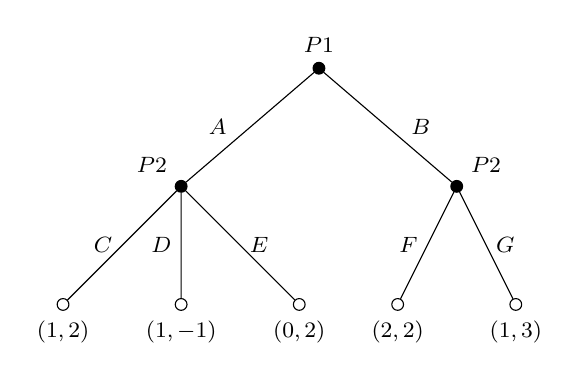
\begin{tikzpicture}[scale=1,font=\footnotesize]
\tikzstyle{solid node}=[circle,draw,inner sep=1.5,fill=black]
\tikzstyle{hollow node}=[circle,draw,inner sep=1.5]
\tikzstyle{level 1}=[level distance=15mm,sibling distance=3.5cm]
\tikzstyle{level 2}=[level distance=15mm,sibling distance=1.5cm]
\tikzstyle{level 3}=[level distance=15mm,sibling distance=1cm]
\node(0)[solid node,label=above:{$P1$}]{}
child{node[solid node,label=above left:{$P2$}]{}
child{node[hollow node,label=below:{$(1,2)$}]{} edge from parent node[left]{$C$}}
child{node[hollow node,label=below:{$(1,-1)$}]{} edge from parent node[left]{$D$}}
child{node[hollow node,label=below:{$(0,2)$}]{} edge from parent node[right]{$E$}}
edge from parent node[left,xshift=-5]{$A$}
}
child{node[solid node,label=above right:{$P2$}]{}
child{node[hollow node,label=below:{$(2,2)$}]{} edge from parent node[left]{$F$}}
child{node[hollow node,label=below:{$(1,3)$}]{} edge from parent node[right]{$G$}}
edge from parent node[right,xshift=5]{$B$}
};
\end{tikzpicture}
\end{doccode}



You can get a quite similar (actually the same) result by using the \pkg{istgame} package.

\begin{doccode}{.4}
% istgame
\begin{istgame}[scale=1,font=\footnotesize]
\setistDecisionNodeStyle{4pt}
\xtdistance{15mm}{3.5cm}
\istroot(0){$P1$}
  \istb{A}[al]
  \istb{B}[ar]              \endist
\xtShowEndPoints[oval node]
\xtdistance{15mm}{1.5cm}
\istroot(1)(0-1)<135>{$P2$}
  \istb{C}[l]{(1,2)}
  \istb{D}[l]{(1,-1)}
  \istb{E}[r]{(0,2)}        \endist
\istroot(2)(0-2)<45>{$P2$}
  \istb{F}[l]{(2,2)}
  \istb{G}[r]{(1,3)}        \endist
\end{istgame}
\end{doccode}


The \pkg{istgame} package enhances simplicity and readability, and hence it is easy to reuse codes. You can easily read and modify game tree codes even if you go over them after a while.


\section{Game tree examples}

This section provides some examples of extensive games.
Before we start, let us change the default font size of the \env{istgame} environment by stating
|\setistgamefontsize{|\cmd{\footnotesize}|}| outside of the environment. (Right here!)

\setistgamefontsize{\footnotesize}

\subsection{Simple examples}

\begin{doccode}{.35}
\begin{istgame}[->,shorten >=1.3pt]
\setistmathTF*001
\xtdistance{15mm}{30mm}
\istroot(0)[initial node]{Child}
  \istb{Good}[above left]{(0,2)}
  \istb{Bad}[above right]
  \endist
\istroot(1)(0-2)<30>{Parent}
  \istb{Forgive}[above left]{(1,1)}
  \istb{Punish}[above right]{(-1,-1)}
  \endist 
\end{istgame}
\end{doccode}

\medskip 

%\begin{doccode}{.35}
%% sloped action labels
%\begin{istgame}[->]
%\setistmathTF*001 % action labels in italics
%\xtShowEndPoints
%\xtdistance{15mm}{30mm}
%\istroot(0)[initial node]{Child}
%  \istb{Good}[above,sloped]{(0,2)}
%  \istb{Bad}[above,sloped]
%  \endist
%\istroot(1)(0-2)<30>{Parent}
%  \istb{Forgive}[above,sloped]{(1,1)}
%  \istb{Punish}[above,sloped]{(-1,-1)}
%  \endist 
%\end{istgame}
%\end{doccode}
%
%\medskip 

\begin{doccode}{.35}
% dual sloped action labels (\istB)
\begin{istgame}
\setistmathTF*001 % action labels in italics
\xtShowArrows
\xtdistance{15mm}{30mm}
\istroot(0)[initial node]{Child}
  \istB{Good}[above,sloped]
       {$p$}[below, sloped]{(0,2)}
  \istB{Bad}[above,sloped]
       {$1-p$}[below, sloped]
  \endist
\istroot(1)(0-2)<30>{Parent}
  \istB{Forgive}[above,sloped]
       {$q$}[below, sloped]{(1,1)}
  \istB{Punish}[above,sloped]
       {$1-q$}[below, sloped]{(-1,-1)}
  \endist 
\end{istgame}
\end{doccode}

\medskip 

\begin{doccode}{.35}
% IGT 218.1 (Osborne, 2004b)
\begin{istgame}[font=\normalsize]
\xtdistance{10mm}{20mm}
  \istroot(0){Vote}
  \istb{a}[al]{x}
  \istb{b}[ar]
  \endist
\istroot(1)([yshift=-1.5em]0-2){Vote}
  \istb{c}[al]{y}
  \istb{d}[ar]{z}
  \endist
\end{istgame}
\end{doccode}

\medskip

\begin{doccode}{.35}
% information set
\begin{istgame}
\xtdistance{10mm}{30mm}
\istroot(0){1}
  \istb{L}[al]   \istb{R}[ar] 
  \endist
\xtdistance{7mm}{15mm}
\istroot(1a)(0-1)
  \istb{a}[al]{1,0} 
  \istb{b}[ar]{2,3}  
  \endist
\istroot(1b)(0-2)
  \istb{c}[al]{0,1}   \istb{d}[ar]{-1,0} 
  \endist
\xtInfoset(1a)(1b){2}
\end{istgame}
\end{doccode}

\medskip

\begin{doccode}{.35}
% information set
\begin{istgame}
\xtShowEndPoints[oval node]
\xtdistance{10mm}{30mm}
\istroot(0){1}
  \istb{L}[al]   \istb{R}[ar] 
  \endist
\xtdistance{7mm}{15mm}
\istroot(1a)(0-1)
  \istb{a}[al]{1,0}   \istb{b}[ar]{2,3}  
  \endist
\istroot(1b)(0-2)
  \istb{c}[al]{0,1}   \istb{d}[ar]{-1,0} 
  \endist
\xtInfoset[bend left=30](1a)(1b){2}
\end{istgame}
\end{doccode}

\medskip 

\begin{doccode}{.35}
% (oval) information set
\begin{istgame}
\xtdistance{15mm}{30mm}
\istroot[-135](0)[initial node]<0>{1}
  \istb{A}[a]{(2,2)}[l]  \istb{D}[r]  
  \endist 
\istroot(1)(0-2)<left>{1}
  \istb{L}[al]    \istb{R}[ar]  
  \endist 
\xtInfosetO(1-1)(1-2){2}
\xtdistance{10mm}{20mm}
\istroot(2)(1-1)
  \istb{\ell}[al]{(4,2)}  \istb{r}[ar]{(1,1)}
  \endist 
\istroot(3)(1-2)
  \istb{\ell}[al]{(3,2)}  \istb{r}[ar]{(0,3)}
  \endist 
\end{istgame}
\end{doccode}


\subsection{A game tree with a strategic game}

\begin{doccode}{.35}
\DeclareExpandableDocumentCommand\xcol{O{c|}m}
  {\multicolumn{1}{#1}{\ensuremath{#2}}}
\def\strategicgame{%
  \begin{tabular}  {c|c|c|}
  \xcol[c]{~} & \xcol[c]{B} & \xcol[c]{S} 
                                \\\cline{2-3}
  $B$   & $3,1$     & $0,0$     \\\cline{2-3}
  $S$   & $0,0$     & $1,3$     \\\cline{2-3}
  \end{tabular}
}

\begin{istgame}
\setistmathTF*001
\xtdistance{10mm}{40mm}
\istroot(0)[initial node]{1}
  \istb{Book}[al]{2,2} \istb{Concert}[ar] \endist
\xtPayoff(0-2){\strategicgame}[below,xshift=-7pt]
\end{istgame}
\end{doccode}


%\clearpage
\subsection{Larger game trees with information sets}

\begin{doccode}[text above listing]
\begin{istgame}
\xtShowEndPoints
\xtdistance{10mm}{40mm}
\istroot(0)[initial node]{1}  \istb  \istb  \istb  \endist
\xtdistance{10mm}{10mm}
\istroot(1)(0-1)              \istb  \istb  \istb  \endist
\istroot(2)(0-2)              \istb  \istb  \istb  \endist
\xtdistance{10mm}{20mm}
\istroot(3)(0-3)              \istb  \istb  \endist
\xtdistance{10mm}{7mm}
\istroot(a)(1-3){3}           \istb  \istb  \istb  \endist
\xtdistance{10mm}{14mm}
\istroot(b)(2-3)              \istb  \istb  \endist
\istroot(c)(3-1){2}           \istb  \istb  \endist
\istroot(d)(3-2){2}           \istb  \istb  \endist
\xtInfosetO[fill=red!20](0)(0)
\xtInfoset(1)(2){2} 
\xtCInfosetO[fill=blue!20](a)(a)
\setxtinfosetstyle{blue,thick,dashed}
\xtInfosetO(b)(3){3}
\setxtinfosetstyle % restore defaults
\xtCInfosetO(d)(d)
\end{istgame}
\end{doccode}


\begin{doccode}[text above listing]
\begin{istgame}[scale=.8]
\useasboundingbox (-7,-3) rectangle (7,.5);
\xtdistance{10mm}{40mm}
\istroot(0)[initial node]{1}  \istb  \istb  \istb  \istb \endist
\xtdistance{10mm}{10mm}
\istroot(1)(0-1)     \istb  \istb  \istb  \endist
\istroot(2)(0-2)  \istb  \istb  \istb  \endist
\xtdistance{10mm}{20mm}
\istroot(3)(0-3)  \istb  \istb  \endist
\istroot(4)(0-4)  \istb  \istb  \endist
\xtdistance{10mm}{7mm}
\istroot(a)(1-3)  \istb  \istb  \istb  \endist
\istroot(b)(2-3)  \istb  \istb  \endist
\istroot(c)(3-1)  \istb  \istb  \istb  \endist
\xtCInfosetO[fill=red!20](1)!.4!(3){2} 
\xtInfosetO(2)(2){1}[above]
\setxtinfosetlayer{behind}
\xtCInfoset[blue,thick,dashed](a)(c)<.85>{3}[below]
\setxtinfosetlayer % restore default layer (behind)
\xtCInfosetO[fill=blue!20](b)(4)<.7>{2}
\end{istgame}
\end{doccode}


\subsection{A continuum of branches}

\begin{doccode}{.25}
\begin{istgame}[font=\scriptsize]
\cntmdistance*{8mm}{16mm}
\cntmpreset*[dashed]{.7} % white triangle
\istrootcntm(0)(0,0){1}  \istb{x}[r]  \endist
\istroot(1)(0-1)<[label distance=-3pt]120>{2}
  \istb{Y}[al]{x,1-x}    \istb{N}[ar] \endist
\cntmpreset % restore defaults
\istrootcntm(2)(1-2){2}  \istb{y}[r]  \istbm  \endist
\istroot(3)(2-1)<[label distance=-3pt]120>{1}
  \istb[]{Y}[al]{1-y,y}  \istb{N}[ar] \endist
\end{istgame}
\end{doccode}

%\medskip

\begin{doccode}{.25}
\begin{istgame}[font=\scriptsize]
\cntmdistance*{8mm}{16mm}
\istrootcntmA(0)(0,0){1} \istbA{x}[r]  \endist
\cntmAInfoset(0)
\istroot(1)(0-1)<[label distance=-3pt]120>{2}
  \istb{Y}[al]{x,1-x}    \istb{N}[ar]  \endist
\istrootcntmA(2)(1-2){2} \istbA{y}[r]  \endist
\cntmAInfosetO[fill=blue!20](2)
\istroot(3)(2-1)<[label distance=-3pt]120>{1}
  \istb[]{Y}[al]{1-y,y}  \istb{N}[ar]  \endist
\end{istgame}
\end{doccode}


\leavevmode
\vfill

\href{https://economics.stackexchange.com/questions/16465/how-to-visually-present-a-simultaneous-game-with-continuous-strategies/33039#33039}{\sourcelink{how-to-visually-present-a-simultaneous-game-with-continuous-strategies}}

\xbigskip1

\begin{doccode}{.4}
\DeclareDocumentCommand\vpay{ m }
{\begin{matrix} #1 \end{matrix}}

\begin{istgame}[scale=1.5,font=\scriptsize]
\cntmApreset{.9}
\cntmdistance{15mm}{20mm}
\istrootcntmA(0)[null node]{1}
  \istbA(.977)[->,thick]{q_1}[r]
  \istbm
  \endist
\cntmAInfosetO[thick,dashed](0)[-11](2em)
\istrootcntmA(1)(0-1)[null node]<180>{2}
  \istbm
  \istbA(.977)[->,thick]{q_2}[r]
    {\vpay{\pi_1(q_1,q_2)\\\pi_2(q_1,q_2)}}
  \endist
\end{istgame}
\end{doccode}

\vfill

\href{https://economics.stackexchange.com/questions/16465/how-to-visually-present-a-simultaneous-game-with-continuous-strategies/33039#33039}{\sourcelink{how-to-visually-present-a-simultaneous-game-with-continuous-strategies}}

\xbigskip1

\begin{doccode}{.4}
\DeclareDocumentCommand\vpay{ m }
{\begin{matrix} #1 \end{matrix}}

\begin{istgame}
\xtdistance{15mm}{40mm}
\cntmdistance{15mm}{30mm}
\cntmApreset[draw=none]{1}[red!50,opacity=.2]
\istroot(0){Challenger}
  \istb{In}[al]  \istb{Out}[ar]  \endist
\cntmAistb[draw=none]
\istrootcntmA(1)(0-1)<135>{Incumbent}
  \istbA{q_I}[left]  \endist
\cntmAInfosetO(1)
\cntmAistb[draw=none]
\istrootcntmA(2)(0-2)<45>{Incumbent}
  \istbA*{q_I}[left]
    {\vpay{\pi_C(0,q_I)\\\pi_I(0,q_I)}}
  \endist
\cntmApreset[draw=none]{1}[blue!50,opacity=.2]
\cntmAistb[draw=none]
\istrootcntmA(3)(1-1)<180>{Challenger}
  \istbA*{q_C}[midway,left]
    {\vpay{\pi_C(q_C,q_I)\\ \pi_I(q_C,q_I)}}
  \endist
\end{istgame}
\end{doccode}

\vfill

\clearpage
\subsection{Tic-tac-toe (sketch)}

% tic-tac-toe
\begin{doccode}[text above listing]
% tic-tac-toe (sketch)
\begin{istgame}[scale=1.8,font=\tiny]
\xtdistance{20mm}{7mm}
\istroot(0) \istb \istb \istb \istb \istb \istb{\dots} \istb \istb \istb{9}[r] \endist
\foreach \x in {1,...,4}
{\xtActionLabel(0)(0-\x){\x}[l]}
\xtdistance{10mm}{3mm}
\istroot(a1)(0-1) \istb{2}[l] \istb \istb \istb \istb \istb \istb \istb{9}[r] \endist
\istroot(a7)(0-7) \istb{1}[l] \istb \istb \istb \istb \istb \istb \istb{9}[r] \endist
\xtdistance{10mm}{2mm}
\istroot(A)(a1-3) \istb{2}[l] \istb \istb \istb \istb \istb \istb{9}[r] \endist
\istroot(B)(a1-8) \istb{2}[l] \istb \istb \istb \istb \istb \istb{8}[r] \endist
\istroot(C)(a7-8) \istb{1}[l] \istb \istb \istb \istb \istb \istb{8}[r] \endist
\istroot(Bx)(B-7) \istb{2}[l] \istb \istb \istb \istb \istb{7}[r] \endist
\istroot(By)(Bx-1) \istb{3}[l] \istb \istb \istb \istb{7}[r]  \endist
\istroot(Bz)(By-1) \istb{4}[l] \istb \istb \istb{7}[r]  \endist
\xtPayoff(Bz-4){\vdots}    \xtPayoff(Bz-4){\cdots}[right,xshift=10pt]
\end{istgame}
\end{doccode}


%\clearpage
\subsection{Selten's horse}

\begin{doccode}{.4}
% Selten's horse: IGT 331.2 (Osborne, 2004b)
\begin{istgame}
\xtdistance{8mm}{16mm}
\istroot[-45](0)[initial node]{1}
  \istb{D}[r]
  \istb<grow=east,level distance=30mm>{C}[a]
  \endist
\istroot(1)(0-1)+10mm..20mm+
  \istb{L}[al]{3,3,2}
  \istb{R}[ar]{0,0,0}
  \endist
\istroot[-45](a)(0-2){2}
  \istb{d}[r]
  \istb<grow=0,level distance=20mm>{c}[a]{1,1,1}[r]
  \endist
\istroot(a1)(a-1)+10mm..20mm+
  \istb{L}[al]{4,4,0}
  \istb{R}[ar]{0,0,1}
  \endist
\xtInfoset(1)(a1){3}
\end{istgame}
\captionof{figure}{IGT 331.2}
\end{doccode}


\subsection{Centipede game}

\begin{doccode}[text above listing]
% centipede
\begin{istgame}[scale=1.5]
\setistmathTF*001
\setistgrowdirection{south east}
\xtdistance{10mm}{20mm}
\istroot(0)[initial node]{1}
  \istb{Take}[r]{(2,0)}[b]  \istb{Pass}[a]  \endist
\istroot(1)(0-2){2}
  \istb{Take}[r]{(1,3)}[b]  \istb{Pass}[a]  \endist
\istroot(2)(1-2){1}
  \istb{Take}[r]{(4,2)}[b]  \istb{Pass}[a]  \endist
\xtInfoset(2-2)([xshift=5mm]2-2)
%-------------
\istroot(3)([xshift=5mm]2-2){2}
  \istb{Take}[r]{(97,99)}[b]  \istb{Pass}[a]  \endist
\istroot(4)(3-2){1}
  \istb{Take}[r]{(100,98)}[b]  \istb{Pass}[a]  \endist
\istroot(5)(4-2){2}
  \istb{Take}[r]{(99,101)}[b]  \istb{Pass}[a]{(100,100)}[r]  \endist
\end{istgame}
\end{doccode}


%\clearpage
\subsection{Poker game}

% poker
\begin{doccode}[text above listing]
% poker: growing south
\begin{istgame}[scale=1.7]
\setistmathTF*001
\xtShowEndPoints
\xtdistance{15mm}{30mm}
\istroot(0)[chance node]{N}
  \istB{Black}[al]{$\frac12$}[br]
  \istB{Red}[ar]{$\frac12$}[bl]
  \endist
\xtdistance{15mm}{30mm}
\istroot(1-1)(0-1){1}
  \istbA(.5)<grow=-135>{Fold}[al]{1,-1}
  \istb{Raise}[ar]
  \endist
\xtdistance{10mm}{20mm}
\istroot(1)(1-1-2)
  \istb{Pass}[al]{1,-1}
  \istb{Meet}[ar]{2,-2}
  \endist
\xtdistance{15mm}{30mm}
\istroot(1-2)(0-2){1}
  \istbA(.5)<grow=-135>{Fold}[al]{-1,1}
  \istb{Raise}[ar]
  \endist
\xtdistance{10mm}{20mm}
\istroot(2)(1-2-2){}
  \istb{Pass}[al]{1,-1}
  \istb{Meet}[ar]{-2,2}
  \endist
\xtInfoset(1)(2){2}
\end{istgame}
\end{doccode}


\subsection{Poker game: growing to the right}
\label{p:poker-right}

\begin{doccode}[text above listing]
% poker: growing east -- counterclockwise
\begin{istgame}[scale=1.3]
\setistmathTF*001
\setistgrowdirection{0}   % default grow-direction is 'east' from now on
\xtdistance{15mm}{30mm}
\istroot(0)[chance node]<left>{N}
  \istB{Black}[bl]{$\frac12$}[ar]
  \istB{Red}[al]{$ \frac12$}[br]
  \endist
\xtdistance{15mm}{30mm}
\istroot(1-1)(0-1)<left>{1}
  \istb<grow=-45,level distance=10mm>{Fold}[bl]{1,-1}
  \istb{Raise}[al]
  \endist
\xtdistance{12mm}{24mm}
\istroot(1)(1-1-2)
  \istb{Pass}[bl]{1,-1}
  \istb{Meet}[al]{2,-2}
  \endist
\xtdistance{15mm}{30mm}
\istroot(1-2)(0-2)<left>{1}
  \istb<grow=-45,level distance=10mm>{Fold}[bl]{-1,1}[[xshift=5pt]below]
  \istb{Raise}[al]
  \endist
\xtdistance{12mm}{24mm}
\istroot(2)(1-2-2)
  \istb{Pass}[bl]{1,-1}
  \istb{Meet}[al]{-2,2}
  \endist
\xtCInfosetO[fill=blue!20](1-1-2)(1-2-2){2}
\end{istgame}
\end{doccode}

\begin{doccode}[text above listing]
% poker: growing east -- clockwise (swap version)
\begin{istgame}[scale=1.3]
\setistmathTF*001
\setistgrowdirection'{0}   % \setistgrowdirection'
\xtdistance{15mm}{30mm}
\istroot(0)[chance node]<left>{N}
  \istB{Black}[al]{$\frac12$}[br]
  \istB{Red}[bl]{$\frac12$}[ar]
  \endist
\xtdistance{15mm}{30mm}
\istroot(1-1)(0-1)<left>{1}
  \istb<grow=45,level distance=10mm>{Fold}[al]{1,-1}
  \istb{Raise}[bl]
  \endist
\xtdistance{12mm}{24mm}
\istroot(1)(1-1-2)
  \istb{Pass}[al]{1,-1}
  \istb{Meet}[bl]{2,-2}
  \endist
\xtdistance{15mm}{30mm}
\istroot(1-2)(0-2)<left>{1}
  \istb<grow=45,level distance=10mm>{Fold}[al]{-1,1}
  \istb{Raise}[bl]
  \endist
\xtdistance{12mm}{24mm}
\istroot(2)(1-2-2)
  \istb{Pass}[al]{1,-1}
  \istb{Meet}[bl]{-2,2}
  \endist
\xtInfosetO[fill=red!20](1-1-2)(1-2-2){2}
\end{istgame}
\end{doccode}

\subsection{Signaling games}

\begin{doccode}[text above listing,halign lower=center]
% signaling game: IGT 337.1 (Osborne, 2004b)
\begin{istgame}
\setistgrowdirection'{right}
% game start: choice of chance
\xtdistance{20mm}{20mm}
\istroot(0)[chance node]<180>{Chance}
  \istB<grow=north>{H}[l]{\pi}[r]  \istB<grow=south>{L}[l]{1-\pi}[r]  \endist
\istroot(H0)(0-1)<180>{F}
  \istb{(p_1,E)}[a]  \endist
\istroot(L0)(0-2)<180>{F}
  \istb{(p_1,E)}[a]  \endist
\setistmathTF*001
\cntmdistance*{10mm}{20mm}{8mm}
% subtree after H is chosen
\istroot(H)(H0-1)
  \istb{Buy}[br]  \istb{Refrain}[ar]{-E,0}  \endist
\istrootcntm(H1)(H-1)
  \istb{$p_2^H$}[b]  \istbm  \endist
\istroot(CH)(H1-1)<[label distance=-4pt]135>{C}
  \istb{Buy}[br]{p_1-E-c_H+p_2^H-c_H, 2H-p_1-p_2^H}
  \istb{Refrain}[ar]{p_1-E-c_H, H-p_1}
  \endist
% subtree after L is chosen
\istroot(L)(L0-1)
  \istb{Buy}[br]  \istb{Refrain}[ar]{-E,0}  \endist
\istrootcntm(L1)(L-1)
  \istbm  \istb{$p_2^L$}[a]  \endist
\istroot(CL)(L1-2)<[label distance=-4pt]-135>{C}
  \istb{Buy}[br]{p_1-E-c_L+p_2^L-c_L, 2L-p_1-p_2^L}
  \istb{Refrain}[ar]{p_1-E-c_L, L-p_1}
  \endist
\xtInfoset(H)(L){C}[left]
\end{istgame}
\end{doccode}

\xbigskip2

\begin{doccode}{.5}
% signaling game
\begin{istgame}[scale=1.3]
\xtdistance{20mm}{20mm}
\istroot(0)[chance node]{$c$}
  \istb<grow=left>{\frac12}[a]
  \istb<grow=right>{\frac12}[a]
  \endist
\xtdistance{10mm}{20mm}
\istroot(1)(0-1)<180>{1}
  \istb<grow=north>{a}[l]
  \istb<grow=south>{b}[l]
  \endist
\istroot(2)(0-2)<0>{1}
  \istb<grow=north>{a}[r]
  \istb<grow=south>{b}[r]
  \endist
\istroot'[north](a1)(1-1)
  \istb{L}[bl]{-1,0}
  \istb{R}[br]{0,-1}
  \endist
\istroot(b1)(1-2)
  \istb{L}[al]{2,0}
  \istb{R}[ar]{0,2}
  \endist
\istroot(a2)(2-2)
  \istb{L}[al]{3,0}
  \istb{R}[ar]{0,3}
  \endist
\istroot'[north](b2)(2-1)
  \istb{L}[bl]{1,0}
  \istb{R}[br]{0,1}
  \endist
\xtInfoset(a1)(b2){2}
\xtInfoset(b1)(a2){2}
\end{istgame}
\end{doccode}



\clearpage
\section{Selected examples from \texttt{tex.stackexchange.com}}

In this section |\setistgamefontsize{|\cmd{\normalsize}|}|.
\setistgamefontsize{\normalsize}

\subsection{Subgames: \protect\CMD{\xtSubgameBox}}

\vfill

\href{https://tex.stackexchange.com/questions/482883/game-theory-subgame-box/488559#488559}{\sourcelink{game-theory-subgame-box}}

\vfill

\begin{doccode}[text above listing]
\begin{istgame}
\xtShowEndPoints
\xtdistance{25mm}{70mm}
\istrooto(0){Firm 1}
  \istb{BIG}[al]  \istb{small}[ar]  \endist
\xtdistance{25mm}{35mm}
\istrooto(1)(0-1){Firm 2}
  \istb{Low}[al]  \istb{High}[ar]  \endist
\istrooto(2)(0-2){Firm 2}  \istb{low}[al]  \istb{high}[ar]  \endist
\xtdistance{20mm}{10mm}
\istrooto(a)(1-1){Firm 1}
  \istb{L}[l]{\parbox{1em}{$u_1$\\$u_2$}}  \istb{H}[r]  \endist
\istrooto(b)(1-2){Firm 1}
  \istb{L}[l]  \istb{H}[r]  \endist
\istrooto(c)(2-1){Firm 1}
  \istb{l}[l]  \istb{h}[r]  \endist
\istrooto(d)(2-2){Firm 1}
  \istb{l}[l]  \istb{h}[r]  \endist
\setxtinfosetstyle{dashed}
\xtInfoset(a)(b)
\xtInfoset(c)(d)
\xtSubgameBox([yshift=-2ex]1){(a-1)(b-2)}[inner ysep=7ex]
\xtSubgameBox([yshift=-2ex]2){(c-1)(d-2)}[inner ysep=7ex]
\end{istgame}
\end{doccode}

\vfill

\clearpage
\subsection{Information sets: \protect\CMD{\xtInfosetO}, \protect\CMD{\xtCInfosetO}, and \protect\CMD{\cntmAInfosetO}}

\vfill

\href{https://tex.stackexchange.com/questions/430077/game-theory-forest-tree-dashed-ellipse-between-various-nodes/478240#478240}{\sourcelink{game-theory-forest-tree-dashed-ellipse-between-various-nodes}}

\vfill

\begin{doccode}[text above listing]
\begin{istgame}[scale=1.2]
\setistgrowdirection'{east}
\tikzset{oval node/.style={ellipse node,draw=none}}
\tikzset{move/.style={red,fill=white}}
\xtdistance{25mm}{25mm}
\istroot(0)[null node]<180>{1}+25mm..40mm+
  \istb{1}[move] \istb{2}[move] \endist
\istrooto(1)(0-1){2}
  \istb{1}[move] \istb{2}[move] \endist
\istrooto(2)(0-2){2}
  \istb{1}[move] \istb{2}[move]{(-1,1)} \endist
\istrooto(3)(1-1){1}
  \istb{1}[move] \istb{2}[move]{(-1,1)} \endist
\istrooto(4)(1-2){1}
  \istb{1}[move]{(-1,1)} \endist
\istrooto(5)(2-1){1}
  \istb{1}[move]{(-1,1)} \endist
\istrooto(6)(3-1){2}
  \istb{1}[move]{(-1,1)} \endist
\setxtinfosetlayer{main}
\xtInfosetO[dashed,thick](3)(4)(1.5em)
\xtInfosetO[ellipse,dashed,thick](2)(5)(2em)
\end{istgame}
\end{doccode}

\vfill

\clearpage
\href{https://tex.stackexchange.com/questions/497214/follow-up-drawing-game-tree-with-curved-informational-sets-and-several-nodes-u/497333#497333}{\sourcelink{drawing-game-tree-with-curved-informational-sets}}

\begin{doccode}[text above listing]
\begin{istgame}[scale=.55,font=\footnotesize]
\setistmathTF*001
% top part
\xtdistance{25mm}{120mm}
\istroot(0)[chance node]{Nature} \istb \istb  \endist
\xtdistance{25mm}{50mm}
\istroot(A)(0-1)           \istb  \endist
\istroot(B)(0-2)           \istb  \endist
% left part
\xtdistance{25mm}{60mm}
\istroot(A0)(A-1)<180>{2}  \istb  \istb  \endist
\xtdistance{25mm}{30mm}
\istroot(A1)(A0-1)         \istb  \istb  \endist
\istroot(A2)(A0-2)         \istb  \istb  \endist
\xtdistance{25mm}{15mm}
\istroot(A3)(A1-1)<180>{2} \istb{G}[l]  \istb{S}[r]  \endist
\istroot(A4)(A1-2)<180>{2} \istb{G}[l]  \istb{S}[r]  \endist
\istroot(A5)(A2-1)<180>{2} \istb{G}[l]  \istb{S}[r]  \endist
\istroot(A6)(A2-2)<180>{2} \istb{G}[l]  \istb{S}[r]  \endist
% right part
\xtdistance{25mm}{60mm}
\istroot(B0)(B-1)<180>{2}  \istb  \istb  \endist
\xtdistance{25mm}{30mm}
\istroot(B1)(B0-1) \istb   \istb  \endist
\istroot(B2)(B0-2) \istb   \istb  \endist
\xtdistance{25mm}{15mm}
\istroot(B3)(B1-1)<180>{2} \istb{G}[l]  \istb{S}[r]  \endist
\istroot(B4)(B1-2)<180>{2} \istb{G}[l]  \istb{S}[r]  \endist
\istroot(B5)(B2-1)<180>{2} \istb{G}[l]  \istb{S}[r]  \endist
\istroot(B6)(B2-2)<180>{2} \istb{G}[l]  \istb{S}[r]  \endist
% information sets
\setxtinfosetstyle{dashed}
\xtInfosetO[fill=black!15](A)(B){1}
\xtCInfosetO[blue,fill=blue!15](A1)!.35!(B1)<1.15>{1}
\xtCInfosetO[red,fill=red!15](A2)!.5!(B2)<.75>{1}
\end{istgame}
\end{doccode}


\href{https://tex.stackexchange.com/questions/622934/how-to-design-a-game-in-a-tree/623249#623249}{\sourcelink{how-to-design-a-game-in-a-tree}}

\vfill

%\begin{doccode}[text only]
\begin{istgame}[scale=1.5]
\setistgrowdirection'{east}
%% root
\xtdistance{20mm}{32mm}
\istroot(0)[chance node]{0}
  \istb  \istb  \istb  \istb  \endist
%% extending branches
\istroot(0a)(0-1)[null node]
  \istb{\frac13(TL)}[above,near start] \endist
\istroot(0b)(0-2)[null node]
  \istb{\frac13(BL)}[above,near start] \endist
\istroot(0c)(0-3)[null node]
  \istb{\frac13(TR)}[below,near start] \endist
\istroot(0d)(0-4)[null node]
  \istb{0(BR)}[below,near start] \endist
%\xtShowEndPoints    
%% player I
\xtdistance{15mm}{16mm}
\istroot(1a)(0a-1)
  \istb{T_1}[a]  \istb{B_1}[b]  \endist
\istroot(1b)(0b-1)
  \istb{T_2}[a]  \istb{B_2}[b]  \endist
\istroot(1c)(0c-1)
  \istb{T_1}[a]  \istb{B_1}[b]  \endist
\istroot(1d)(0d-1)
  \istb{T_2}[a]  \istb{B_2}[b]  \endist
\xtdistance{15mm}{8mm}
%% player II
\istroot(2Aa)(1a-1)
  \istb{L_1}[a]{6,6}  \istb{R_1}[b]{2,7}  \endist
\istroot(2Ab)(1a-2)
  \istb{L_1}[a]{7,2}  \istb{R_1}[b]{0,0}  \endist
\istroot(2Ac)(1b-1)
  \istb{L_1}[a]{6,6}  \istb{R_1}[b]{2,7}  \endist
\istroot(2Ad)(1b-2)
  \istb{L_1}[a]{7,2}  \istb{R_1}[b]{0,0}  \endist
\istroot(2Ba)(1c-1)
  \istb{L_2}[a]{6,6}  \istb{R_2}[b]{2,7}  \endist
\istroot(2Bb)(1c-2)
  \istb{L_2}[a]{7,2}  \istb{R_2}[b]{0,0}  \endist
\istroot(2Bc)(1d-1)
  \istb{L_2}[a]{6,6}  \istb{R_2}[b]{2,7}  \endist
\istroot(2Bd)(1d-2)
  \istb{L_2}[a]{7,2}  \istb{R_2}[b]{0,0}  \endist
% information sets
\xtInfosetO(0)(0)
\xtCInfosetO[fill=red!20,fill opacity=.3](1a)!.4!(1c)<1.2>{I}
\xtCInfosetO[fill=blue!20,fill opacity=.3](1b)!.6!(1d)<1.15>{I}
\xtInfosetO(2Aa)(2Ad){II}
\xtInfosetO(2Ba)(2Bd){II}

\end{istgame}
%\end{doccode}

\vfill

\clearpage

\leavevmode
\vfill

\begin{doccode}[listing only]
\begin{istgame}[scale=1.5]
\setistgrowdirection'{east}
%% root
\xtdistance{20mm}{32mm}
\istroot(0)[chance node]{0}
  \istb  \istb  \istb  \istb  \endist
%% extending branches
\istroot(0a)(0-1)[null node]
  \istb{\frac13(TL)}[above,near start] \endist
\istroot(0b)(0-2)[null node]
  \istb{\frac13(BL)}[above,near start] \endist
\istroot(0c)(0-3)[null node]
  \istb{\frac13(TR)}[below,near start] \endist
\istroot(0d)(0-4)[null node]
  \istb{0(BR)}[below,near start] \endist
%\xtShowEndPoints    
%% player I
\xtdistance{15mm}{16mm}
\istroot(1a)(0a-1)
  \istb{T_1}[a]  \istb{B_1}[b]  \endist
\istroot(1b)(0b-1)
  \istb{T_2}[a]  \istb{B_2}[b]  \endist
\istroot(1c)(0c-1)
  \istb{T_1}[a]  \istb{B_1}[b]  \endist
\istroot(1d)(0d-1)
  \istb{T_2}[a]  \istb{B_2}[b]  \endist
\xtdistance{15mm}{8mm}
%% player II
\istroot(2Aa)(1a-1)
  \istb{L_1}[a]{6,6}  \istb{R_1}[b]{2,7}  \endist
\istroot(2Ab)(1a-2)
  \istb{L_1}[a]{7,2}  \istb{R_1}[b]{0,0}  \endist
\istroot(2Ac)(1b-1)
  \istb{L_1}[a]{6,6}  \istb{R_1}[b]{2,7}  \endist
\istroot(2Ad)(1b-2)
  \istb{L_1}[a]{7,2}  \istb{R_1}[b]{0,0}  \endist
\istroot(2Ba)(1c-1)
  \istb{L_2}[a]{6,6}  \istb{R_2}[b]{2,7}  \endist
\istroot(2Bb)(1c-2)
  \istb{L_2}[a]{7,2}  \istb{R_2}[b]{0,0}  \endist
\istroot(2Bc)(1d-1)
  \istb{L_2}[a]{6,6}  \istb{R_2}[b]{2,7}  \endist
\istroot(2Bd)(1d-2)
  \istb{L_2}[a]{7,2}  \istb{R_2}[b]{0,0}  \endist
% information sets
\xtInfosetO(0)(0)
\xtCInfosetO[fill=red!20,fill opacity=.3](1a)!.4!(1c)<1.2>{I}
\xtCInfosetO[fill=blue!20,fill opacity=.3](1b)!.6!(1d)<1.15>{I}
\xtInfosetO(2Aa)(2Ad){II}
\xtInfosetO(2Ba)(2Bd){II}

\end{istgame}
\end{doccode}

\vfill
\vfill
\vfill

\clearpage

\subsection{Continuum of moves: \protect\CMD{\istrootcntm} and \protect\CMD{\istrootcntmA}}

\leavevmode
\vfill

\href{https://tex.stackexchange.com/questions/468397/draw-tree-in-tikz/468703#468703}{\sourcelink{draw-tree-in-tikz}}

\vfill

\begin{doccode}[text above listing]
\begin{istgame}[scale=.8,font=\scriptsize]
% presets
\tikzset{odd node/.style={decision node,minimum size=6pt}}
\tikzset{even node/.style={oval node,fill=cyan!50,minimum size=6pt}}
% game tree 
\cntmdistance*{20mm}{35mm}
\cntmpreset*[densely dashed]{.6}
\istrootcntm(1a)[odd node]<15>{$x_1$}
  \istb{(a^0,1-a^0)}[right,near end] \endist
\istroot(2)(1a-1)[even node]<-90>{$x_2$}
  \istb{acc}[al]{\left(a^0,1-a^0\right)} 
  \istb{not}[ar] 
  \endist
\istrootcntm(2a)(2-2)[even node]<0>{$x_3$}
  \istb{(a^1,1-a^1)}[right,near end] \endist
\istroot(3)(2a-1)[odd node]<-90>{$x_4$}
  \istb{acc}[al]{\left(\delta_1 a^1,\delta_2(1-a^1)\right)} 
  \istb{not}[ar] 
  \endist
\istrootcntm(3a)(3-2)[odd node]<0>{$x_5$}
  \istb{(a^2,1-a^2)}[right,near end] \endist
\istroot(4)(3a-1)[even node]<-90>{$x_6$}
  \istb{acc}[al]{\left((\delta_1)^2a^2,(\delta_2)^2(1-a^2)\right)} 
  \istb{not}[ar]{(0,0)} 
  \endist
\end{istgame}
\end{doccode}

\vfill

\clearpage

\vfill

\href{https://tex.stackexchange.com/questions/594222/tikz-game-tree-help-drawing/594552#594552}{\sourcelink{tikz-game-tree-help-drawing}}

\vfill

\begin{doccode}[text above listing]
\begin{istgame}[scale=1.3]
% nodes
\tikzset{p1/.style={oval node,minimum size=3pt}}
\tikzset{p2/.style={oval node,fill=black,minimum size=3pt}}
% tree
\xtdistance{20mm}{45mm}
\cntmdistance{10mm}{20mm}
\istroot(1)[p1] \istb \istb \endist
\istrootcntmA(2a)(1-1)[p2] \istbA[draw=none] \endist
\istrootcntmA(2b)(1-2)[p2] \istbA[draw=none] \endist
\xtdistance{15mm}{30mm}
\istroot(1a)(2a-1)[p1] \istb \istb \endist
\istroot(1b)(2b-1)[p1] \istb \endist
\istrootcntmA(2c)(1a-1)[p2] \istbA[draw=none] \endist
\istrootcntmA(2d)(1a-2)[p2] \istbA[draw=none] \endist
\istrootcntmA(2e)(1b-1)[p2] \istbA[draw=none] \endist
\istroot(1c)(2c-1)[p1] \istb \endist
\istroot(1d)(2d-1)[p1] \istb \endist
\istroot(1e)(2e-1)[p1] \istb \endist
% information sets
\xtInfosetO[solid,thin,fill=blue!10](2a)(2b)
\xtInfosetO[solid,thin,fill=blue!10](2d)(2e)
\end{istgame}
\end{doccode}

\vfill

\clearpage

\vfill

\href{https://tex.stackexchange.com/questions/203052/a-gametree-with-variable-choices/472415#472415}{\sourcelink{a-gametree-with-variable-choices}}

\vfill

\begin{doccode}[text above listing]
\begin{istgame}[scale=1.3,semithick]
\tikzset{oval node/.style={box node,draw=none,minimum size=5mm}}
\cntmdistance*{20mm}{25mm}
\istrooto(0)[plain node]{Firm 1}+15mm..50mm+
  \istb \istb \endist
\setistmathTF111
\cntmApreset[dashed,thick]{.6}
\istrootocntmA(E2)(0-1){E_2}  \istb[thin]  \endist
\xtNode*(cntm-1){0}    \xtNode*(cntm-2){\infty}
\istrootocntmA(E3)(0-2){E_3}  \istb[thin]  \endist
\xtNode*(cntm-1){0}    \xtNode*(cntm-2){\infty}
\istrootocntmA(11)(E2-1){q_1}  \istb[thin]  \endist
\xtNode*(cntm-1){0}    \xtNode*(cntm-2){\infty}
\istrootocntmA(21)(E3-1){q_1}  \istb[thin]  \endist
\xtNode*(cntm-1){0}    \xtNode*(cntm-2){\infty}
\istrooto(3a)(11-1){q_2}  \istb[thin]  \endist
\xtNode*(3a-1){\big(\prod\big)_1^{c_2}\prod_2^c\prod_3^m}
\istrooto(3b)(21-1){q_3}  \istb[thin]  \endist
\xtNode*(3b-1){\big(\prod\big)_1^{c_3}\prod_2^m\prod_3^c}
\end{istgame}
\end{doccode}


\vfill

\clearpage



\subsection{Signaling games}

\leavevmode
\vfill

\href{https://tex.stackexchange.com/questions/594771/how-draw-this-game-in-tikz/610845#610845}{\sourcelink{how-draw-this-game-in-tikz}}

\vfill

\begin{doccode}[text above listing]
\begin{istgame}
\setistNewNodeStyle{solid node}[null node]
\setistmathTF001
\setxtshowarrows[thick]
\xtShowArrows
\xtHideEndPoints
% game start
\setistgrowdirection'{east}
\xtdistance{10mm}{40mm}
\istroot(0)[chance node]<[xshift=2mm]200>{Nature}
  \istb{[.5]1}[l]  \istb{[.5]2}[l]  \endist
% right part
\xtdistance{30mm}{20mm}
\istroot(Ra)(0-1)<-45>{$x_1$}  \istb{Average}[a] \endist
\istroot(Rb)(0-2)<45>{$x_2$}   \istb{Average}[b] \endist
\xtdistance{20mm}{20mm}
\istroot(T1a)(Ra-1)<-135>{$x_3$}
  \istb{Hunk}[above,sloped]{2,3}  \istb{Average}[below,sloped]{2,2}  \endist
\istroot(T1b)(Rb-1)<135>{$x_4$}
  \istb{Hunk}[above,sloped]{2,3}  \istb{Average}[below,sloped]{2,2}  \endist
\xtInfoset[dashed](0-1)(0-2){$h_G$}[l]
\xtInfosetOwner(0-1)(0-2){Gina}[r]
\xtInfoset[dashed](T1a)(T1b){$h_{T1}$}[l]
\xtInfosetOwner(T1a)(T1b){Tina}[r]
% left part
\setistgrowdirection{west}
\xtdistance{30mm}{20mm}
\istroot(La)(0-1) \istb{Hunk}[a] \endist
\istroot(Lb)(0-2) \istb{Hunk}[b] \endist
\xtdistance{20mm}{20mm}
\istroot(T2a)(La-1)<-45>{$x_5$}
  \istb{Hunk}[above,sloped]{3,0}  \istb{Average}[below,sloped]{3,2}  \endist
\istroot(T2b)(Lb-1)<45>{$x_6$}
  \istb{Hunk}[above,sloped]{0,3}  \istb{Average}[below,sloped]{3,2}  \endist
% information set
\xtInfoset[dashed](T2a)(T2b){$h_{T2}$}[r]
\xtInfosetOwner(T2a)(T2b){Tina}[l]
\end{istgame}
\end{doccode}

\vfill

\clearpage

\subsection{Cross out nodes}

\leavevmode
\vfill

\href{https://tex.stackexchange.com/questions/374600/problem-with-dashed-edges-and-cross-nodes/402407#402407}{\sourcelink{problem-with-dashed-edges-and-cross-nodes}}

\vfill

\begin{doccode}[text above listing]
\begin{istgame}
\setistNewNodeStyle{cross node}[cross out,ultra thick]{4pt}
\xtdistance{15mm}{55mm}
\istroot(1a){1.1}
  \istb{L_1}[al]  \istb{R_1}[ar]  \endist
\xtdistance{15mm}{27mm}
\istroot(2a)(1a-1)<135>{2.1}
  \istb[dashdotted]{l_1}[l]  \istb{r_1}[r]  \endist
\istroot(2b)(1a-2)<45>{2.2}
  \istb{l_2}[l]  \istb*{r_1}[r]  \endist
\xtdistance{15mm}{17mm}
\istroot(1b)(2a-1)[cross node]<135>{1.2}
  \istb[dashdotted]{L_2}[l]  \istb*[dashdotted]{R_2}[r]  \endist
\istroot(1c)(2a-2)<45>{1.3}
  \istb{L_3}[l]  \istb{R_3}[r]  \endist
\istroot(1d)(2b-1)<135>{1.4}
  \istb*{L_4}[l]  \istb{R_4}[r]  \endist
\xtShowEndPoints
\xtdistance{18mm}{10mm}
\istroot(2c)(1b-1)[cross node]<135>{2.3}
  \istb[dashdotted]{l_3}[l]  \istb[dashdotted]{r_3}[r]  \endist
\istroot(2d)(1c-1)<135>{2.4}
  \istb{l_4}[l]  \istb{r_4}[r]  \endist
\istroot(2e)(1c-2)<45>{2.5}
  \istb{l_5}[l]  \istb{r_5}[r]  \endist
\istroot(2f)(1d-2)<45>{2.6}
  \istb{l_6}[l]  \istb{r_6}[r]  \endist
\end{istgame}
\end{doccode}

\vfill

\clearpage

\subsection{Large game trees}

%\leavevmode
\vfill

\href{https://tex.stackexchange.com/questions/482040/game-theory-trees-solid-node-size/482610#482610}{\sourcelink{game-theory-trees-solid-node-siz}}

\vfill
\vfill
\vfill

%\begin{doccode}[text above listing]
\def\vpay#1#2{\begin{matrix}#1\\#2\end{matrix}}

\begin{istgame}[scale=.8,font=\footnotesize]
\xtShowEndPoints % solid nodes
\setistEllipseNodeStyle{6mm} % minimum circle size for players
\xtdistance{30mm}{30mm}
\istrooto(0){Nature}
  \istB{JQK}[l]{p_1}[left,near start,xshift=-5pt]
  \istB{JKQ}[l]{p}[left,near start]
  \istB{QJK}[l]{p}[left,near start]
  \istB{QJK}[r]{p}[right,near start]
  \istB{KJQ}[r]{p}[right,near start,xshift=5pt]
  \istB{KQJ}[r]{p}[right,near start,xshift=5pt]
  \endist
\xtdistance{25mm}{10mm}
\istrooto(1)(0-1){$P_1$}
  \istb{c}[l]{\vpay{-1}{1}} \istb<grow=-70,level distance=90mm>{r}[r] \endist
\istrooto(2)(0-2){$P_1$}
  \istb{c}[l]{\vpay{-1}{1}} \istb{r}[r] \endist
\istrooto(3)(0-3){$P_1$}
  \istb{r}[l] \istb{c}[r]{\vpay{-1}{1}} \endist
\istrooto(4)(0-4){$P_1$}
  \istb{c}[l]{\vpay{1}{-1}} \istb{r}[r] \endist
\istrooto(5)(0-5){$P_1$}
  \istb{r}[l] \istb{c}[r]{\vpay{1}{-1}} \endist
\istrooto(6)(0-6){$P_1$}
  \istb<grow=-110,level distance=90mm>{r}[l] \istb{c}[r]{\vpay{1}{-1}} \endist
\xtdistance{20mm}{10mm}
\istrooto(a)(2-2){$P_2$}
  \istb{f}[l]{\vpay{1}{-1}} \istb{c}[r]{\vpay{-2}{2}} \endist
\istrooto(b)(3-1){$P_2$}
  \istb{f}[l]{\vpay{1}{-1}} \istb{c}[r]{\vpay{-2}{2}} \endist
\istrooto(c)(4-2){$P_2$}
  \istb{f}[l]{\vpay{1}{-1}} \istb{c}[r]{\vpay{2}{-2}} \endist
\istrooto(d)(5-1){$P_2$}
  \istb{f}[l]{\vpay{1}{-1}} \istb{c}[r]{\vpay{2}{-2}} \endist
\xtdistance{28mm}{25mm}
\istrooto(A)(1-2){$P_2$}
  \istb[draw=red]{f}[l]{\vpay{1}{-1}} \istb[draw=blue]{c}[r]{\vpay{-2}{2}} \endist
\istrooto(B)(6-1){$P_2$}
  \istb[double]{r}[l]{\vpay{1}{-1}} \istb[ultra thick]{c}[r]{\vpay{2}{-2}} \endist
% information sets
\setxtinfosetstyle{dashed}
\xtInfoset(1)(2)
\xtInfoset(3)(4)
\xtInfoset(5)(6)
\xtInfoset(a)(b)
\xtInfoset(c)(d)
\xtInfoset(A)(B)
\end{istgame}
%\end{doccode}

\vfill
\vfill
\vfill

\clearpage

\leavevmode
\vfill

\begin{doccode}[listing only]
\def\vpay#1#2{\begin{matrix}#1\\#2\end{matrix}}

\begin{istgame}[scale=.8,font=\footnotesize]
\xtShowEndPoints % solid nodes
\setistEllipseNodeStyle{6mm} % minimum circle size for players
\xtdistance{30mm}{30mm}
\istrooto(0){Nature}
  \istB{JQK}[l]{p_1}[left,near start,xshift=-5pt]
  \istB{JKQ}[l]{p}[left,near start]
  \istB{QJK}[l]{p}[left,near start]
  \istB{QJK}[r]{p}[right,near start]
  \istB{KJQ}[r]{p}[right,near start,xshift=5pt]
  \istB{KQJ}[r]{p}[right,near start,xshift=5pt]
  \endist
\xtdistance{25mm}{10mm}
\istrooto(1)(0-1){$P_1$}
  \istb{c}[l]{\vpay{-1}{1}} \istb<grow=-70,level distance=90mm>{r}[r] \endist
\istrooto(2)(0-2){$P_1$}
  \istb{c}[l]{\vpay{-1}{1}} \istb{r}[r] \endist
\istrooto(3)(0-3){$P_1$}
  \istb{r}[l] \istb{c}[r]{\vpay{-1}{1}} \endist
\istrooto(4)(0-4){$P_1$}
  \istb{c}[l]{\vpay{1}{-1}} \istb{r}[r] \endist
\istrooto(5)(0-5){$P_1$}
  \istb{r}[l] \istb{c}[r]{\vpay{1}{-1}} \endist
\istrooto(6)(0-6){$P_1$}
  \istb<grow=-110,level distance=90mm>{r}[l] \istb{c}[r]{\vpay{1}{-1}} \endist
\xtdistance{20mm}{10mm}
\istrooto(a)(2-2){$P_2$}
  \istb{f}[l]{\vpay{1}{-1}} \istb{c}[r]{\vpay{-2}{2}} \endist
\istrooto(b)(3-1){$P_2$}
  \istb{f}[l]{\vpay{1}{-1}} \istb{c}[r]{\vpay{-2}{2}} \endist
\istrooto(c)(4-2){$P_2$}
  \istb{f}[l]{\vpay{1}{-1}} \istb{c}[r]{\vpay{2}{-2}} \endist
\istrooto(d)(5-1){$P_2$}
  \istb{f}[l]{\vpay{1}{-1}} \istb{c}[r]{\vpay{2}{-2}} \endist
\xtdistance{28mm}{25mm}
\istrooto(A)(1-2){$P_2$}
  \istb[draw=red]{f}[l]{\vpay{1}{-1}} \istb[draw=blue]{c}[r]{\vpay{-2}{2}} \endist
\istrooto(B)(6-1){$P_2$}
  \istb[double]{r}[l]{\vpay{1}{-1}} \istb[ultra thick]{c}[r]{\vpay{2}{-2}} \endist
% information sets
\setxtinfosetstyle{dashed}
\xtInfoset(1)(2)
\xtInfoset(3)(4)
\xtInfoset(5)(6)
\xtInfoset(a)(b)
\xtInfoset(c)(d)
\xtInfoset(A)(B)
\end{istgame}
\end{doccode}

\vfill
\vfill
\vfill

\clearpage


\subsection{Probability trees}

\vfill

\href{https://tex.stackexchange.com/questions/563364/draw-a-counting-tree-with-grow-right-and-then-placed-on-the-right-or-left-of-p/564322#564322}{\sourcelink{draw-a-counting-tree-with-grow-right-and-then-placed-on-the-right-or-left-of-p}}

\vfill

\begin{doccode}{.25}
\begin{istgame}[scale=.7]
\tikzset{oval node/.style={ellipse node,draw=none}}
\setistgrowdirection'{east}
\xtdistance{14mm}{60mm}
\istrooto(A){start}
  \istb \istb \istb \endist
\xtdistance{12mm}{20mm}
\istrooto(0)(A-1){0}  \istb \istb \istb \endist
\istrooto(1)(A-2){1}  \istb \istb \istb \endist
\istrooto(2)(A-3){2}  \istb \istb \istb \endist
\xtdistance{10mm}{10mm}
\istrooto(00)(0-1){0}
  \istb{}{0 \quad 2^03^07^0=1}
  \istb{}{1 \quad 2^03^07^1=7}
  \endist
\istrooto(01)(0-2){1}
  \istb{}{0}
  \istb{}{1}
  \endist
\istrooto(02)(0-3){2}
  \istb{}{0}
  \istb{}{1}
  \endist
\istrooto(10)(1-1){0}
  \istb{}{0}
  \istb{}{1}
  \endist
\istrooto(11)(1-2){1}
  \istb{}{0}
  \istb{}{1}
  \endist
\istrooto(12)(1-3){2}
  \istb{}{0}
  \istb{}{1}
  \endist
\istrooto(20)(2-1){0}
  \istb{}{0}
  \istb{}{1}
  \endist
\istrooto(21)(2-2){1}
  \istb{}{0}
  \istb{}{1}
  \endist
\istrooto(22)(2-3){2}
  \istb{}{0 \quad 2^23^27^0=36}
  \istb{}{1 \quad 2^23^27^1=252}
  \endist
\xtNode*([yshift=-1.3cm,xshift=-1.2cm]22)[anchor=mid]{$a$}
\xtNode*([yshift=-1.3cm]22)              [anchor=mid]{$b$}
\xtNode*([yshift=-1.3cm,xshift=1.3cm]22) [anchor=mid]{$c$}
\end{istgame}
\end{doccode}


\vfill

\clearpage

\subsection{More tree examples}

\vfill

\href{https://tex.stackexchange.com/questions/544753/game-tree-in-microeconomics/546141#546141}{\sourcelink{game-tree-in-microeconomics}}

\xbigskip1

\begin{doccode}{.4}
% This is a game tree
% imbalanced branch: \istbA
\begin{istgame}[->]
\tikzset{oval node/.style=
          {ellipse node,draw=none}}
\xtdistance{20mm}{40mm}
\istrooto'[90](0){\{a,b\}}
  \istb{(U,L)}[bl]{(5,5,2)}
  \istb{(U,R)}[br]{(4,4,1)}
  \endist
\istrooto(0){\{a,b\}}
  \istb[->-=.92]{(D,L)}[al]
  \istb{(D,R)}[ar]{(5,5,2)}
  \endist
\istrooto(1)(0-1){P}
  \istb{N}[al]{(4,4,1)}
  \istb{P}[ar]{(6,0,0)}
  \endist
\end{istgame}
\end{doccode}

\vfill
\vfill


\href{https://tex.stackexchange.com/questions/619273/constructing-a-tree-in-latex-using-tikz/619681#619681}{\sourcelink{constructing-a-tree-in-latex-using-tikz}}

\xbigskip1


\begin{doccode}{.4}
% This is not a game tree.
\begin{istgame}[scale=1.2]
\setistNewNodeStyle{ellipse node}{2em}
\setxtinfosetstyle{thin,solid}
\setistmathTF*011<sffamily>
\istrooto(0){A}
  \istb  
  \istbA(1.3)  
  \istbA(1.6)  
  \istb  
  \endist
\istrooto(1)(0-1){B} \endist
\istrooto(2)(0-2){C} \endist
\istrooto(3)(0-3){D} \endist
\istrooto(4)(0-4){E} \endist
\xtInfoset(1)(2)
\xtInfoset(2)(4)
\xtCInfoset(3)(1)<1.5>
\end{istgame}
\end{doccode}

\vfill
\vfill

\clearpage

\vfill

\href{https://tex.stackexchange.com/questions/530161/how-to-rearrange-forest-tree/557463#557463}{\sourcelink{how-to-rearrange-forest-tree}}

\vfill
\vfill

%\begin{doccode}[text above listing]
\begin{istgame}[scale=1.5,draw=blue,text=blue,font=\sffamily]
\tikzset{every node/.style={fill=white}} % action labels with white background
\tikzset{every ellipse node/.style={circle,draw=blue,minimum size=2.5em}}
\tikzset{xx/.style={circle,draw,fill,minimum size=2.5em,text=black}} % color node
\tikzset{lev/.style={level distance=#1}}
\setistmathTF*000{sffamily}
\setistgrowdirection'{east}
\xtShowEndPoints[oval node]
\def\xdist{50mm}
%% root
\istrooto(A){Root}
  \istb<grow=0,lev=.4*\xdist>{1} \istb<grow=-90,lev=.7*\xdist>{0}[pos=.7] \endist
\xtdistance{.4*\xdist}{.4*\xdist}
\istrooto(Aa)(A-1) \istb{1} \istb{0} \endist
\xtdistance{.4*\xdist}{.2*\xdist}
\istrooto(Ab)(Aa-1) \istb{1} \istb{0} \endist
\istrooto(Ac)(Aa-2) \istb{1} \istb{0} \endist
%% level 1
\istrooto(0)(A-2)
  \istb<grow=0,lev=.4*\xdist>{1} \istb<grow=-90,lev=.4*\xdist>{0}[pos=.6] \endist
\xtdistance{.4*\xdist}{.2*\xdist}
\istrooto(0a)(0-1)
  \istb{1}{c4}[[yellow,xx]center]                                 % c4
  \istb{0}{c3}[[teal!50!white,xx]center]                          % c3
  \endist
%% level 2 & level 3
%\xtdistance{.4*\xdist}{.4*\xdist}
\istrooto(00)(0-2)
  \istb<grow=0,lev=.4*\xdist>{1}{c2}[[teal!70!white,xx]center]    % c2
  \istb<grow=-90,lev=.35*\xdist>{0}{c1}[[orange,xx]center]        % c1
  \endist
%% level lines
\coordinate(X0)at($(A)!.66!(0)$);
\coordinate(X1)at($(0)!.57!(00)$);
\coordinate(X2)at($(00)!.5!(00-2)$);
\xtTimeLineH'[solid](X0){1}{-8}
\xtTimeLineH'[solid](X1){1}{-8}
\xtTimeLineH'[solid,->](X2){1}{-8}
%% level texts
\xtTimeLineH'[draw=none](A){1}{-8}{root}[r]
\xtTimeLineH'[draw=none](0){1}{-8}{level 1}[r]
\xtTimeLineH'[draw=none](00){1}{-8}{level 2}[r]
\xtTimeLineH'[draw=none](00-2){1}{-8}{level 3}[r]
\end{istgame}
%\end{doccode}

\vfill
\vfill

\clearpage

\leavevmode
\vfill

\begin{doccode}[listing only]
\begin{istgame}[scale=1.5,draw=blue,text=blue,font=\sffamily]
\tikzset{every node/.style={fill=white}} % action labels with white background
\tikzset{every ellipse node/.style={circle,draw=blue,minimum size=2.5em}}
\tikzset{xx/.style={circle,draw,fill,minimum size=2.5em,text=black}} % color node
\tikzset{lev/.style={level distance=#1}}
\setistmathTF*000{sffamily}
\setistgrowdirection'{east}
\xtShowEndPoints[oval node]
\def\xdist{50mm}
%% root
\istrooto(A){Root}
  \istb<grow=0,lev=.4*\xdist>{1} \istb<grow=-90,lev=.7*\xdist>{0}[pos=.7] \endist
\xtdistance{.4*\xdist}{.4*\xdist}
\istrooto(Aa)(A-1) \istb{1} \istb{0} \endist
\xtdistance{.4*\xdist}{.2*\xdist}
\istrooto(Ab)(Aa-1) \istb{1} \istb{0} \endist
\istrooto(Ac)(Aa-2) \istb{1} \istb{0} \endist
%% level 1
\istrooto(0)(A-2)
  \istb<grow=0,lev=.4*\xdist>{1} \istb<grow=-90,lev=.4*\xdist>{0}[pos=.6] \endist
\xtdistance{.4*\xdist}{.2*\xdist}
\istrooto(0a)(0-1)
  \istb{1}{c4}[[yellow,xx]center]                                 % c4
  \istb{0}{c3}[[teal!50!white,xx]center]                          % c3
  \endist
%% level 2 & level 3
%\xtdistance{.4*\xdist}{.4*\xdist}
\istrooto(00)(0-2)
  \istb<grow=0,lev=.4*\xdist>{1}{c2}[[teal!70!white,xx]center]    % c2
  \istb<grow=-90,lev=.35*\xdist>{0}{c1}[[orange,xx]center]        % c1
  \endist
%% level lines
\coordinate(X0)at($(A)!.66!(0)$);
\coordinate(X1)at($(0)!.57!(00)$);
\coordinate(X2)at($(00)!.5!(00-2)$);
\xtTimeLineH'[solid](X0){1}{-8}
\xtTimeLineH'[solid](X1){1}{-8}
\xtTimeLineH'[solid,->](X2){1}{-8}
%% level texts
\xtTimeLineH'[draw=none](A){1}{-8}{root}[r]
\xtTimeLineH'[draw=none](0){1}{-8}{level 1}[r]
\xtTimeLineH'[draw=none](00){1}{-8}{level 2}[r]
\xtTimeLineH'[draw=none](00-2){1}{-8}{level 3}[r]
\end{istgame}
\end{doccode}

\vfill
\vfill
\vfill

\clearpage

\href{https://tex.stackexchange.com/questions/583804/how-to-draw-this-tree-of-extensive-game-model/583895#583895}{\sourcelink{how-to-draw-this-tree-of-extensive-game-model}}

\vfill

\begin{doccode}[text above listing]
\begin{istgame}[edge from parent path={(\tikzparentnode) |- (\tikzchildnode.west)}]
\setistgrowdirection'{east}
\setistmathTF001
\setxtarrowtips{latex}[very thick]
\setistNewNodeStyle{init}[rectangle,fill=gray]{1cm}
\setistNewNodeStyle{rect}[rectangle]{1cm}
\setistNewNodeStyle{circ}{1cm}
\tikzset{RR/.style={%
  edge from parent path={(\tikzparentnode.east)--(\tikzchildnode.west)}}}
% tree
\xtdistance{25mm}{30mm}
\istroot(0)[init]<[xshift=3mm]-90>{\makecell[l]{Retailer\\announces\\$P$ and $T$}}
  \istb<RR>[->-=.75]   \endist     % \usepackage{makecell}
\istrooto(1)(0-1)[rect]
  \istb<grow=0,RR>[->-=.75]{Buy}[above,pos=.3] 
  \istb<sibling distance=60mm,level distance=65mm>{Don't buy}[above,pos=.57]{0}
  \endist
\xtdistance{25mm}{30mm}
\istrooto(2)(1-1)[circ]
  \istB[->-=.93]{Match}[above,pos=.72]{$m$}[below,pos=.72]
  \istB[->-=.93]{Mismatch}[below,pos=.72]{$1-m$}[above,pos=.72]  \endist
\xtdistance{15mm}{15mm}
\istrooto(3a)(2-1)[rect]
  \istb{Keep}[above,pos=.75]{v-P}  \istb{Return}[below,pos=.75]{vc-h}  \endist
\istrooto(3b)(2-2)[rect]
  \istb{Keep}[above,pos=.75]{s-P}  \istb{Return}[below,pos=.75]{-h}  \endist
% time-lines
\xtTimeLineV[dashed]([xshift=-7mm]1){3.5}{-4}{Stage I}[left=5mm]
\xtTimeLineV[dashed]([xshift=-7mm]2){3.5}{-4}{Stage II}[left=5mm]
\xtTimeLineV[dashed]([xshift=-1.5mm]3a-1){3.5}{-4}{Stage III}[left=15mm]
\xtTimeLineV[draw=none]([xshift=-1.5mm]3a-1){3.5}{-4}{\underline{Utility}}[right=2mm]
\xtTimeLineV'[draw=none]([xshift=-7mm]1){3.5}{-4}{Retailer}[left=5mm]
\xtTimeLineV'[draw=none]([xshift=-7mm]2){3.5}{-4}{Consumer}[left=5mm]
\xtTimeLineV'[draw=none]([xshift=-1.5mm]3a-1){3.5}{-4}{Consumer}[left=15mm]
\end{istgame}
\end{doccode}

\vfill
\vfill

\clearpage

\vfill
\href{https://tex.stackexchange.com/questions/540711/terminal-leaf-node-circle/557469#557469}{\sourcelink{terminal-leaf-node-circle}}

\vfill
\vfill

\begin{doccode}[text above listing]
\begin{istgame}
\setistNewNodeStyle{max}
  [regular polygon, regular polygon sides = 3]{1.5cm}
\setistNewNodeStyle{min}
  [regular polygon, regular polygon sides = 3, shape border rotate = 180]{1.5cm}
\setistNewNodeStyle{chance}
  [circle]{1.2cm}
\def\distFactor{20};
\xtdistance{\distFactor mm}{4*\distFactor mm}
\setxtarrowtips[blue, thick]
\istroot(0)[max]<center, blue>{1.5}
  \istb[blue, ->-]   \istb   \endist
\xtdistance{\distFactor mm}{2*\distFactor mm}
\istroot(1)(0-1)[chance]<center, purple>{1.5}
  \istb{0.5}[al]   \istb{0.5}[ar]   \endist
\istroot(2)(0-2)[chance]<center, purple>{$\leq 1$}
  \istb{0.5}[al]   \istb{0.5}[ar]   \endist
%% terminal nodes with or without circles (TRICK!!)
\xtShowEndPoints[circle,draw,minimum size=1.1cm] % before \xtShowTerminalNodes
\xtShowTerminalNodes[circle,draw=none,minimum size=1.1cm]
\xtdistance{\distFactor mm}{\distFactor mm}
\istroot(3)(1-1)[min]<center, red>{2}
  \istbt{}{2}[center]  \istb{}{5000}[center]   \endist
\istroot(4)(1-2)[min]<center, red>{1}
  \istbt{}{1}[center]  \istb{}{100}[center]  \endist
\istroot(5)(2-1)[min]<center, red>{0}
  \istbt{}{0}[center]  \istb{}{2}[center]  \endist
\istroot(6)(2-2)[min]
  \istb{}{-1}[center]  \istb{}{0}[center]  \endist
\end{istgame}
\end{doccode}

\vfill
\vfill

\clearpage

\vfill

\href{https://tex.stackexchange.com/questions/438376/game-tree-in-tikz-edge-from-parent-node-to-label-branches/438505#438505}{\sourcelink{game-tree-in-tikz-edge-from-parent-node-to-label-branches}}

\vfill

%\begin{doccode}[text above listing]
\begin{istgame}[font=\footnotesize]
\def\Rcar{{R_{cartel}}}
\def\Rcom{{R_{comp}}}
% tree
\tikzset{oval node/.style={box node,draw=none,outer sep=1pt}}
\xtdistance{15mm}{50mm}
\istrooto(0){Deviate or Collude} \istb \istb \endist
\istrooto(D)(0-1){Deviate} \istb \endist
\istrooto(Da)(D-1){$R_{dev}-\mbox{EDC}$} \istb \endist
\istrooto(Db)(Da-1){$\Rcom*\delta$} \istb \endist
\istrooto(Dc)(Db-1){$\Rcom*\delta^2$} \istb \endist
\istrooto(Dd)(Dc-1){$\Rcom*\delta^3$} \istb{}{\cdots} \endist

\xtdistance{15mm}{50mm}
\istrooto(C)(0-2){Collude} \istb{\alpha}[al] \istb{1-\alpha}[ar] \endist
\istrooto(Ca)(C-1){$\Rcar-\mbox{EDC}-\mbox{F}$} \istb \endist
\istrooto(Cb)(Ca-1){$\Rcom*\delta$} \istb \endist
\istrooto(Cc)(Cb-1){$\Rcom*\delta^2$} \istb \endist
\istrooto(Cd)(Cc-1){$\Rcom*\delta^3$} \istb{}{\cdots} \endist

\xtdistance{15mm}{50mm}
\istrooto(RC0)(C-2){$R_{cartel}$} \istb{\alpha}[al] 
  \istb{1-\alpha}[ar] \endist
\istrooto(RC0a)(RC0-1){$(\Rcar-\mbox{EDC}-\mbox{F})*\delta$} 
  \istb{}{\cdots} \endist
\istrooto(RC0b)(RC0a-1){$\Rcom*\delta^2$} 
  \istb \endist
\istrooto(RC0c)(RC0b-1){$\Rcom*\delta^3$} 
  \istb{}{\cdots} \endist

\xtdistance{15mm}{40mm}
\istrooto(RC1)(RC0-2){$\Rcar*\delta$} 
  \istb{\alpha}[al] \istb{1-\alpha}[ar] \endist
\istrooto(RC1a)(RC1-1){$(\Rcar-\mbox{EDC}-\mbox{F})*\delta^2$} 
  \istb{}{\cdots} \endist
\istrooto(RC1b)(RC1a-1){$\Rcom*\delta^3$} 
  \istb{}{\cdots} \endist

\xtdistance{15mm}{30mm}
\istrooto(RC2)(RC1-2){$\Rcar*\delta^2$} \istb{\alpha}[al] 
  \istb{1-\alpha}[ar] \endist
\istrooto(RC2a)(RC2-1){$(\Rcar-\mbox{EDC}-\mbox{F})*\delta^3$} 
  \istb{}{\cdots} \endist

\xtdistance{15mm}{20mm}
\istrooto(RC3)(RC2-2){$\Rcar*\delta^3$} 
  \istb{\alpha}[al]{\cdots} \istb{1-\alpha}[ar]{\cdots} \endist
\end{istgame}
%\end{doccode}

\vfill

\clearpage

\leavevmode
\vfill

\begin{doccode}[listing only]
\begin{istgame}[font=\footnotesize]
\def\Rcar{{R_{cartel}}}
\def\Rcom{{R_{comp}}}
% tree
\tikzset{oval node/.style={box node,draw=none,outer sep=1pt}}
\xtdistance{15mm}{50mm}
\istrooto(0){Deviate or Collude} \istb \istb \endist
\istrooto(D)(0-1){Deviate} \istb \endist
\istrooto(Da)(D-1){$R_{dev}-\mbox{EDC}$} \istb \endist
\istrooto(Db)(Da-1){$\Rcom*\delta$} \istb \endist
\istrooto(Dc)(Db-1){$\Rcom*\delta^2$} \istb \endist
\istrooto(Dd)(Dc-1){$\Rcom*\delta^3$} \istb{}{\cdots} \endist

\xtdistance{15mm}{50mm}
\istrooto(C)(0-2){Collude} \istb{\alpha}[al] \istb{1-\alpha}[ar] \endist
\istrooto(Ca)(C-1){$\Rcar-\mbox{EDC}-\mbox{F}$} \istb \endist
\istrooto(Cb)(Ca-1){$\Rcom*\delta$} \istb \endist
\istrooto(Cc)(Cb-1){$\Rcom*\delta^2$} \istb \endist
\istrooto(Cd)(Cc-1){$\Rcom*\delta^3$} \istb{}{\cdots} \endist

\xtdistance{15mm}{50mm}
\istrooto(RC0)(C-2){$R_{cartel}$} \istb{\alpha}[al] 
  \istb{1-\alpha}[ar] \endist
\istrooto(RC0a)(RC0-1){$(\Rcar-\mbox{EDC}-\mbox{F})*\delta$} 
  \istb{}{\cdots} \endist
\istrooto(RC0b)(RC0a-1){$\Rcom*\delta^2$} 
  \istb \endist
\istrooto(RC0c)(RC0b-1){$\Rcom*\delta^3$} 
  \istb{}{\cdots} \endist

\xtdistance{15mm}{40mm}
\istrooto(RC1)(RC0-2){$\Rcar*\delta$} 
  \istb{\alpha}[al] \istb{1-\alpha}[ar] \endist
\istrooto(RC1a)(RC1-1){$(\Rcar-\mbox{EDC}-\mbox{F})*\delta^2$} 
  \istb{}{\cdots} \endist
\istrooto(RC1b)(RC1a-1){$\Rcom*\delta^3$} 
  \istb{}{\cdots} \endist

\xtdistance{15mm}{30mm}
\istrooto(RC2)(RC1-2){$\Rcar*\delta^2$} \istb{\alpha}[al] 
  \istb{1-\alpha}[ar] \endist
\istrooto(RC2a)(RC2-1){$(\Rcar-\mbox{EDC}-\mbox{F})*\delta^3$} 
  \istb{}{\cdots} \endist

\xtdistance{15mm}{20mm}
\istrooto(RC3)(RC2-2){$\Rcar*\delta^3$} 
  \istb{\alpha}[al]{\cdots} \istb{1-\alpha}[ar]{\cdots} \endist
\end{istgame}
\end{doccode}

\vfill
\vfill
\vfill



